\label{2.5 C6M Answer Key}
\subsection{Answer Key}
\tiny
\renewcommand{\insertclass}{- Class 6}
\renewcommand{\insertsubject}{ - Math}

\begin{frame}[shrink=0.1,label=QPC6QC6M12 - BM - Q3]{Q1 [Basic Math]}
\vspace{-0.2cm}
\mcqtextbottomOneFour{
questionnumber={1}, 
questionTag={C6M12 - BM - Q3}, 
questiontext={Identify the shape triangle from the following.\\ \medskip
\adjustbox{scale=\scalefactor}{
\includegraphics[height=2.5cm, width=15cm]{C6M12 - BM - Q3.png}}},
optionA={iii},
optionB={ii},
optionC={i},
optionD={All the above},
correctoption={A},}

\begin{minipage}{\linewidth}
\hspace{1cm}
\centering
\tiny
\renewcommand{\arraystretch}{1.25}
\begin{tabular}{|M{1.2cm}|M{0.8cm}|M{0.8cm}|M{0.8cm}|M{0.8cm}|M{0.8cm}|}
\hline
Option & \cellcolor{cellgreen} A (\ding{51}) & B (\ding{55}) & C (\ding{55}) & D (\ding{55}) & E \\ 
\hline
6 A & \highgreen{87\%} & \highno{0\%} & \highno{7\%} & \highno{7\%} & \highno{0\%} \\ 
 \hline 
6 B & \highgreen{79\%} & \highno{0\%} & \highno{21\%} & \highno{0\%} & \highno{0\%} \\ \hline
\end{tabular}
\end{minipage}

\end{frame}
% \input{4. PPT/6. My Answer/Math/C6/117_C6M - Q1}


\begin{frame}[shrink=0.1,label=QPC6QC5BM - BM - Q4]{Q2 [Basic Math]}
\vspace{-0.2cm}
\mcqtextbottomOneFour{
questionnumber={2}, 
questionTag={C5BM - BM - Q4}, 
questiontext={Find the quotient of 1584 ÷ 3  },
optionA={528},
optionB={524},
optionC={1584},
optionD={3},
correctoption={A},}

\begin{minipage}{\linewidth}
\hspace{1cm}
\centering
\tiny
\renewcommand{\arraystretch}{1.25}
\begin{tabular}{|M{1.2cm}|M{0.8cm}|M{0.8cm}|M{0.8cm}|M{0.8cm}|M{0.8cm}|}
\hline
Option & \cellcolor{cellgreen} A (\ding{51}) & B (\ding{55}) & C (\ding{55}) & D (\ding{55}) & E \\ 
\hline
6 A & \highgreen{87\%} & \highno{0\%} & \highno{7\%} & \highno{7\%} & \highno{0\%} \\ 
 \hline 
6 B & \highgreen{84\%} & \highno{11\%} & \highno{0\%} & \highno{5\%} & \highno{0\%} \\ \hline
\end{tabular}
\end{minipage}

\end{frame}
% \input{4. PPT/6. My Answer/Math/C6/117_C6M - Q2}


\begin{frame}[shrink=0.1,label=QPC6QC6M01 - BM - Q10]{Q3 [Basic Math]}
\vspace{-0.2cm}
\mcqtextbottomOneFour{
questionnumber={3}, 
questionTag={C5BM - BM - Q12}, 
questiontext= {Convert the following words into a numerical representation.
\\ \hspace{4cm}	Six thousand and twenty-three.},
optionA={600023},
optionB={623},
optionC={6023},
optionD={6123},
correctoption={C},}

\begin{minipage}{\linewidth}
\hspace{1cm}
\centering
\tiny
\renewcommand{\arraystretch}{1.25}
\begin{tabular}{|M{1.2cm}|M{0.8cm}|M{0.8cm}|M{0.8cm}|M{0.8cm}|M{0.8cm}|}
\hline
Option & A (\ding{55}) & B (\ding{55}) & \cellcolor{cellgreen} C (\ding{51}) & D (\ding{55}) & E \\ 
\hline
6 A & \highno{0\%} & \highno{7\%} & \highgreen{93\%} & \highno{0\%} & \highno{0\%} \\ 
 \hline 
6 B & \highno{0\%} & \highno{0\%} & \highgreen{100\%} & \highno{0\%} & \highno{0\%} \\ \hline
\end{tabular}
\end{minipage}

\end{frame}
% \input{4. PPT/6. My Answer/Math/C6/117_C6M - Q3}


\begin{frame}[shrink=0.1,label=QPC6QC5BM - BM - Q6]{Q4 [Basic Math]}
\vspace{-0.2cm}
\mcqimgleftFourOne{
questionnumber={4}, 
questionTag={C5BM - BM - Q6}, 
questiontext={From the figure, find the place value of the number 3.},
imgtabletikz  = { \adjustbox{scale=\scalefactor}{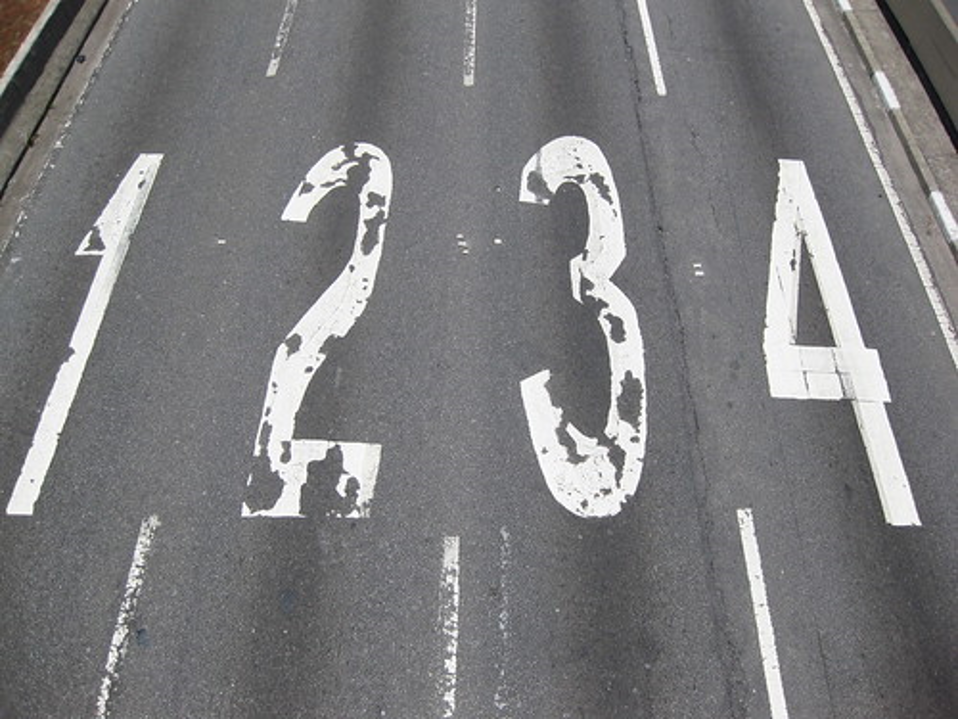
\includegraphics[width=6cm,height=3cm]{C5BM - BM - Q6.png}}},
optionA={Hundreds},
optionB={Tens},
optionC={Thousandths},
optionD={Ones},
correctoption={B},
leftmini={0.5},
rightmini={0.4},}

\begin{minipage}{\linewidth}
\hspace{1cm}
\centering
\tiny
\renewcommand{\arraystretch}{1.25}
\begin{tabular}{|M{1.2cm}|M{0.8cm}|M{0.8cm}|M{0.8cm}|M{0.8cm}|M{0.8cm}|}
\hline
Option & A (\ding{55}) & \cellcolor{cellgreen} B (\ding{51}) & C (\ding{55}) & D (\ding{55}) & E \\ 
\hline
6 A & \highno{13\%} & \highgreen{87\%} & \highno{0\%} & \highno{0\%} & \highno{0\%} \\ 
 \hline 
6 B & \highno{5\%} & \highgreen{89\%} & \highno{5\%} & \highno{0\%} & \highno{0\%} \\ \hline
\end{tabular}
\end{minipage}

\end{frame}
% \input{4. PPT/6. My Answer/Math/C6/117_C6M - Q4}


\begin{frame}[shrink=0.1,label=QPC6QC5BM - BM - Q7]{Q5 [Basic Math]}
\vspace{-0.2cm}
\mcqtextbottomOneFour{
questionnumber={5}, 
questionTag={C5BM - BM - Q7}, 
questiontext={How many digits are greater than 5? \quad 2386452662},
optionA={4},
optionB={5},
optionC={10},
optionD={1},
correctoption={A},}

\begin{minipage}{\linewidth}
\hspace{1cm}
\centering
\tiny
\renewcommand{\arraystretch}{1.25}
\begin{tabular}{|M{1.2cm}|M{0.8cm}|M{0.8cm}|M{0.8cm}|M{0.8cm}|M{0.8cm}|}
\hline
Option & \cellcolor{cellgreen} A (\ding{51}) & B (\ding{55}) & C (\ding{55}) & D (\ding{55}) & E \\ 
\hline
6 A & \highgreen{87\%} & \highno{7\%} & \highno{0\%} & \highno{7\%} & \highno{0\%} \\ 
 \hline 
6 B & \highno{68\%} & \highno{32\%} & \highno{0\%} & \highno{0\%} & \highno{0\%} \\ \hline
\end{tabular}
\end{minipage}

\end{frame}
% \input{4. PPT/6. My Answer/Math/C6/117_C6M - Q5}


\begin{frame}[shrink=0.1,label=QPC6QC5BM - BM - Q3]{Q6 [Basic Math]}
\vspace{-0.2cm}
\mcqtextbottomOneFour{
questionnumber={6}, 
questionTag={C5BM - BM - Q3}, 
questiontext={Multiply : 1798 $\times$ 26  },
optionA={46746},
optionB={46744},
optionC={46748},
optionD={46848},
correctoption={C},}

\begin{minipage}{\linewidth}
\hspace{1cm}
\centering
\tiny
\renewcommand{\arraystretch}{1.25}
\begin{tabular}{|M{1.2cm}|M{0.8cm}|M{0.8cm}|M{0.8cm}|M{0.8cm}|M{0.8cm}|}
\hline
Option & A (\ding{55}) & B (\ding{55}) & \cellcolor{cellgreen} C (\ding{51}) & D (\ding{55}) & E \\ 
\hline
6 A & \highno{0\%} & \highno{13\%} & \highgreen{87\%} & \highno{0\%} & \highno{0\%} \\ 
 \hline 
6 B & \highno{21\%} & \highno{16\%} & \highno{53\%} & \highno{5\%} & \highno{5\%} \\ \hline
\end{tabular}
\end{minipage}

\end{frame}
% \input{4. PPT/6. My Answer/Math/C6/117_C6M - Q6}


\begin{frame}[shrink=0.1,label=QPC6QC5BM - BM - Q2]{Q7 [Basic Math]}
\vspace{-0.2cm}
\mcqimgleftFourOne{
questionnumber={7}, 
questionTag={C5BM - BM - Q2}, 
questiontext={Subtract.},
imgtabletikz  = {
\begin{table}[H]
\centering
\begin{tabular}{cccc}
& 5 & 6 & 4  \\
$-$ & 3 & 7 & 5\\
\hline
& & & \\
\hline
\end{tabular}
\end{table} },
optionA={939},
optionB={211},
optionC={192},
optionD={189},
correctoption={D},
leftmini={0.5},
rightmini={0.4},
}


\begin{minipage}{\linewidth}
\hspace{1cm}
\centering
\tiny
\renewcommand{\arraystretch}{1.25}
\begin{tabular}{|M{1.2cm}|M{0.8cm}|M{0.8cm}|M{0.8cm}|M{0.8cm}|M{0.8cm}|}
\hline
Option & A (\ding{55}) & B (\ding{55}) & C (\ding{55}) & \cellcolor{cellgreen} D (\ding{51}) & E \\ 
\hline
6 A & \highno{0\%} & \highno{7\%} & \highno{7\%} & \highgreen{87\%} & \highno{0\%} \\ 
 \hline 
6 B & \highno{0\%} & \highno{5\%} & \highno{0\%} & \highgreen{95\%} & \highno{0\%} \\ \hline
\end{tabular}
\end{minipage}

\end{frame}
% \input{4. PPT/6. My Answer/Math/C6/117_C6M - Q7}


\begin{frame}[shrink=0.1,label=QPC6QC6M01 - DT - Q6]{Q20 [1. Knowing Our Numbers]}
\vspace{-0.2cm}
\mcqimgleftFourOne{
questionnumber={20}, 
questiontext={Add. },
imgtabletikz  = {  
\renewcommand{\arraystretch}{1.5}
\begin{tabular}{cccccc}
  & 8 & 2 & 5 & 7 & 0  \\
 + & 5 & 8 & 3 & 2 & 0 \\
 \hline
 &&&&&\\
 \hline
\end{tabular} },
optionA={1310890},
optionB={140980},
optionC={140890},
optionD={14890},
questionTag={C6M01 - DT - Q6},
leftmini={0.5},
rightmini={0.4},
correctoption={C},
}

\begin{minipage}{\linewidth}
\hspace{1cm}
\centering
\tiny
\renewcommand{\arraystretch}{1.25}
\begin{tabular}{|M{1.2cm}|M{0.8cm}|M{0.8cm}|M{0.8cm}|M{0.8cm}|M{0.8cm}|}
\hline
Option & A (\ding{55}) & B (\ding{55}) & \cellcolor{cellgreen} C (\ding{51}) & D (\ding{55}) & E \\ 
\hline
6 A & \highno{0\%} & \highno{0\%} & \highgreen{100\%} & \highno{0\%} & \highno{0\%} \\ 
 \hline 
6 B & \highno{11\%} & \highno{0\%} & \highgreen{89\%} & \highno{0\%} & \highno{0\%} \\ \hline
\end{tabular}
\end{minipage}

\end{frame}
% \input{4. PPT/6. My Answer/Math/C6/117_C6M - Q20}


\begin{frame}[shrink=0.1,label=QPC6QC6M01 - DT - Q5]{Q22 [1. Knowing Our Numbers]}
\vspace{-0.2cm}
\mcqimgleftFourOne{
questionnumber={22}, 
questiontext={Compare.},
imgtabletikz = { 
\tikzset{every picture/.style={line width=0.75pt,scale=\scalefactor}} 
\begin{tikzpicture}[x=0.75pt,y=0.75pt,yscale=-1,xscale=1]
\draw (158.5,90.5) node  {\adjustbox{scale=\scalefactor}{
\includegraphics[width=74.25pt,height=55pt]{C6M01 - DT - Q5i.png}}};
\draw (354.5,89.5) node  {\adjustbox{scale=\scalefactor}{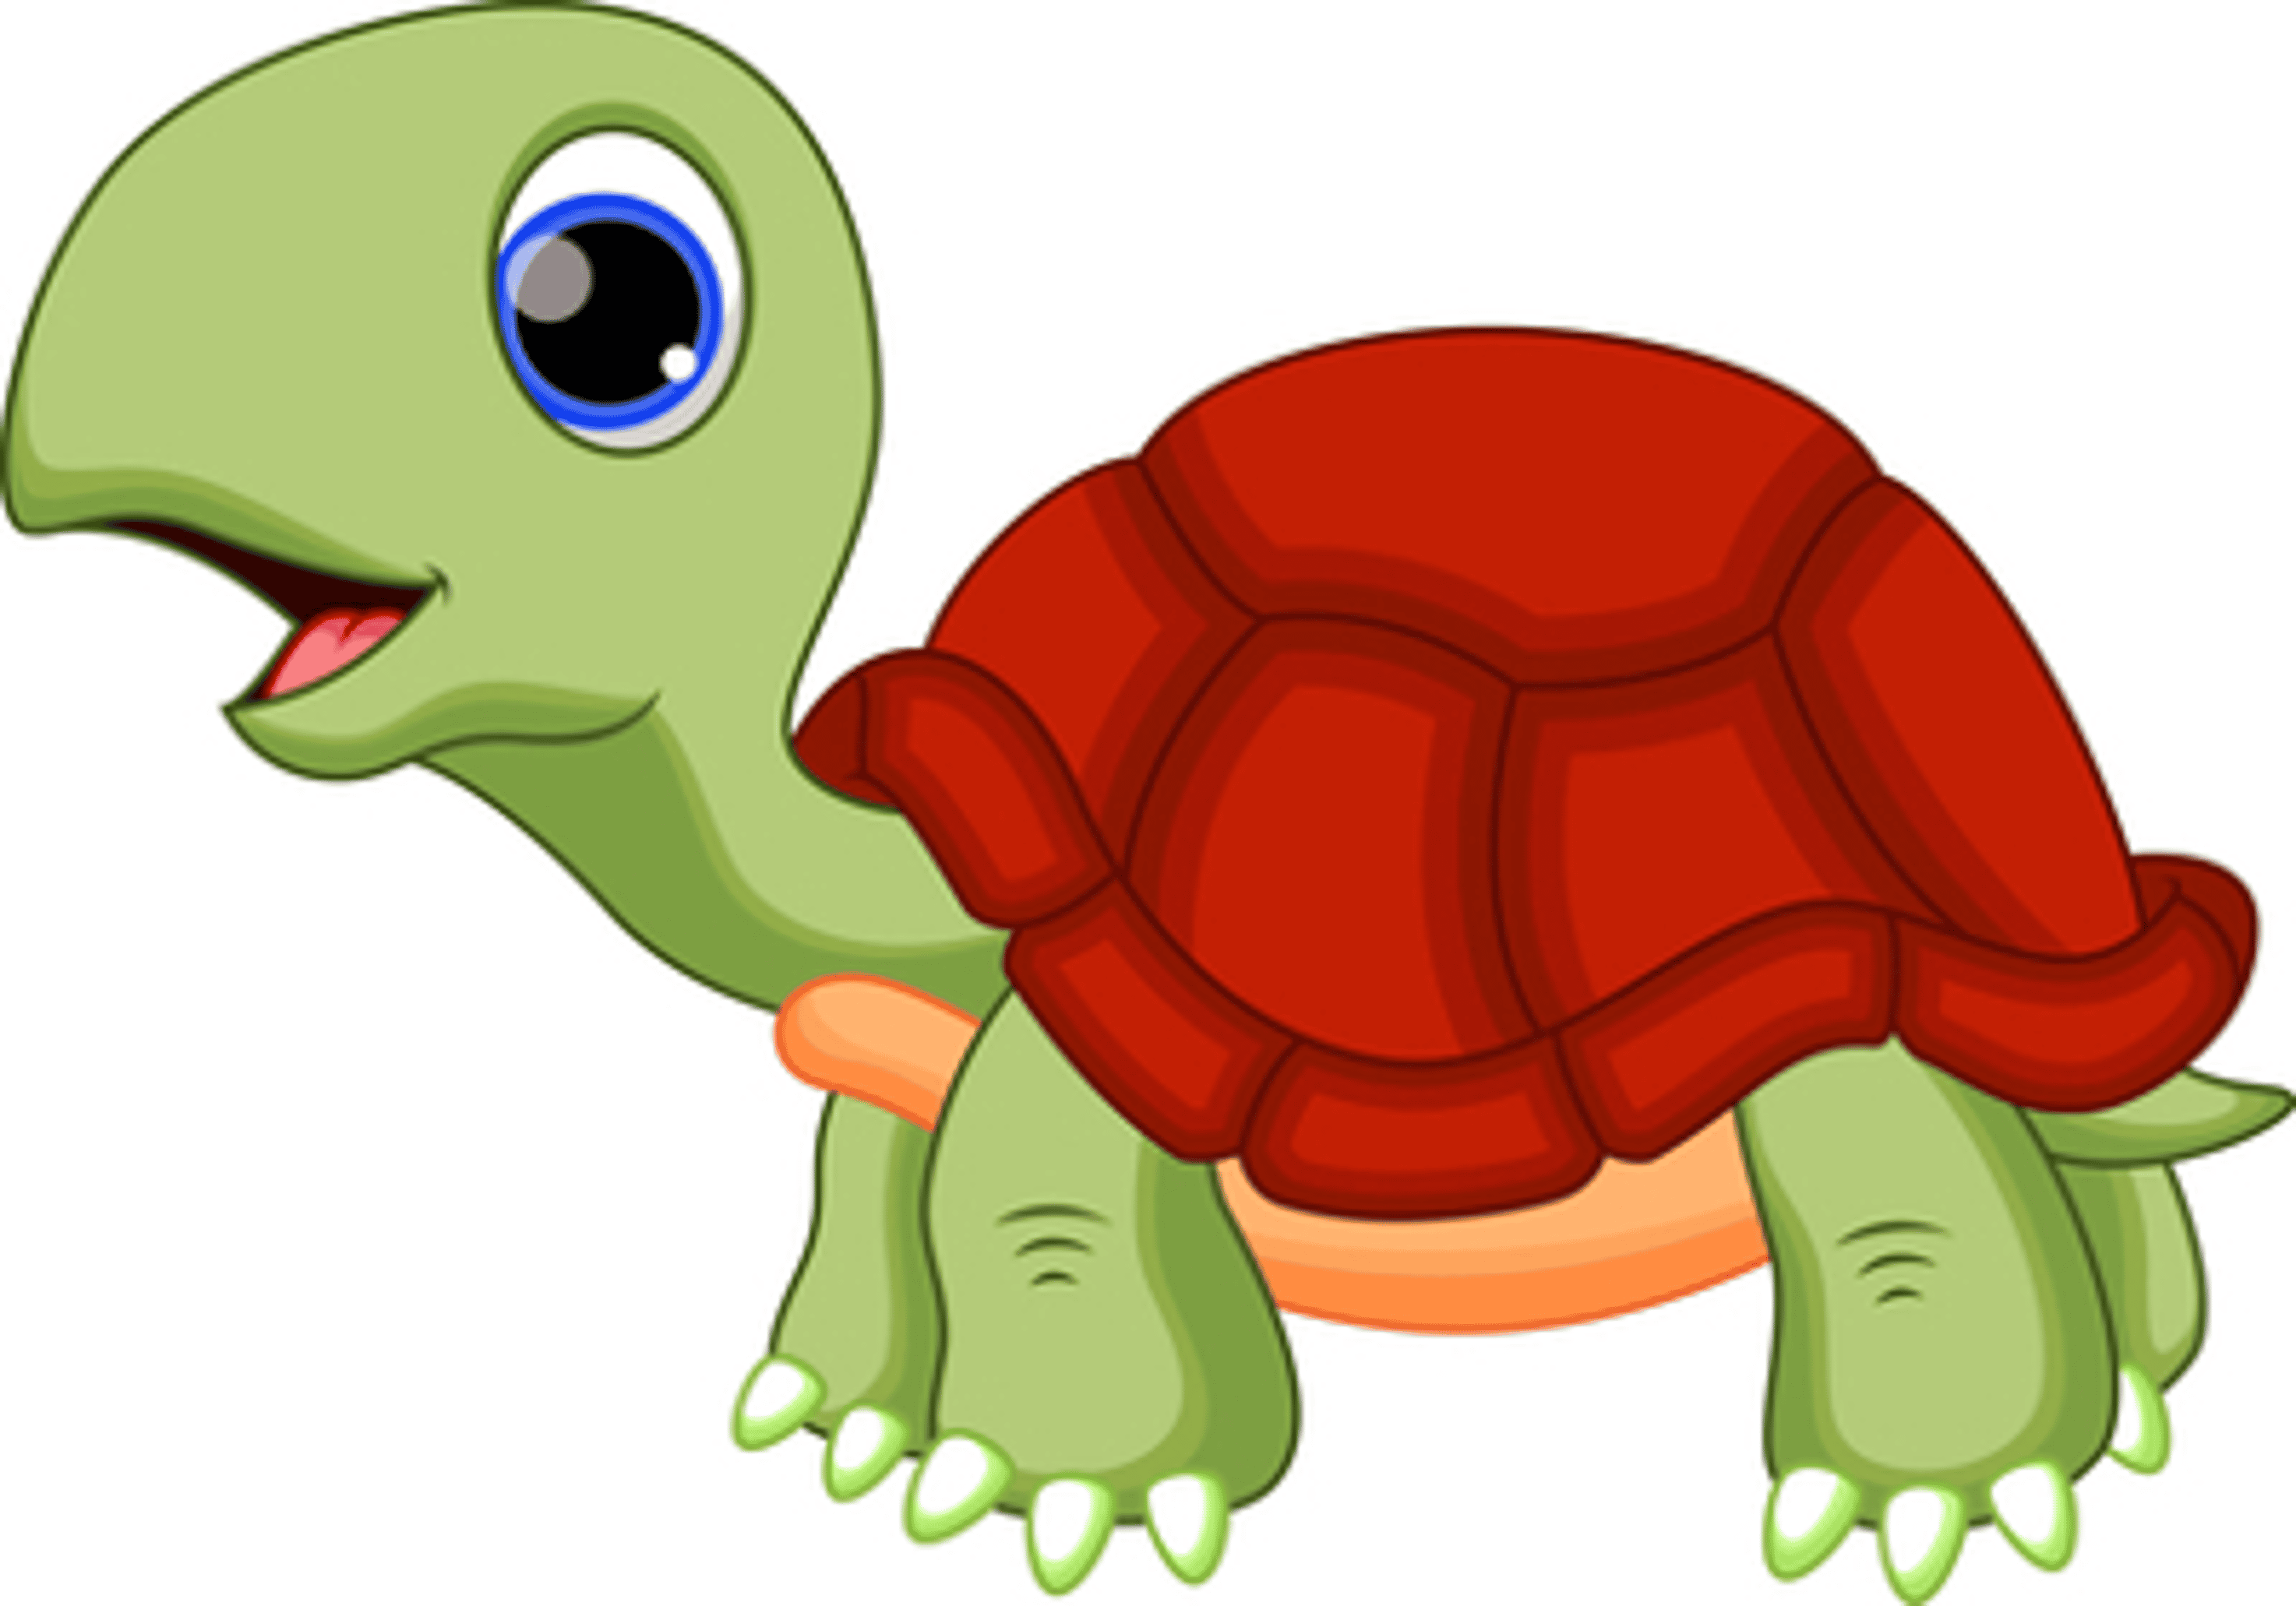
\includegraphics[width=74.25pt,height=55pt]{C6M01 - DT - Q5ii.png}}};
\draw   (243,76) -- (276,76) -- (276,109) -- (243,109) -- cycle ;
\draw (88,133) node [anchor=north west][inner sep=0.75pt]   [align=left] {150000 green tortoise};
\draw (294,133) node [anchor=north west][inner sep=0.75pt]   [align=left] {130000 red tortoise};
\end{tikzpicture} },
optionA={$<$},
optionB={$>$},
optionC={$=$},
optionD={None of the above},
questionTag={C6M01 - DT - Q5}, 
leftmini={0.5},
rightmini={0.4},
correctoption={B},
}

\begin{minipage}{\linewidth}
\hspace{1cm}
\centering
\tiny
\renewcommand{\arraystretch}{1.25}
\begin{tabular}{|M{1.2cm}|M{0.8cm}|M{0.8cm}|M{0.8cm}|M{0.8cm}|M{0.8cm}|}
\hline
Option & A (\ding{55}) & \cellcolor{cellgreen} B (\ding{51}) & C (\ding{55}) & D (\ding{55}) & E \\ 
\hline
6 A & \highno{0\%} & \highgreen{93\%} & \highno{7\%} & \highno{0\%} & \highno{0\%} \\ 
 \hline 
6 B & \highno{5\%} & \highgreen{95\%} & \highno{0\%} & \highno{0\%} & \highno{0\%} \\ \hline
\end{tabular}
\end{minipage}

\end{frame}
% \input{4. PPT/6. My Answer/Math/C6/117_C6M - Q22}


\begin{frame}[shrink=0.1,label=QPC6QC6M01 - DT - Q3]{Q24 [1. Knowing Our Numbers]}
\vspace{-0.2cm}
\mcqtextbottomOneFour{
questionnumber={24}, 
questiontext={In 231056, find the number that represents lakhs.},
optionA={2},
optionB={5},
optionC={3},
optionD={0},
questionTag={C6M01 - DT - Q3}, 
correctoption={A},
}

\begin{minipage}{\linewidth}
\hspace{1cm}
\centering
\tiny
\renewcommand{\arraystretch}{1.25}
\begin{tabular}{|M{1.2cm}|M{0.8cm}|M{0.8cm}|M{0.8cm}|M{0.8cm}|M{0.8cm}|}
\hline
Option & \cellcolor{cellgreen} A (\ding{51}) & B (\ding{55}) & C (\ding{55}) & D (\ding{55}) & E \\ 
\hline
6 A & \highgreen{93\%} & \highno{7\%} & \highno{0\%} & \highno{0\%} & \highno{0\%} \\ 
 \hline 
6 B & \highgreen{79\%} & \highno{5\%} & \highno{11\%} & \highno{5\%} & \highno{0\%} \\ \hline
\end{tabular}
\end{minipage}

\end{frame}
% \input{4. PPT/6. My Answer/Math/C6/117_C6M - Q24}


\begin{frame}[shrink=0.1,label=QPC6QC6M03 - DT - Q6]{Q50 [2. Whole Numbers]}
\vspace{-0.2cm}
\mcqtextbottomOneFour{
questionnumber={50}, 
questiontext={Find the predecessor of Tuesday.},
optionA={Tuesday},
optionB={Wednesday },
optionC={Monday },
optionD={Sunday},
questionTag={C6M03 - DT - Q6}, 
correctoption={C},
}

\begin{minipage}{\linewidth}
\hspace{1cm}
\centering
\tiny
\renewcommand{\arraystretch}{1.25}
\begin{tabular}{|M{1.2cm}|M{0.8cm}|M{0.8cm}|M{0.8cm}|M{0.8cm}|M{0.8cm}|}
\hline
Option & A (\ding{55}) & B (\ding{55}) & \cellcolor{cellgreen} C (\ding{51}) & D (\ding{55}) & E \\ 
\hline
6 A & \highno{7\%} & \highno{27\%} & \highno{67\%} & \highno{0\%} & \highno{0\%} \\ 
 \hline 
6 B & \highno{0\%} & \highno{16\%} & \highgreen{79\%} & \highno{5\%} & \highno{0\%} \\ \hline
\end{tabular}
\end{minipage}

\end{frame}
% \input{4. PPT/6. My Answer/Math/C6/117_C6M - Q50}


\begin{frame}[shrink=0.1,label=QPC6QC6M03 - CT - Q1]{Q59 [2. Whole Numbers]}
\vspace{-0.2cm}
\mcqimgleftFourOne{
questionnumber={59 - Critical Thinking},
questionTag = {C6M03 - CT - Q1},
questiontext = {Find the value of $y$ by solving the cross puzzle.},
imgtabletikz = { 
\begin{table}[H]
\centering
\renewcommand{\arraystretch}{1.25}
\begin{tabular}{ccccccccc}
   \cline{1-5}
   \multicolumn{1}{|c|}{10}& \multicolumn{1}{|c|}{+} & \multicolumn{1}{|c|}{25} & \multicolumn{1}{|c|}{=} & \multicolumn{1}{|c|}{35} &&&&\\
   \cline{1-5}
   &&&&\multicolumn{1}{|c|}{$-$} &&&&\\
   \cline{5-5}
   &&&& \multicolumn{1}{|c|}{$x$} &&&&\\
   \cline{5-5}
   &&&& \multicolumn{1}{|c|}{=} &&&&\\
   \cline{5-9}
   &&&&\multicolumn{1}{|c|}{35} &\multicolumn{1}{|c|}{$\times$} & \multicolumn{1}{|c|}{$x$}& \multicolumn{1}{|c|}{=} & \multicolumn{1}{|c|}{$y$}\\
   \cline{5-9}
\end{tabular}
\end{table}  },
optionA={0},
optionB={1},
optionC={35},
optionD={70},
correctoption = {A},
leftmini={0.6},
rightmini={0.3},
}

\begin{minipage}{\linewidth}
\hspace{1cm}
\centering
\tiny
\renewcommand{\arraystretch}{1.25}
\begin{tabular}{|M{1.2cm}|M{0.8cm}|M{0.8cm}|M{0.8cm}|M{0.8cm}|M{0.8cm}|}
\hline
Option & \cellcolor{cellgreen} A (\ding{51}) & B (\ding{55}) & C (\ding{55}) & D (\ding{55}) & E \\ 
\hline
6 A & \highred{20\%} & \highno{0\%} & \highno{53\%} & \highno{20\%} & \highno{7\%} \\ 
 \hline 
6 B & \highred{21\%} & \highno{26\%} & \highno{26\%} & \highno{21\%} & \highno{5\%} \\ \hline
\end{tabular}
\end{minipage}

\end{frame}
% \input{4. PPT/6. My Answer/Math/C6/117_C6M - Q59 - Critical Thinking}


\begin{frame}[shrink=0.1,label=QPC6QC6M04 - DT - Q8]{Q12 [3. Playing with Numbers]}
\vspace{-0.2cm}
\mcqimgleftFourOne{
questionnumber={12}, 
questiontext={Find the number in the circle by completing the given LCM. },
imgtabletikz  = { 
\renewcommand{\arraystretch}{1.25}
\begin{tabular}{p{1cm}|p{0.5cm}p{1cm}}
  \RaggedLeft{2} & 4, & 6 \\
  \cline{2-3}
  \RaggedLeft{2} & 2,& \rule{20pt}{0.5pt}\\
  \cline{2-3}
  \RaggedLeft{{\large{\textcircled{\rule{10pt}{0.5pt}}}}} & \rule{20pt}{0.5pt}, & 3 \\
  \cline{2-3}
  & 1,& 1 \\
  \cline{2-3}          
\end{tabular}
},
optionA={1},
optionB={2},
optionC={0},
optionD={3},
questionTag={C6M04 - DT - Q8}, 
leftmini={0.5},
rightmini={0.4},
correctoption={D},
}

\begin{minipage}{\linewidth}
\hspace{1cm}
\centering
\tiny
\renewcommand{\arraystretch}{1.25}
\begin{tabular}{|M{1.2cm}|M{0.8cm}|M{0.8cm}|M{0.8cm}|M{0.8cm}|M{0.8cm}|}
\hline
Option & A (\ding{55}) & B (\ding{55}) & C (\ding{55}) & \cellcolor{cellgreen} D (\ding{51}) & E \\ 
\hline
6 A & \highno{0\%} & \highno{13\%} & \highno{0\%} & \highgreen{87\%} & \highno{0\%} \\ 
 \hline 
6 B & \highno{0\%} & \highno{16\%} & \highno{11\%} & \highno{68\%} & \highno{5\%} \\ \hline
\end{tabular}
\end{minipage}

\end{frame}
% \input{4. PPT/6. My Answer/Math/C6/117_C6M - Q12}


\begin{frame}[shrink=0.1,label=QPC6QC6M04 - DT - Q1]{Q27 [3. Playing with Numbers]}
\vspace{-0.2cm}
\mcqimgleftFourOne{
questionnumber={27}, 
questiontext={Find the image with an odd number count.},
imgtabletikz  = {

\tikzset{every picture/.style={line width=0.75pt,scale=\scalefactor}} 
\begin{tikzpicture}[x=0.75pt,y=0.75pt,yscale=-1,xscale=1]
\draw (178.5,110.5) node  {\adjustbox{scale=\scalefactor}{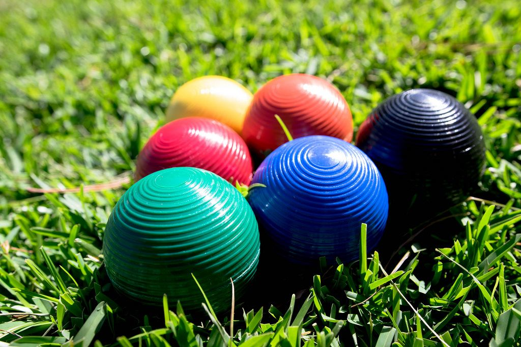
\includegraphics[width=80pt,height=60pt]{C6M04 - DT - Q1i.png}}};
\draw (374.5,109.5) node  {\adjustbox{scale=\scalefactor}{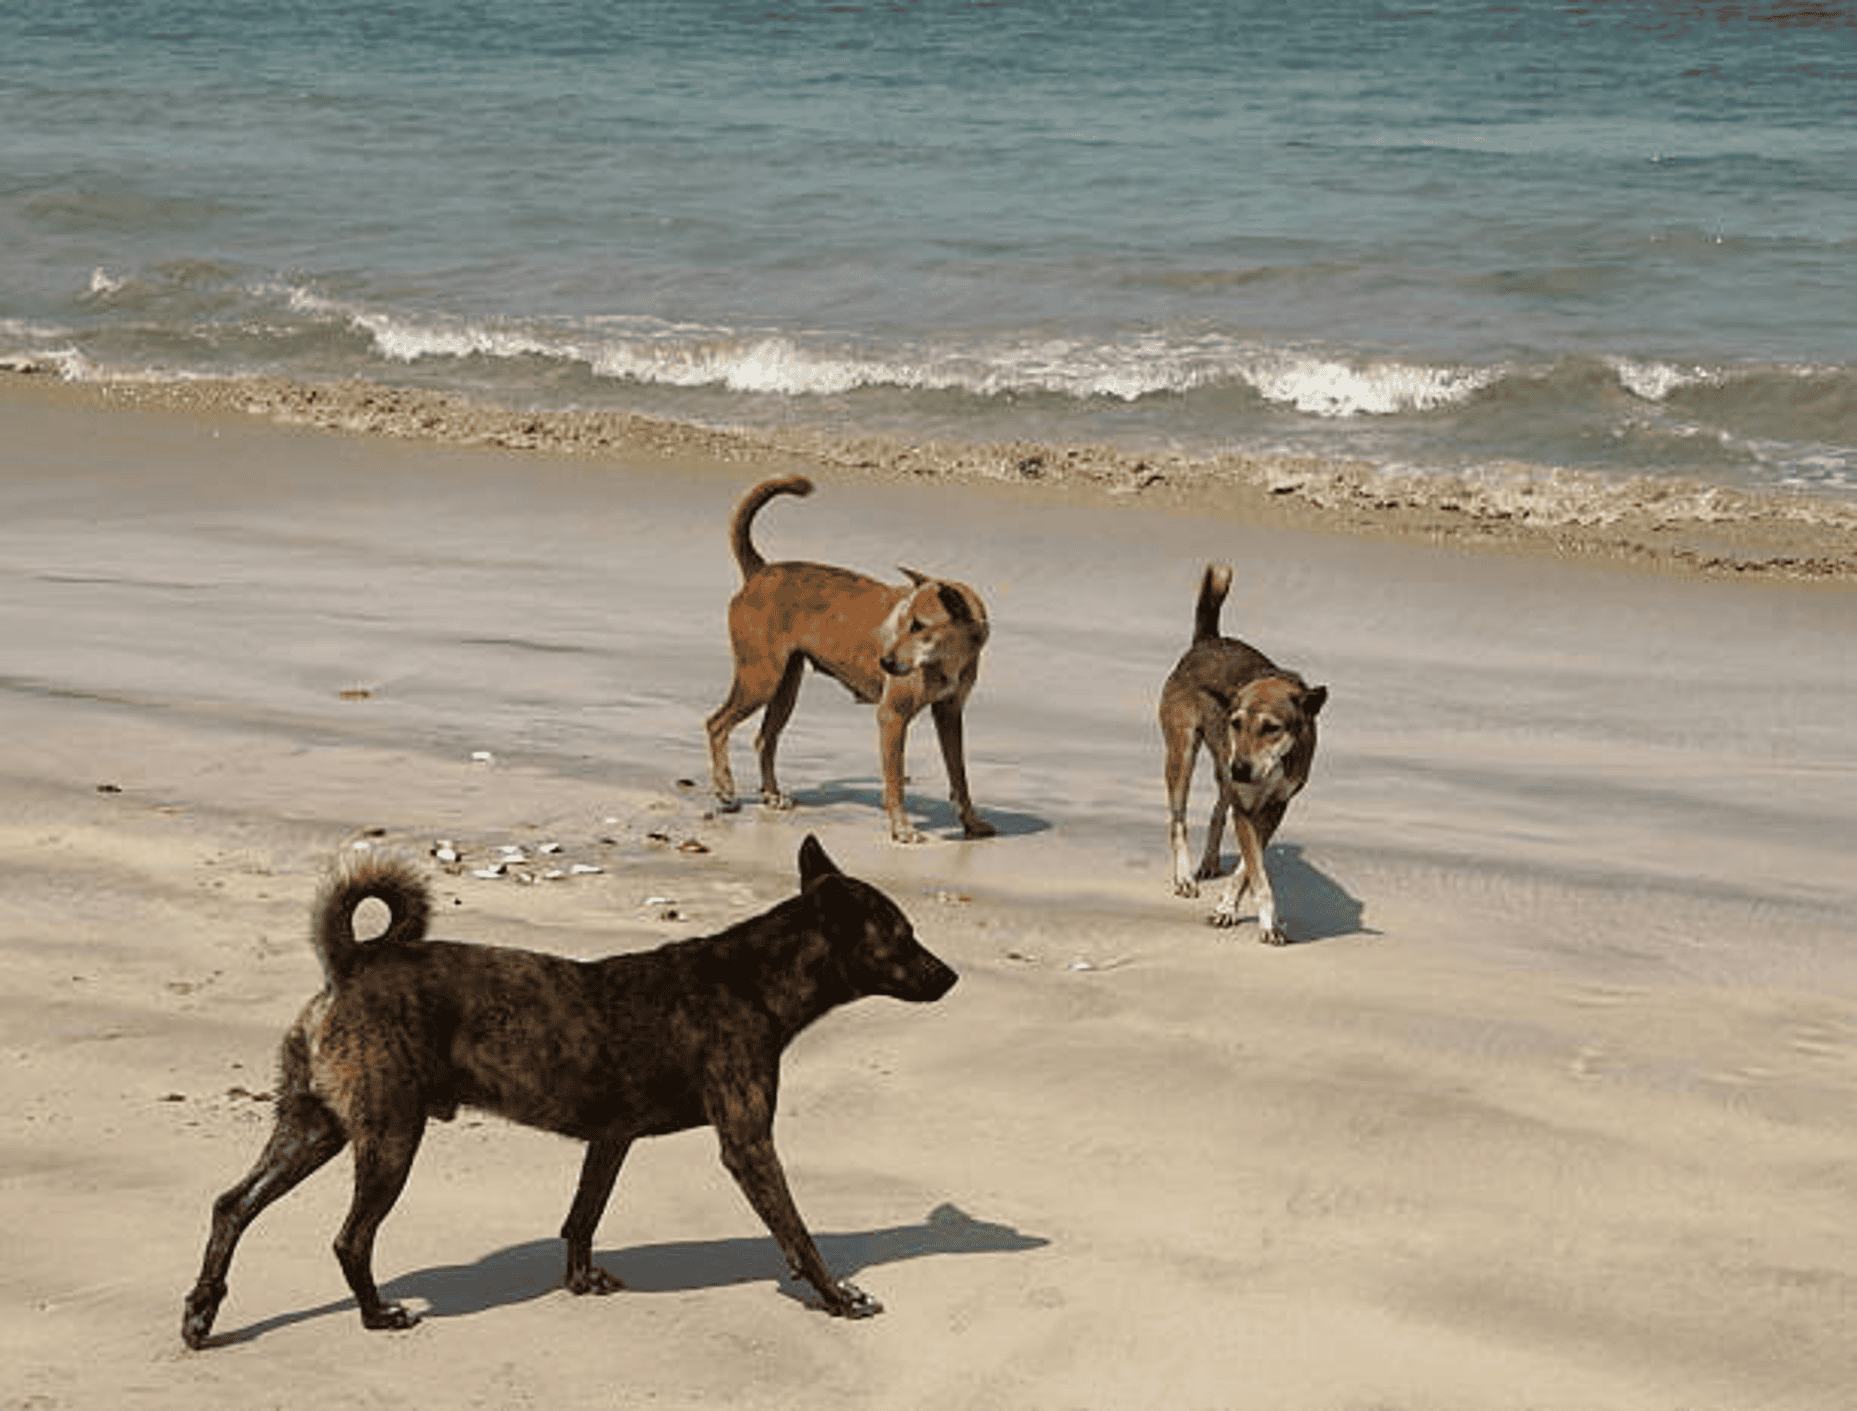
\includegraphics[width=80pt,height=60pt]{C6M04 - DT - Q1ii.png}}};
\draw (90,155) node [anchor=north west][inner sep=0.75pt]   [align=left] {Number of balls = \rule{40pt}{0.5pt}};
\draw (295,155) node [anchor=north west][inner sep=0.75pt]   [align=left] {Number of dogs = \rule{40pt}{0.5pt}};
\end{tikzpicture}  
},
optionA={Balls},
optionB={Dogs},
optionC={Both balls and dogs},
optionD={None of these},
questionTag={C6M04 - DT - Q1}, 
leftmini={0.5},
rightmini={0.35},
correctoption={B},
}

\begin{minipage}{\linewidth}
\hspace{1cm}
\centering
\tiny
\renewcommand{\arraystretch}{1.25}
\begin{tabular}{|M{1.2cm}|M{0.8cm}|M{0.8cm}|M{0.8cm}|M{0.8cm}|M{0.8cm}|}
\hline
Option & A (\ding{55}) & \cellcolor{cellgreen} B (\ding{51}) & C (\ding{55}) & D (\ding{55}) & E \\ 
\hline
6 A & \highno{13\%} & \highno{73\%} & \highno{13\%} & \highno{0\%} & \highno{0\%} \\ 
 \hline 
6 B & \highno{5\%} & \highno{74\%} & \highno{11\%} & \highno{11\%} & \highno{0\%} \\ \hline
\end{tabular}
\end{minipage}

\end{frame}
% \input{4. PPT/6. My Answer/Math/C6/117_C6M - Q27}


\begin{frame}[shrink=0.1,label=QPC6QC6M04 - DT - Q6]{Q29 [3. Playing with Numbers]}
\vspace{-0.2cm}
\mcqimgleftFourOne{
questionnumber={29}, 
questiontext={The given amount is divisible by \rule{40pt}{0.5pt}.},
imgtabletikz = { 
\adjustbox{scale=\scalefactor}{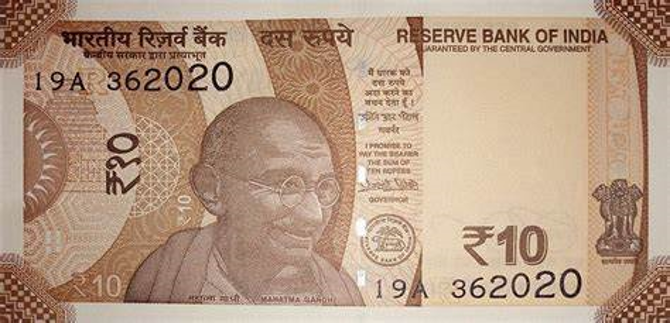
\includegraphics[width=6cm, height=2.5cm]{C6M04 - DT - Q6.png}} },
optionA={5},
optionB={3},
optionC={4},
optionD={6},
questionTag={C6M04 - DT - Q6}, 
leftmini={0.4},
rightmini={0.4},
correctoption={A},
}

\begin{minipage}{\linewidth}
\hspace{1cm}
\centering
\tiny
\renewcommand{\arraystretch}{1.25}
\begin{tabular}{|M{1.2cm}|M{0.8cm}|M{0.8cm}|M{0.8cm}|M{0.8cm}|M{0.8cm}|}
\hline
Option & \cellcolor{cellgreen} A (\ding{51}) & B (\ding{55}) & C (\ding{55}) & D (\ding{55}) & E \\ 
\hline
6 A & \highgreen{100\%} & \highno{0\%} & \highno{0\%} & \highno{0\%} & \highno{0\%} \\ 
 \hline 
6 B & \highgreen{95\%} & \highno{5\%} & \highno{0\%} & \highno{0\%} & \highno{0\%} \\ \hline
\end{tabular}
\end{minipage}

\end{frame}
% \input{4. PPT/6. My Answer/Math/C6/117_C6M - Q29}


\begin{frame}[shrink=0.1,label=QPC6QC6M04 - DT - Q7]{Q37 [3. Playing with Numbers]}
\vspace{-0.2cm}
\mcqtextbottomOneFour{
questionnumber={37}, 
questiontext={Find the prime factorisation of 18.},
optionA={ 2 $\times$ 6 $\times$ 1},
optionB={6 $\times$ 1 $\times$ 3},
optionC={2 $\times$ 3 $\times$ 3},
optionD={2 $\times$ 2 $\times$ 3},
questionTag={C6M04 - DT - Q7},
correctoption={C},
}

\begin{minipage}{\linewidth}
\hspace{1cm}
\centering
\tiny
\renewcommand{\arraystretch}{1.25}
\begin{tabular}{|M{1.2cm}|M{0.8cm}|M{0.8cm}|M{0.8cm}|M{0.8cm}|M{0.8cm}|}
\hline
Option & A (\ding{55}) & B (\ding{55}) & \cellcolor{cellgreen} C (\ding{51}) & D (\ding{55}) & E \\ 
\hline
6 A & \highno{0\%} & \highno{20\%} & \highgreen{80\%} & \highno{0\%} & \highno{0\%} \\ 
 \hline 
6 B & \highno{5\%} & \highno{32\%} & \highno{53\%} & \highno{5\%} & \highno{5\%} \\ \hline
\end{tabular}
\end{minipage}

\end{frame}
\begin{frame}{Q37 - My Answer Responses}
    \vspace{-0.6cm}
    \begin{multicols}{4}

    % Image: Q37_D117135_Math.png - Scaled height: 6.81mm
    \begin{minipage}{\linewidth}
    \RaggedRight\textbf{\tiny \highgreen{Dheeresh J A [C]}} \\ 
    \vspace{4.00pt}\fcolorbox{blue}{white}{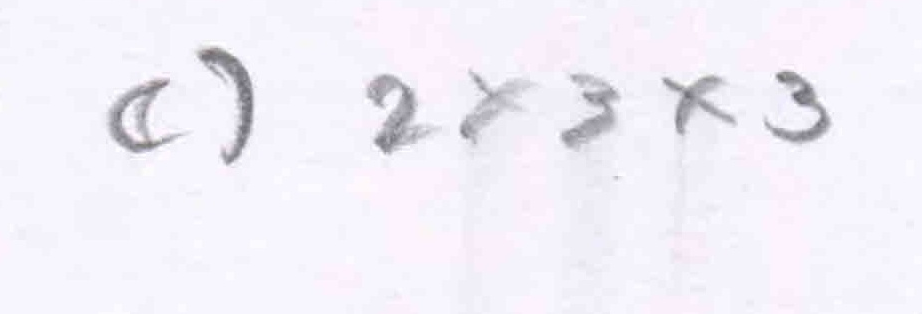
\includegraphics[width=2cm]{Q37_D117135_Math.png}}
    \end{minipage}
    \vspace{10pt}

    % Image: Q37_D117140_Math.png - Scaled height: 12.48mm
    \begin{minipage}{\linewidth}
    \RaggedRight\textbf{\tiny \highgreen{Sabarish B [C]}} \\ 
    \vspace{4.00pt}\fcolorbox{blue}{white}{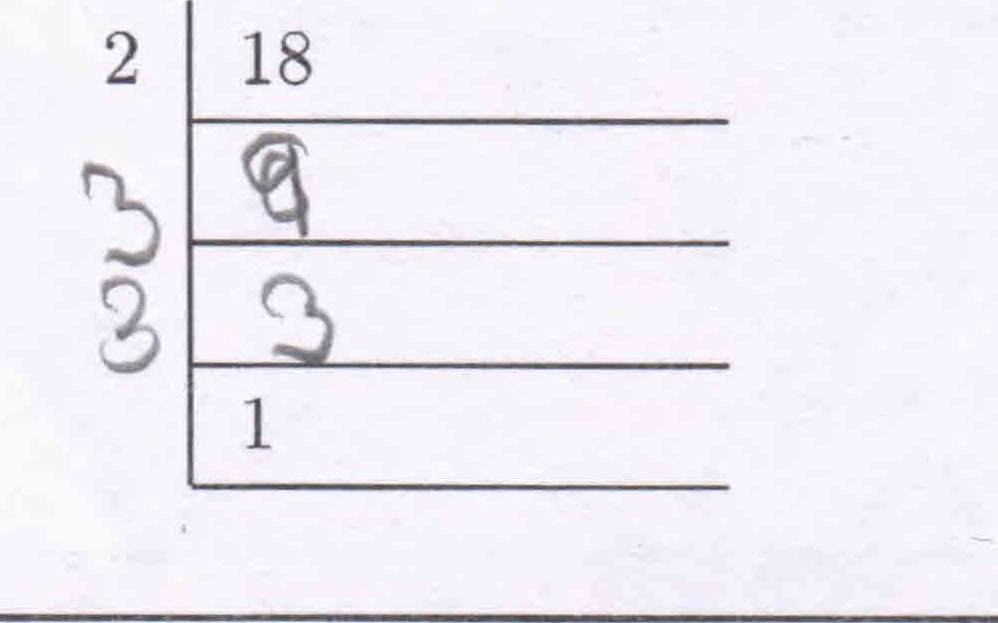
\includegraphics[width=2cm]{Q37_D117140_Math.png}}
    \end{minipage}
    \vspace{10pt}

    % Image: Q37_D117144_Math.png - Scaled height: 13.33mm
    \begin{minipage}{\linewidth}
    \RaggedRight\textbf{\tiny \highgreen{Varshanth K [C]}} \\ 
    \vspace{4.00pt}\fcolorbox{blue}{white}{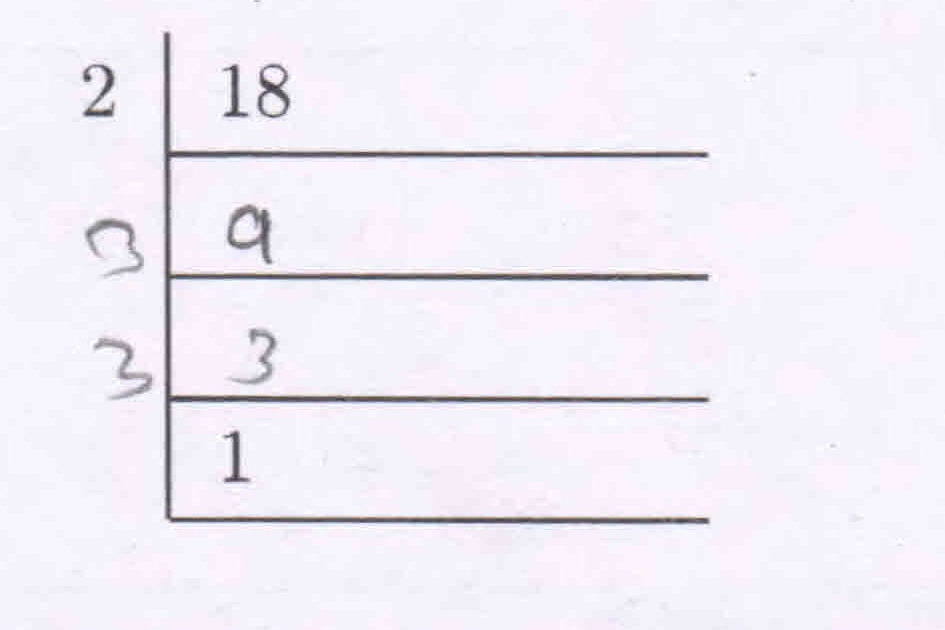
\includegraphics[width=2cm]{Q37_D117144_Math.png}}
    \end{minipage}
    \vspace{10pt}

    % Image: Q37_D117151_Math.png - Scaled height: 6.52mm
    \begin{minipage}{\linewidth}
    \RaggedRight\textbf{\tiny \highgreen{Karnika R [C]}} \\ 
    \vspace{4.00pt}\fcolorbox{blue}{white}{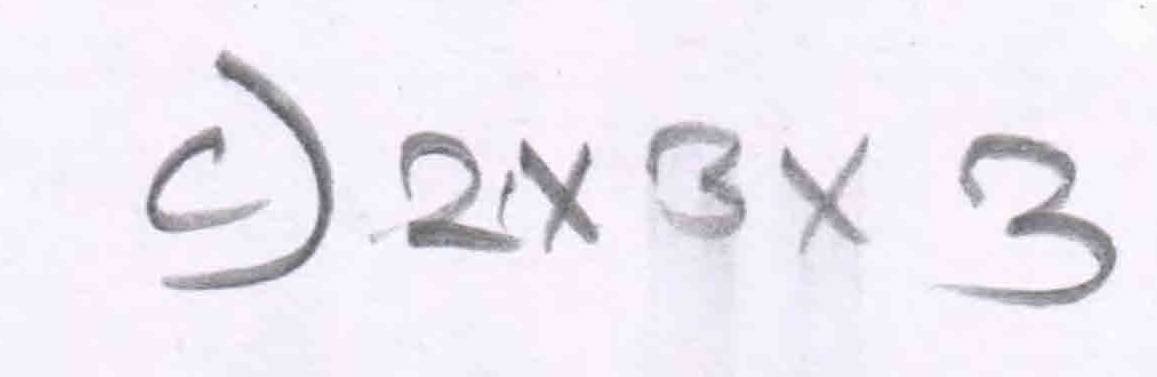
\includegraphics[width=2cm]{Q37_D117151_Math.png}}
    \end{minipage}
    \vspace{10pt}

    % Image: Q37_D117152_Math.png - Scaled height: 13.58mm
    \begin{minipage}{\linewidth}
    \RaggedRight\textbf{\tiny \highgreen{Preethi T [C]}} \\ 
    \vspace{4.00pt}\fcolorbox{blue}{white}{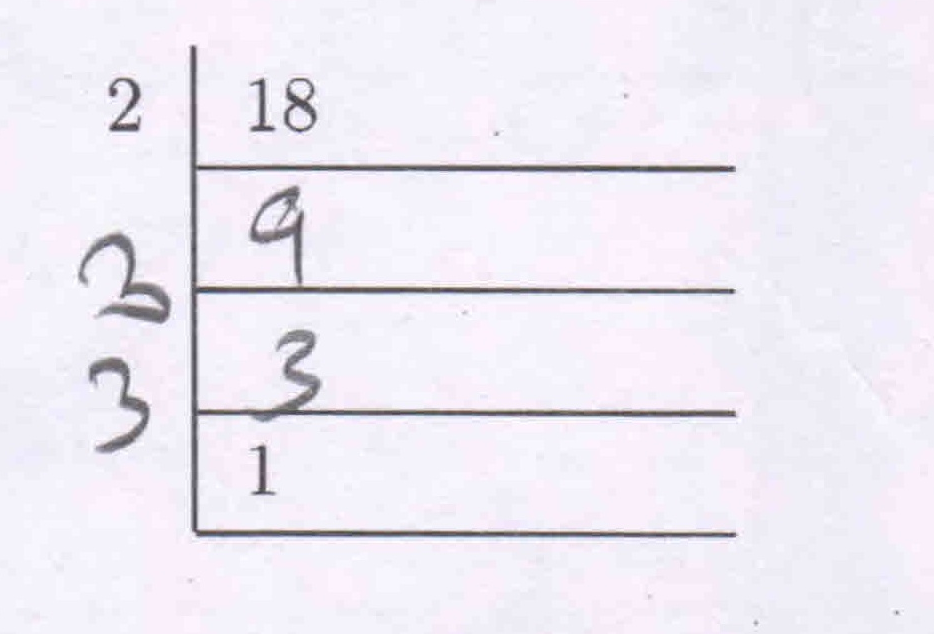
\includegraphics[width=2cm]{Q37_D117152_Math.png}}
    \end{minipage}
    \vspace{10pt}

    % Image: Q37_D117153_Math.png - Scaled height: 7.66mm
    \begin{minipage}{\linewidth}
    \RaggedRight\textbf{\tiny \highred{Priyadharshini S A [B]}} \\ 
    \vspace{4.00pt}\fcolorbox{blue}{white}{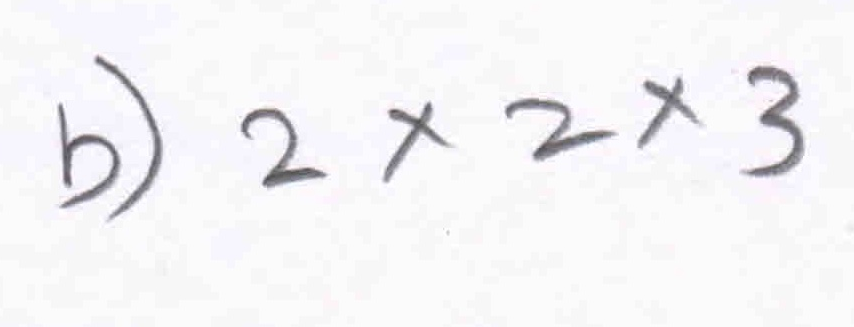
\includegraphics[width=2cm]{Q37_D117153_Math.png}}
    \end{minipage}
    \vspace{10pt}

    % Image: Q37_D117157_Math.png - Scaled height: 4.88mm
    \begin{minipage}{\linewidth}
    \RaggedRight\textbf{\tiny \highred{Aswin P [B]}} \\ 
    \vspace{4.00pt}\fcolorbox{blue}{white}{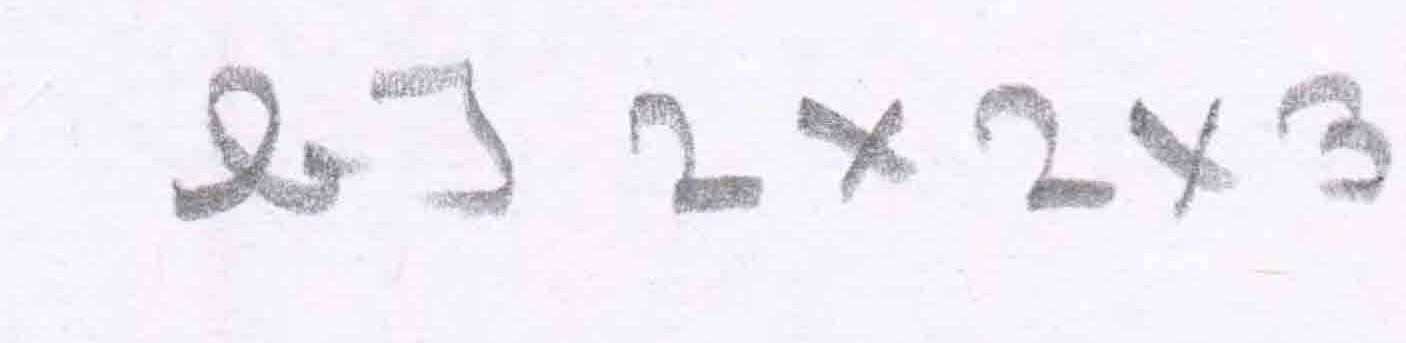
\includegraphics[width=2cm]{Q37_D117157_Math.png}}
    \end{minipage}
    \vspace{10pt}

    % Image: Q37_D117163_Math.png - Scaled height: 7.45mm
    \begin{minipage}{\linewidth}
    \RaggedRight\textbf{\tiny \highgreen{Manjunath A [C]}} \\ 
    \vspace{4.00pt}\fcolorbox{blue}{white}{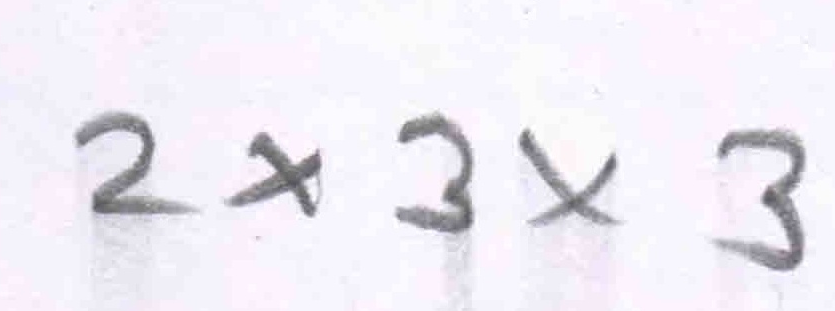
\includegraphics[width=2cm]{Q37_D117163_Math.png}}
    \end{minipage}
    \vspace{10pt}

    % Image: Q37_D117171_Math.png - Scaled height: 4.89mm
    \begin{minipage}{\linewidth}
    \RaggedRight\textbf{\tiny \highgreen{Elakyaa N [C]}} \\ 
    \vspace{4.00pt}\fcolorbox{blue}{white}{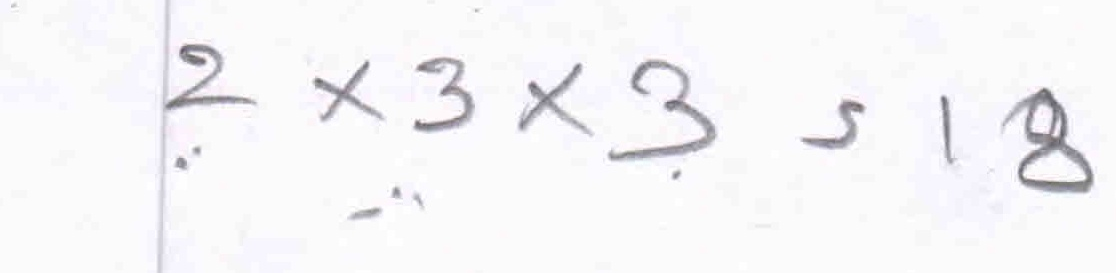
\includegraphics[width=2cm]{Q37_D117171_Math.png}}
    \end{minipage}
    \vspace{10pt}

    % Image: Q37_D117172_Math.png - Scaled height: 14.64mm
    \begin{minipage}{\linewidth}
    \RaggedRight\textbf{\tiny \highred{Raksha Nivasini K S [B]}} \\ 
    \vspace{4.00pt}\fcolorbox{blue}{white}{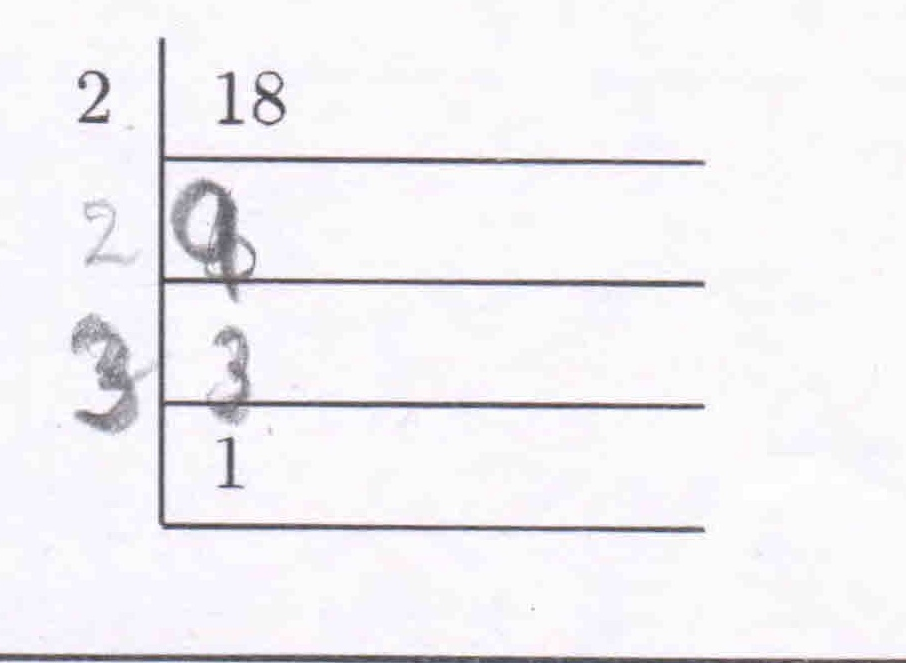
\includegraphics[width=2cm]{Q37_D117172_Math.png}}
    \end{minipage}
    \vspace{10pt}

    \end{multicols}
\end{frame}




\begin{frame}[shrink=0.1,label=QPC6QC6M04 - DT - Q2]{Q42 [3. Playing with Numbers]}
\vspace{-0.2cm}
\mcqtextbottomOneFour{
questionnumber={42}, 
questiontext={Find all the factors of 8. },
optionA={1, 2, 8},
optionB={1, 2, 4, 8},
optionC={1, 2, 6},
optionD={4, 6, 8},
questionTag={C6M04 - DT - Q2}, 
correctoption={B},
}

\begin{minipage}{\linewidth}
\hspace{1cm}
\centering
\tiny
\renewcommand{\arraystretch}{1.25}
\begin{tabular}{|M{1.2cm}|M{0.8cm}|M{0.8cm}|M{0.8cm}|M{0.8cm}|M{0.8cm}|}
\hline
Option & A (\ding{55}) & \cellcolor{cellgreen} B (\ding{51}) & C (\ding{55}) & D (\ding{55}) & E \\ 
\hline
6 A & \highno{0\%} & \highgreen{100\%} & \highno{0\%} & \highno{0\%} & \highno{0\%} \\ 
 \hline 
6 B & \highno{0\%} & \highgreen{95\%} & \highno{5\%} & \highno{0\%} & \highno{0\%} \\ \hline
\end{tabular}
\end{minipage}

\end{frame}
\begin{frame}{Q42 - My Answer Responses}
    \vspace{-0.6cm}
    \begin{multicols}{3}

    % Image: Q42_D117135_Math.png - Scaled height: 7.68mm
    \begin{minipage}{\linewidth}
    \RaggedRight\textbf{\tiny \highgreen{Dheeresh J A [B]}} \\ 
    \vspace{4.00pt}\fcolorbox{blue}{white}{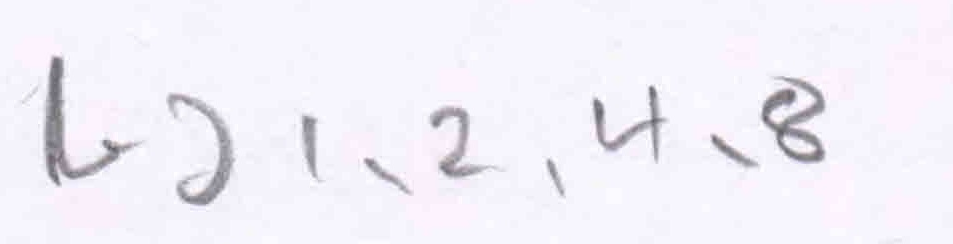
\includegraphics[width=3cm]{Q42_D117135_Math.png}}
    \end{minipage}
    \vspace{10pt}

    % Image: Q42_D117151_Math.png - Scaled height: 8.03mm
    \begin{minipage}{\linewidth}
    \RaggedRight\textbf{\tiny \highgreen{Karnika R [B]}} \\ 
    \vspace{4.00pt}\fcolorbox{blue}{white}{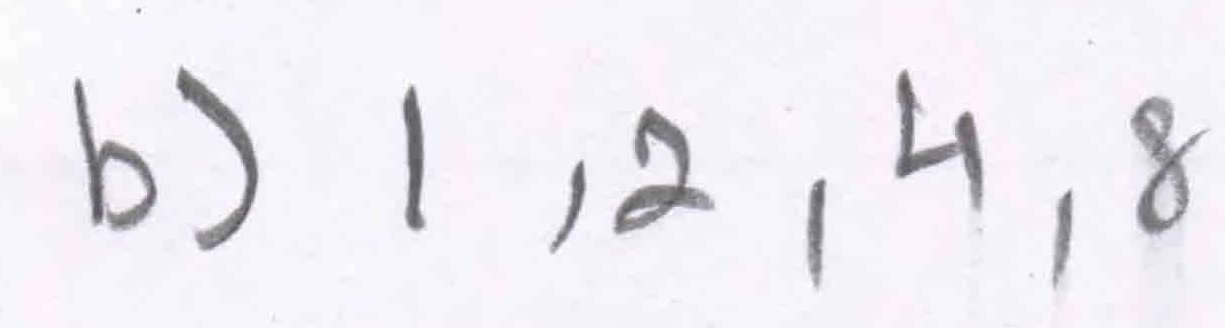
\includegraphics[width=3cm]{Q42_D117151_Math.png}}
    \end{minipage}
    \vspace{10pt}

    % Image: Q42_D117153_Math.png - Scaled height: 8.59mm
    \begin{minipage}{\linewidth}
    \RaggedRight\textbf{\tiny \highgreen{Priyadharshini S A [B]}} \\ 
    \vspace{4.00pt}\fcolorbox{blue}{white}{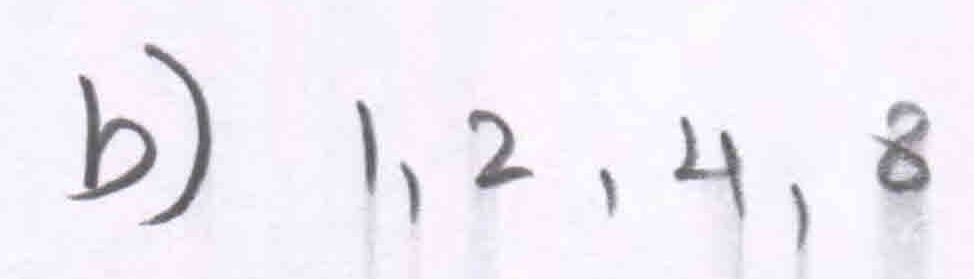
\includegraphics[width=3cm]{Q42_D117153_Math.png}}
    \end{minipage}
    \vspace{10pt}

    % Image: Q42_D117157_Math.png - Scaled height: 7.60mm
    \begin{minipage}{\linewidth}
    \RaggedRight\textbf{\tiny \highgreen{Aswin P [B]}} \\ 
    \vspace{4.00pt}\fcolorbox{blue}{white}{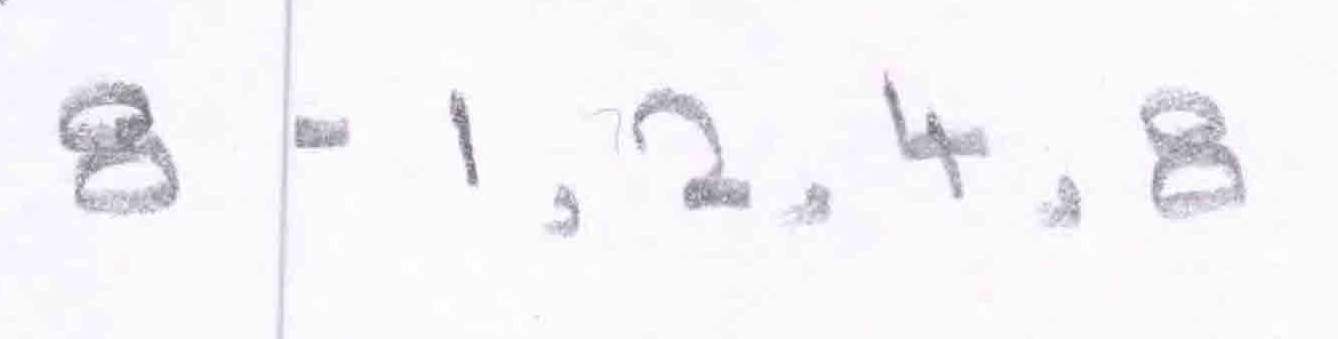
\includegraphics[width=3cm]{Q42_D117157_Math.png}}
    \end{minipage}
    \vspace{10pt}

    % Image: Q42_D117163_Math.png - Scaled height: 7.83mm
    \begin{minipage}{\linewidth}
    \RaggedRight\textbf{\tiny \highgreen{Manjunath A [B]}} \\ 
    \vspace{4.00pt}\fcolorbox{blue}{white}{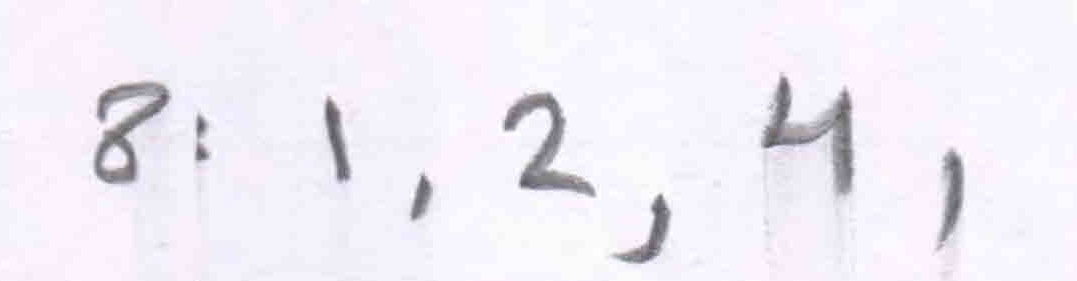
\includegraphics[width=3cm]{Q42_D117163_Math.png}}
    \end{minipage}
    \vspace{10pt}

    % Image: Q42_D117167_Math.png - Scaled height: 6.55mm
    \begin{minipage}{\linewidth}
    \RaggedRight\textbf{\tiny \highgreen{Sriram Karthikeyan V [B]}} \\ 
    \vspace{4.00pt}\fcolorbox{blue}{white}{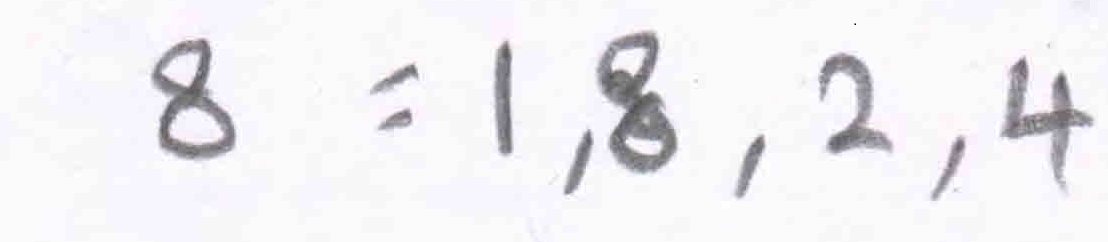
\includegraphics[width=3cm]{Q42_D117167_Math.png}}
    \end{minipage}
    \vspace{10pt}

    % Image: Q42_D117171_Math.png - Scaled height: 5.10mm
    \begin{minipage}{\linewidth}
    \RaggedRight\textbf{\tiny \highgreen{Elakyaa N [B]}} \\ 
    \vspace{4.00pt}\fcolorbox{blue}{white}{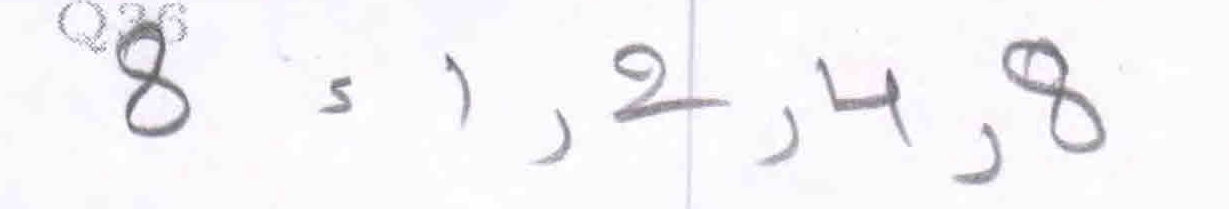
\includegraphics[width=3cm]{Q42_D117171_Math.png}}
    \end{minipage}
    \vspace{10pt}

    \end{multicols}
\end{frame}




\begin{frame}[shrink=0.1,label=QPC6QC6M12 - DT - Q3]{Q9\small [4. Basic Geometrical Ideas \& 5 - Understanding Elementary Shapes]}
\vspace{-0.2cm}

\mcqimgsideFourOne{
questionnumber={9}, 
questiontext={Match the following.},
imgwidth={9cm},
imgheight={4cm},
img={C6M12 - DT - Q3.png},
optionA={i - c, ii - d, iii - a, iv - b},
optionB={i - c, ii - b, iii - a, iv - d},
optionC={i - c, ii - d, iii - b, iv - a},
optionD={i - b, ii - a, iii - c, iv - d},
questionTag={C6M12 – DT – Q3}, 
leftmini={0.4},
rightmini={0.5}, 
correctoption={C},
}

\begin{minipage}{\linewidth}
\hspace{1cm}
\centering
\tiny
\renewcommand{\arraystretch}{1.25}
\begin{tabular}{|M{1.2cm}|M{0.8cm}|M{0.8cm}|M{0.8cm}|M{0.8cm}|M{0.8cm}|}
\hline
Option & A (\ding{55}) & B (\ding{55}) & \cellcolor{cellgreen} C (\ding{51}) & D (\ding{55}) & E \\ 
\hline
6 A & \highno{20\%} & \highno{0\%} & \highgreen{80\%} & \highno{0\%} & \highno{0\%} \\ 
 \hline 
6 B & \highno{16\%} & \highno{21\%} & \highno{58\%} & \highno{0\%} & \highno{5\%} \\ \hline
\end{tabular}
\end{minipage}

\end{frame}
% \input{4. PPT/6. My Answer/Math/C6/117_C6M - Q9}


\begin{frame}[shrink=0.1,label=QPC6QC6M12 - DT - Q1]{Q23\small [4. Basic Geometrical Ideas \& 5 - Understanding Elementary Shapes]}
\vspace{-0.2cm}
\mcqimgleftFourOne{
questionnumber={23}, 
questiontext={Name this polygon.},
imgtabletikz = { 
\tikzset{every picture/.style={line width=0.75pt,scale=\scalefactor}} 
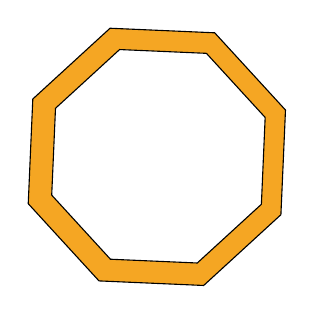
\begin{tikzpicture}[x=0.75pt,y=0.75pt,yscale=-1,xscale=1]
\draw  [fill={rgb, 255:red, 245; green, 166; blue, 35 }  ,fill opacity=1 ] (235.87,155.27) -- (198.66,189.37) -- (148.23,187.17) -- (114.13,149.96) -- (116.33,99.53) -- (153.55,65.43) -- (203.97,67.63) -- (238.08,104.84) -- cycle ;
\draw  [fill={rgb, 255:red, 255; green, 255; blue, 255 }  ,fill opacity=1 ] (226.46,150.25) -- (195.58,178.54) -- (153.74,176.72) -- (125.44,145.84) -- (127.27,104) -- (158.15,75.7) -- (199.99,77.53) -- (228.28,108.41) -- cycle ;
\end{tikzpicture}},
optionA={Square},
optionB={Heptagon},
optionC={Octagon},
optionD={Pentagon},
questionTag={C6M12 - DT - Q1}, 
correctoption={C},
leftmini={0.45},
rightmini={0.45},
}

\begin{minipage}{\linewidth}
\hspace{1cm}
\centering
\tiny
\renewcommand{\arraystretch}{1.25}
\begin{tabular}{|M{1.2cm}|M{0.8cm}|M{0.8cm}|M{0.8cm}|M{0.8cm}|M{0.8cm}|}
\hline
Option & A (\ding{55}) & B (\ding{55}) & \cellcolor{cellgreen} C (\ding{51}) & D (\ding{55}) & E \\ 
\hline
6 A & \highno{0\%} & \highno{0\%} & \highno{67\%} & \highno{33\%} & \highno{0\%} \\ 
 \hline 
6 B & \highno{5\%} & \highno{5\%} & \highno{53\%} & \highno{37\%} & \highno{0\%} \\ \hline
\end{tabular}
\end{minipage}

\end{frame}
% \input{4. PPT/6. My Answer/Math/C6/117_C6M - Q23}


\begin{frame}[shrink=0.1,label=QPC6QC6M12 - DT - Q2]{Q25\small [4. Basic Geometrical Ideas \& 5 - Understanding Elementary Shapes]}
\vspace{-0.2cm}
\mcqtextbottomTwoTwo{
questionnumber={25}, 
questiontext={Find the odd one out. },
optionA={Scalene triangle - three unequal sides},
optionB={Isosceles triangle - two equal sides},
optionC={Equilateral triangle - three equal sides},
optionD={Right angled triangle – all sides equal },
questionTag={C6M12 - DT - Q2}, 
correctoption={D},
}

\begin{minipage}{\linewidth}
\hspace{1cm}
\centering
\tiny
\renewcommand{\arraystretch}{1.25}
\begin{tabular}{|M{1.2cm}|M{0.8cm}|M{0.8cm}|M{0.8cm}|M{0.8cm}|M{0.8cm}|}
\hline
Option & A (\ding{55}) & B (\ding{55}) & C (\ding{55}) & \cellcolor{cellgreen} D (\ding{51}) & E \\ 
\hline
6 A & \highno{20\%} & \highno{0\%} & \highno{7\%} & \highno{73\%} & \highno{0\%} \\ 
 \hline 
6 B & \highno{5\%} & \highno{11\%} & \highno{16\%} & \highno{68\%} & \highno{0\%} \\ \hline
\end{tabular}
\end{minipage}

\end{frame}
% \input{4. PPT/6. My Answer/Math/C6/117_C6M - Q25}


\begin{frame}[shrink=0.1,label=QPC6QC6M11 - DT - Q7]{Q35\small [4. Basic Geometrical Ideas \& 5 - Understanding Elementary Shapes]}
\vspace{-0.2cm}
\mcqtextbottomOneFour{
questionnumber={35}, 
questiontext={Find the figure with an open curve.},
optionA={
\tikzset{every picture/.style={line width=0.75pt,scale=\scalefactor}} 
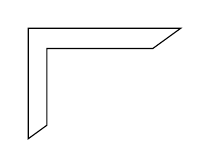
\begin{tikzpicture}[x=0.75pt,y=0.75pt,yscale=-0.75,xscale=0.75] 
\draw   (100,121) -- (198,121) -- (180.06,134) -- (112,134) -- (112,183.31) -- (100,192) -- cycle ;
\end{tikzpicture} },
optionB={
\tikzset{every picture/.style={line width=0.75pt,scale=\scalefactor}} 
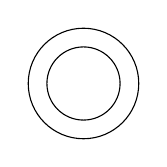
\begin{tikzpicture}[x=0.75pt,y=0.75pt,yscale=-0.75,xscale=0.75]
\draw   (270,45.5) .. controls (270,32.52) and (280.52,22) .. (293.5,22) .. controls (306.48,22) and (317,32.52) .. (317,45.5) .. controls (317,58.48) and (306.48,69) .. (293.5,69) .. controls (280.52,69) and (270,58.48) .. (270,45.5)(258,45.5) .. controls (258,25.89) and (273.89,10) .. (293.5,10) .. controls (313.11,10) and (329,25.89) .. (329,45.5) .. controls (329,65.11) and (313.11,81) .. (293.5,81) .. controls (273.89,81) and (258,65.11) .. (258,45.5) ;
\end{tikzpicture} },
optionC={
\tikzset{every picture/.style={line width=0.75pt,scale=\scalefactor}} 
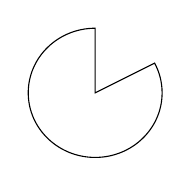
\begin{tikzpicture}[x=0.75pt,y=0.75pt,yscale=-0.75,xscale=0.75]
\draw   (373.19,149.4) .. controls (376.26,155.12) and (378,161.61) .. (378,168.5) .. controls (378,191.42) and (358.75,210) .. (335,210) .. controls (311.25,210) and (292,191.42) .. (292,168.5) .. controls (292,145.58) and (311.25,127) .. (335,127) -- (335,168.5) -- cycle ;
\end{tikzpicture} },
optionD={
\tikzset{every picture/.style={line width=0.75pt,scale=\scalefactor}} 
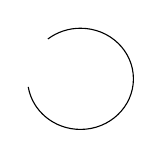
\begin{tikzpicture}[x=0.75pt,y=0.75pt,yscale=-0.75,xscale=0.75] 
\draw  [draw opacity=0] (542.03,145.92) .. controls (547.81,141.58) and (555.09,139) .. (563,139) .. controls (581.78,139) and (597,153.55) .. (597,171.5) .. controls (597,189.45) and (581.78,204) .. (563,204) .. controls (546.07,204) and (532.03,192.17) .. (529.43,176.69) -- (563,171.5) -- cycle ; \draw   (542.03,145.92) .. controls (547.81,141.58) and (555.09,139) .. (563,139) .. controls (581.78,139) and (597,153.55) .. (597,171.5) .. controls (597,189.45) and (581.78,204) .. (563,204) .. controls (546.07,204) and (532.03,192.17) .. (529.43,176.69) ;  
\end{tikzpicture} },
questionTag={C6M11 – DT – Q7}, 
correctoption={D},
}

\begin{minipage}{\linewidth}
\hspace{1cm}
\centering
\tiny
\renewcommand{\arraystretch}{1.25}
\begin{tabular}{|M{1.2cm}|M{0.8cm}|M{0.8cm}|M{0.8cm}|M{0.8cm}|M{0.8cm}|}
\hline
Option & A (\ding{55}) & B (\ding{55}) & C (\ding{55}) & \cellcolor{cellgreen} D (\ding{51}) & E \\ 
\hline
6 A & \highno{0\%} & \highno{0\%} & \highno{0\%} & \highgreen{100\%} & \highno{0\%} \\ 
 \hline 
6 B & \highno{5\%} & \highno{0\%} & \highno{0\%} & \highgreen{89\%} & \highno{5\%} \\ \hline
\end{tabular}
\end{minipage}

\end{frame}
% \input{4. PPT/6. My Answer/Math/C6/117_C6M - Q35}


\begin{frame}[shrink=0.1,label=QPC6QC6M11 - DT - Q4]{Q52\small [4. Basic Geometrical Ideas \& 5 - Understanding Elementary Shapes]}
\vspace{-0.2cm}
\mcqtextbottomOneFour{
questionnumber={52}, 
questiontext={Which teddy bear shows an incorrect measurement of angles?},
optionA={ \adjustbox{scale=\scalefactor}{
\includegraphics[height= 2cm, width=2.8cm]{C6M11 - DT - Q4i.png}}  },
optionB={\adjustbox{scale=\scalefactor}{
\includegraphics[height= 2cm, width=2.8cm]{C6M11 - DT - Q4ii.png}}  },
optionC={\adjustbox{scale=\scalefactor}{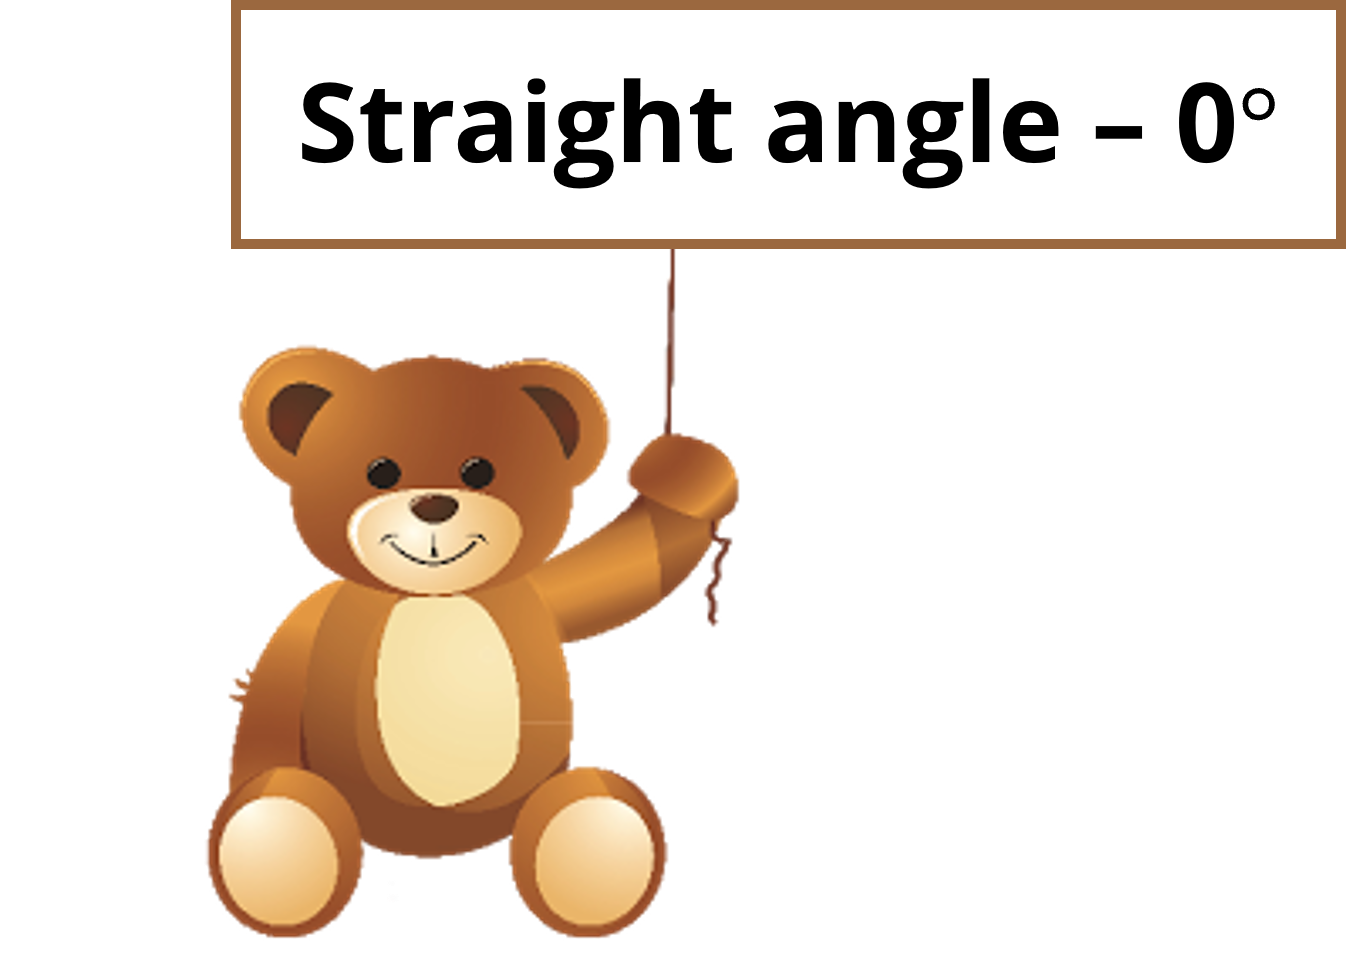
\includegraphics[height= 2cm, width=2.8cm]{C6M11 - DT - Q4iii.png}} },
optionD={ All the above},
questionTag={C6M11 - DT - Q4}, 
correctoption={D},
}

\begin{minipage}{\linewidth}
\hspace{1cm}
\centering
\tiny
\renewcommand{\arraystretch}{1.25}
\begin{tabular}{|M{1.2cm}|M{0.8cm}|M{0.8cm}|M{0.8cm}|M{0.8cm}|M{0.8cm}|}
\hline
Option & A (\ding{55}) & B (\ding{55}) & C (\ding{55}) & \cellcolor{cellgreen} D (\ding{51}) & E \\ 
\hline
6 A & \highno{13\%} & \highno{13\%} & \highno{53\%} & \highred{20\%} & \highno{0\%} \\ 
 \hline 
6 B & \highno{21\%} & \highno{16\%} & \highno{32\%} & \highred{32\%} & \highno{0\%} \\ \hline
\end{tabular}
\end{minipage}

\end{frame}
% \input{4. PPT/6. My Answer/Math/C6/117_C6M - Q52}


\begin{frame}[shrink=0.1,label=QPC6QC6M12 - CT - Q1]{Q58\small [4. Basic Geometrical Ideas \& 5 - Understanding Elementary Shapes]}
\vspace{-0.2cm}
\mcqtextbottomOneFour{
questionnumber={58 - Critical Thinking},
questionTag = {C6M12 - CT - Q1},
questiontext = {Vijay had a square and a rectangular piece of paper. If he tore both the papers diagonally, find the number of triangles formed with three different side lengths.},
optionA={4},
optionB={0},
optionC={3},
optionD={2},
correctoption = {D},
}

\begin{minipage}{\linewidth}
\hspace{1cm}
\centering
\tiny
\renewcommand{\arraystretch}{1.25}
\begin{tabular}{|M{1.2cm}|M{0.8cm}|M{0.8cm}|M{0.8cm}|M{0.8cm}|M{0.8cm}|}
\hline
Option & A (\ding{55}) & B (\ding{55}) & C (\ding{55}) & \cellcolor{cellgreen} D (\ding{51}) & E \\ 
\hline
6 A & \highno{40\%} & \highno{13\%} & \highno{13\%} & \highred{33\%} & \highno{0\%} \\ 
 \hline 
6 B & \highno{5\%} & \highno{11\%} & \highno{74\%} & \highred{5\%} & \highno{5\%} \\ \hline
\end{tabular}
\end{minipage}

\end{frame}
% \input{4. PPT/6. My Answer/Math/C6/117_C6M - Q58 - Critical Thinking}


\begin{frame}[shrink=0.1,label=QPC6QC6M05 - DT - Q4]{Q10 [6. Integers]}
\vspace{-0.2cm}
\mcqtextbottomOneFour{
questionnumber={10}, 
questiontext={Find the greatest integers from the following.},
optionA={$-$123},
optionB={122},
optionC={$-$12},
optionD={0},
questionTag={C6M05 - DT - Q4}, 
correctoption={B},
}

\begin{minipage}{\linewidth}
\hspace{1cm}
\centering
\tiny
\renewcommand{\arraystretch}{1.25}
\begin{tabular}{|M{1.2cm}|M{0.8cm}|M{0.8cm}|M{0.8cm}|M{0.8cm}|M{0.8cm}|}
\hline
Option & A (\ding{55}) & \cellcolor{cellgreen} B (\ding{51}) & C (\ding{55}) & D (\ding{55}) & E \\ 
\hline
6 A & \highno{20\%} & \highgreen{80\%} & \highno{0\%} & \highno{0\%} & \highno{0\%} \\ 
 \hline 
6 B & \highno{5\%} & \highgreen{84\%} & \highno{0\%} & \highno{11\%} & \highno{0\%} \\ \hline
\end{tabular}
\end{minipage}

\end{frame}
% \input{4. PPT/6. My Answer/Math/C6/117_C6M - Q10}


\begin{frame}[shrink=0.1,label=QPC6QC6M05 - DT - Q1]{Q11 [6. Integers]}
\vspace{-0.2cm}
\mcqtextbottomOneFour{
questionnumber={11}, 
questiontext={Find the set of numbers with one natural number, one whole number and one negative integer.},
optionA={1, 2, 3},
optionB={$-$2, 0, $-$1},
optionC={10, 0, $-$1},
optionD={$-$1, 0, 0},
questionTag={C6M05 - DT - Q1}, 
correctoption={C},
}

\begin{minipage}{\linewidth}
\hspace{1cm}
\centering
\tiny
\renewcommand{\arraystretch}{1.25}
\begin{tabular}{|M{1.2cm}|M{0.8cm}|M{0.8cm}|M{0.8cm}|M{0.8cm}|M{0.8cm}|}
\hline
Option & A (\ding{55}) & B (\ding{55}) & \cellcolor{cellgreen} C (\ding{51}) & D (\ding{55}) & E \\ 
\hline
6 A & \highno{13\%} & \highno{0\%} & \highgreen{80\%} & \highno{7\%} & \highno{0\%} \\ 
 \hline 
6 B & \highno{11\%} & \highno{5\%} & \highgreen{79\%} & \highno{5\%} & \highno{0\%} \\ \hline
\end{tabular}
\end{minipage}

\end{frame}
% \input{4. PPT/6. My Answer/Math/C6/117_C6M - Q11}


\begin{frame}[shrink=0.1,label=QPC6QC6M05 - DT - Q6]{Q26 [6. Integers]}
\vspace{-0.2cm}
\mcqtextbottomOneFour{
questionnumber={26}, 
questiontext={Ben participates in a quiz competition. Find the total mark scored by Ben if he got 2 marks for the correct answer and $-$1 mark for the wrong answer.\\
\tikzset{every picture/.style={line width=0.75pt,scale=\scalefactor}} 
\hspace{2cm}
\begin{tikzpicture}[x=0.75pt,y=0.75pt,yscale=-0.75,xscale=0.75] 
\draw (321,73) node  {\adjustbox{scale=\scalefactor}{
\includegraphics[width=219.5pt,height=20pt]{C6M05 - DT - Q6.png}}};
\draw (111,101) node [anchor=north west][inner sep=0.75pt]   [align=left] {$+$2 };
\draw (209,101) node [anchor=north west][inner sep=0.75pt]   [align=left] {\mbox{$-$}1};
\end{tikzpicture}
},
optionA={3},
optionB={$-$6},
optionC={1},
optionD={4},
questionTag={C6M05 - DT - Q6}, 
correctoption={D},
}

\begin{minipage}{\linewidth}
\hspace{1cm}
\centering
\tiny
\renewcommand{\arraystretch}{1.25}
\begin{tabular}{|M{1.2cm}|M{0.8cm}|M{0.8cm}|M{0.8cm}|M{0.8cm}|M{0.8cm}|}
\hline
Option & A (\ding{55}) & B (\ding{55}) & C (\ding{55}) & \cellcolor{cellgreen} D (\ding{51}) & E \\ 
\hline
6 A & \highno{20\%} & \highno{20\%} & \highno{20\%} & \highred{27\%} & \highno{13\%} \\ 
 \hline 
6 B & \highno{16\%} & \highno{16\%} & \highno{26\%} & \highno{42\%} & \highno{0\%} \\ \hline
\end{tabular}
\end{minipage}

\end{frame}
\begin{frame}{Q26 - My Answer Responses}
    \vspace{-0.6cm}
    \begin{multicols}{3}

   

    % Image: Q26_D117157_Math.png - Scaled height: 16.65mm
    \begin{minipage}{\linewidth}
    \RaggedRight\textbf{\tiny \highgreen{Aswin P [D]}} \\ 
    \vspace{4.00pt}\fcolorbox{blue}{white}{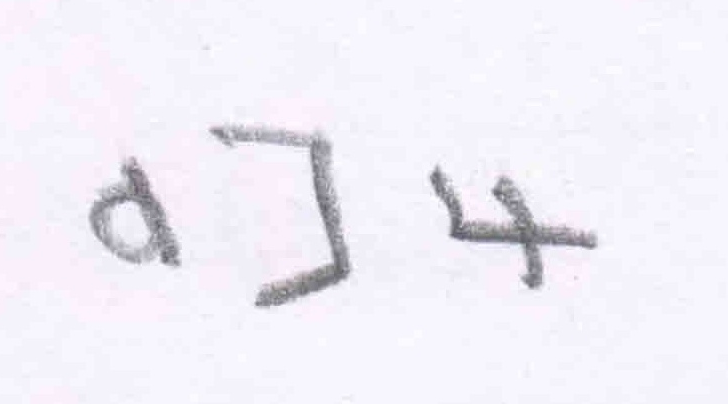
\includegraphics[width=2cm]{Q26_D117157_Math.png}}
    \end{minipage}
    \vspace{10pt}

    % Image: Q26_D117159_Math.png - Scaled height: 24.18mm
    \begin{minipage}{\linewidth}
    \RaggedRight\textbf{\tiny \highred{Gurunathan K R [B]}} \\ 
    \vspace{4.00pt}\fcolorbox{blue}{white}{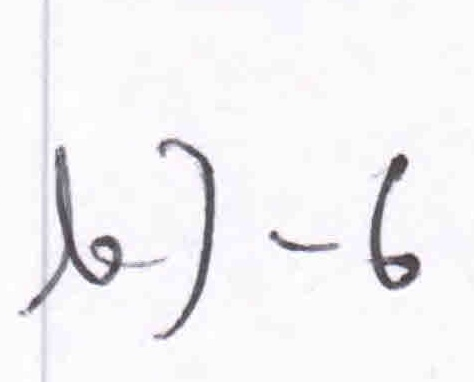
\includegraphics[width=2cm]{Q26_D117159_Math.png}}
    \end{minipage}
    \vspace{10pt}

    % Image: Q26_D117161_Math.png - Scaled height: 20.83mm
    \begin{minipage}{\linewidth}
    \RaggedRight\textbf{\tiny \highgreen{Kiruthik D [D]}} \\ 
    \vspace{4.00pt}\fcolorbox{blue}{white}{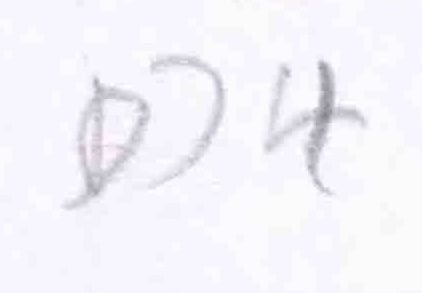
\includegraphics[width=2cm]{Q26_D117161_Math.png}}
    \end{minipage}
    \vspace{10pt}

    % Image: Q26_D117163_Math.png - Scaled height: 14.85mm
    \begin{minipage}{\linewidth}
    \RaggedRight\textbf{\tiny \highred{Manjunath A [A]}} \\ 
    \vspace{4.00pt}\fcolorbox{blue}{white}{
\includegraphics[width=2cm]{Q26_D117163_Math.png}}
    \end{minipage}
    \vspace{10pt}

     % Image: Q26_D117135_Math.png - Scaled height: 8.68mm
    \begin{minipage}{\linewidth}
    \RaggedRight\textbf{\tiny \highgreen{Dheeresh J A [D]}} \\ 
    \vspace{4.00pt}\fcolorbox{blue}{white}{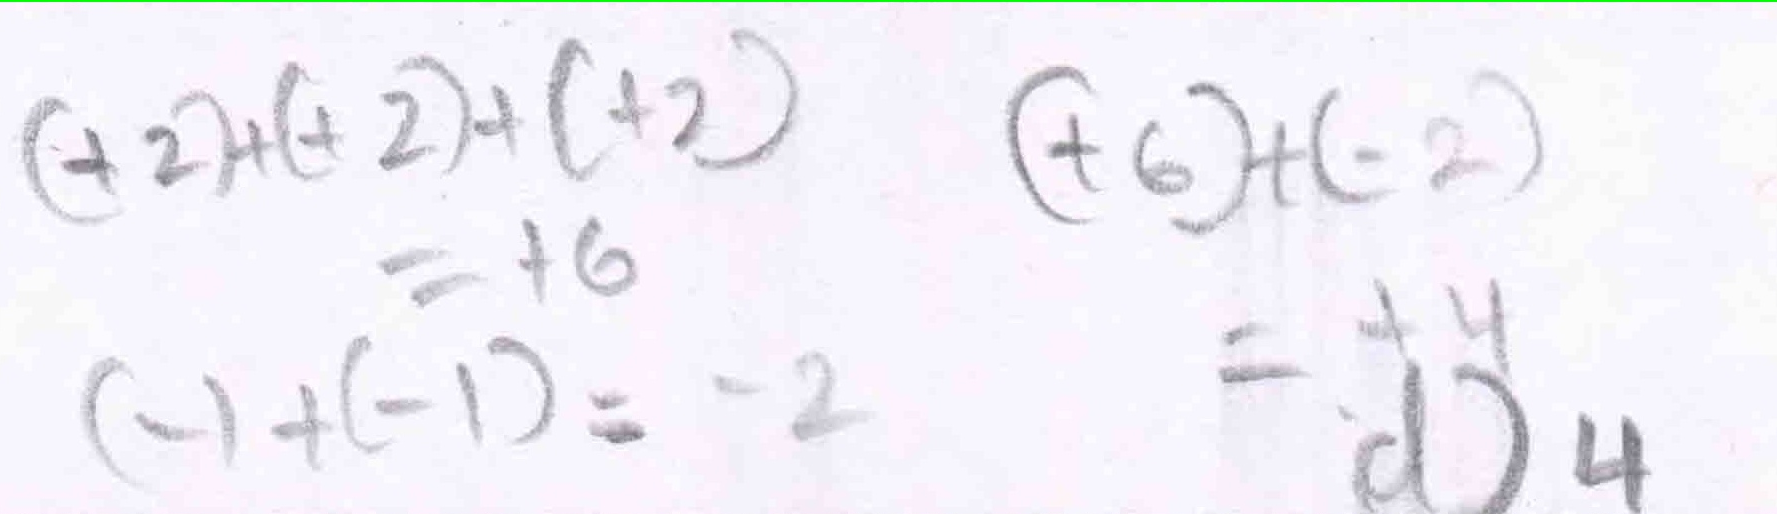
\includegraphics[width=4cm]{Q26_D117135_Math.png}}
    \end{minipage}
    \vspace{10pt}

    % Image: Q26_D117167_Math.png - Scaled height: 4.09mm
    \begin{minipage}{\linewidth}
    \RaggedRight\textbf{\tiny \highgreen{Sriram Karthikeyan V [D]}} \\ 
    \vspace{4.00pt}\fcolorbox{blue}{white}{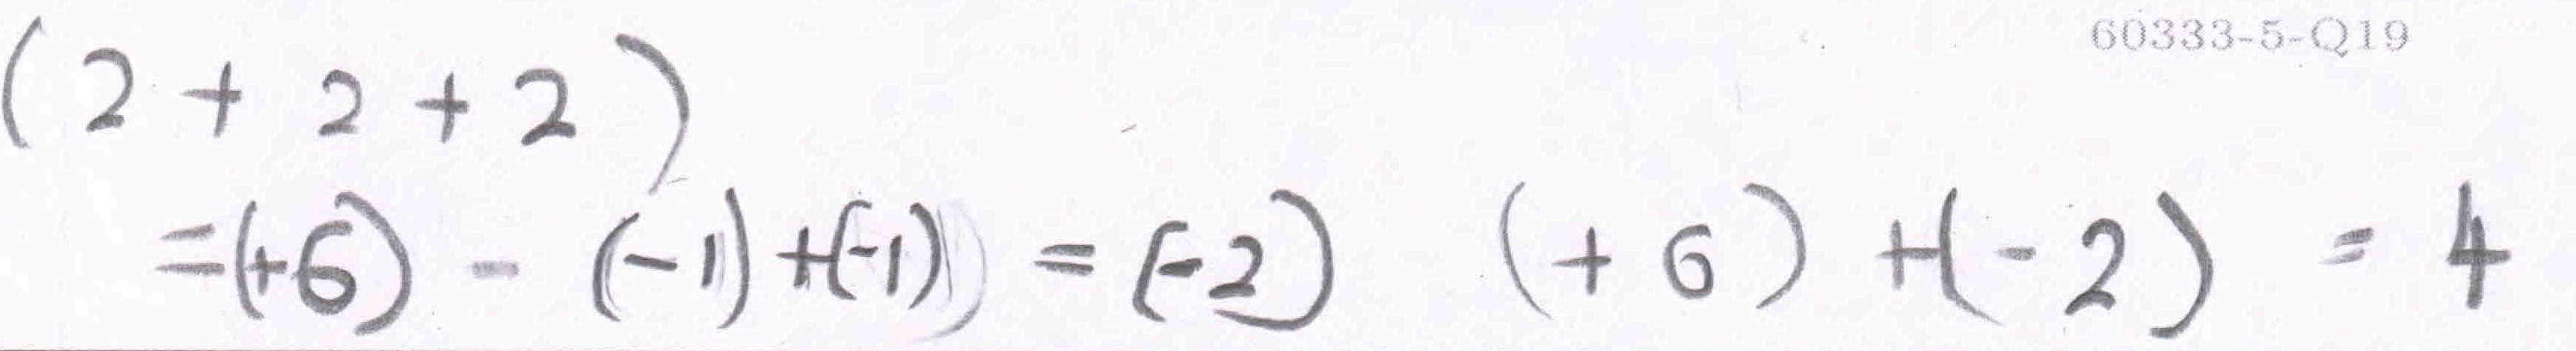
\includegraphics[width=4cm]{Q26_D117167_Math.png}}
    \end{minipage}
    \vspace{10pt}

    % Image: Q26_D117171_Math.png - Scaled height: 7.51mm
    \begin{minipage}{\linewidth}
    \RaggedRight\textbf{\tiny \highgreen{Elakyaa N [D]}} \\ 
    \vspace{4.00pt}\fcolorbox{blue}{white}{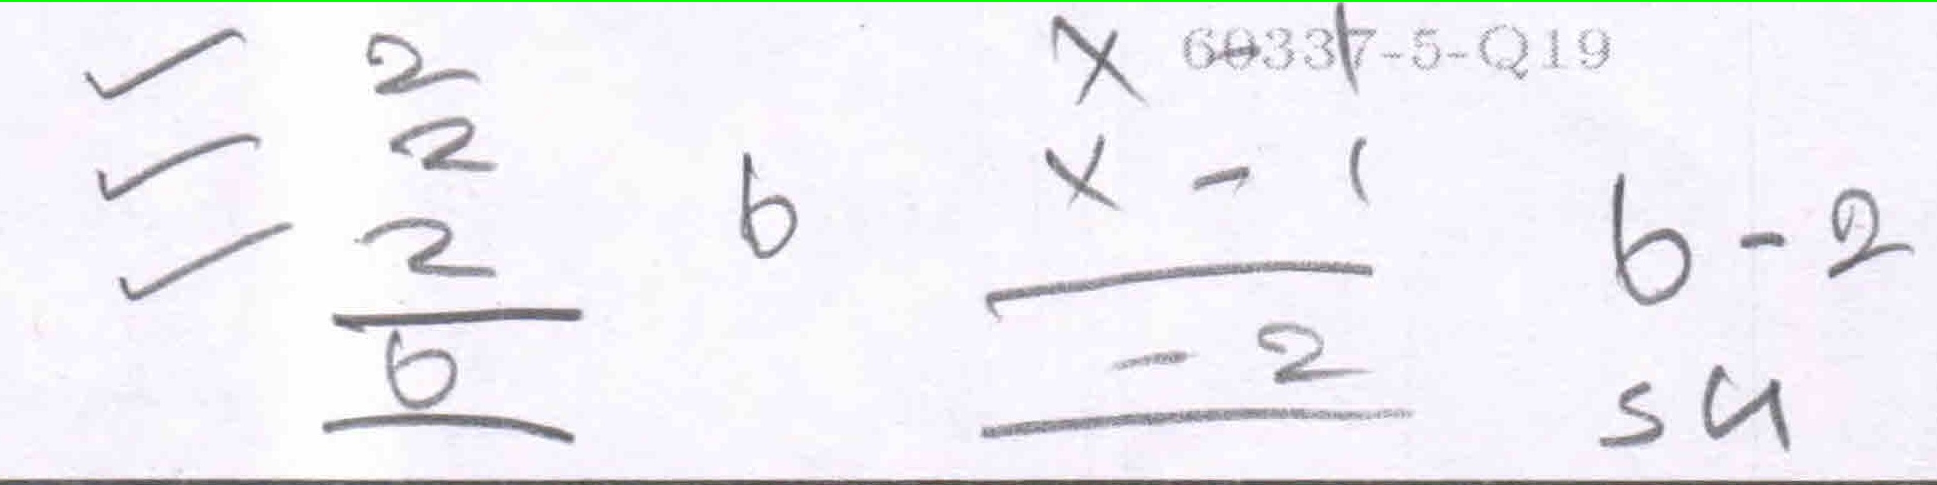
\includegraphics[width=4cm]{Q26_D117171_Math.png}}
    \end{minipage}
    \vspace{10pt}

    \end{multicols}
\end{frame}




\begin{frame}[shrink=0.1,label=QPC6QC6M05 - DT - Q2]{Q34 [6. Integers]}
\vspace{-0.2cm}
\mcqtextbottomOneFour{
questionnumber={34}, 
questiontext={A squirrel jumps 3 points to the left side of the number line. Find the position of the squirrel in the number line.\\
\tikzset{every picture/.style={line width=0.75pt,scale=\scalefactor}} 
\hspace{2cm}
\begin{tikzpicture}[x=0.75pt,y=0.75pt,yscale=-1,xscale=1]
\draw (382,82.5) node  {\adjustbox{scale=\scalefactor}{
\includegraphics[width=35pt,height=40pt]{C6M05 - DT - Q2.png}}};
\draw    (154,110.01) -- (569,110.99) (192.02,101.6) -- (191.98,118.6)(230.02,101.69) -- (229.98,118.69)(268.02,101.78) -- (267.98,118.78)(306.02,101.87) -- (305.98,118.87)(344.02,101.96) -- (343.98,118.96)(382.02,102.05) -- (381.98,119.05)(420.02,102.14) -- (419.98,119.14)(458.02,102.23) -- (457.98,119.23)(496.02,102.32) -- (495.98,119.32)(534.02,102.41) -- (533.98,119.41) ;
\draw [shift={(572,111)}, rotate = 180.14] [fill={rgb, 255:red, 0; green, 0; blue, 0 }  ][line width=0.08]  [draw opacity=0] (10.72,-5.15) -- (0,0) -- (10.72,5.15) -- (7.12,0) -- cycle    ;
\draw [shift={(151,110)}, rotate = 0.14] [fill={rgb, 255:red, 0; green, 0; blue, 0 }  ][line width=0.08]  [draw opacity=0] (10.72,-5.15) -- (0,0) -- (10.72,5.15) -- (7.12,0) -- cycle    ;
\draw (378,123) node [anchor=north west][inner sep=0.75pt]   [align=left] {0};
\end{tikzpicture}
},
optionA={+3},
optionB={$-$3},
optionC={$-$6},
optionD={+6},
questionTag={C6M05 - DT - Q2}, 
correctoption={B},
}

\begin{minipage}{\linewidth}
\hspace{1cm}
\centering
\tiny
\renewcommand{\arraystretch}{1.25}
\begin{tabular}{|M{1.2cm}|M{0.8cm}|M{0.8cm}|M{0.8cm}|M{0.8cm}|M{0.8cm}|}
\hline
Option & A (\ding{55}) & \cellcolor{cellgreen} B (\ding{51}) & C (\ding{55}) & D (\ding{55}) & E \\ 
\hline
6 A & \highno{0\%} & \highgreen{93\%} & \highno{0\%} & \highno{7\%} & \highno{0\%} \\ 
 \hline 
6 B & \highno{16\%} & \highgreen{79\%} & \highno{0\%} & \highno{0\%} & \highno{5\%} \\ \hline
\end{tabular}
\end{minipage}

\end{frame}
% \input{4. PPT/6. My Answer/Math/C6/117_C6M - Q34}


\begin{frame}[shrink=0.1,label=QPC6QC6M05 - DT - Q5]{Q56 [6. Integers]}
\vspace{-0.2cm}
\mcqtextbottomOneFour{
questionnumber={56}, 
questiontext={Find the correct option.},
optionA={$-$3 $+$ ($-$3) = $-$6},
optionB={$-$3 $+$ 3 = $-$6},
optionC={ $-$3 $-$ 3 = 0},
optionD={3 $-$ 3 = 6 },
questionTag={C6M05 - DT - Q5}, 
correctoption={A},
}

\begin{minipage}{\linewidth}
\hspace{1cm}
\centering
\tiny
\renewcommand{\arraystretch}{1.25}
\begin{tabular}{|M{1.2cm}|M{0.8cm}|M{0.8cm}|M{0.8cm}|M{0.8cm}|M{0.8cm}|}
\hline
Option & \cellcolor{cellgreen} A (\ding{51}) & B (\ding{55}) & C (\ding{55}) & D (\ding{55}) & E \\ 
\hline
6 A & \highgreen{80\%} & \highno{0\%} & \highno{13\%} & \highno{0\%} & \highno{7\%} \\ 
 \hline 
6 B & \highno{47\%} & \highno{21\%} & \highno{16\%} & \highno{16\%} & \highno{0\%} \\ \hline
\end{tabular}
\end{minipage}

\end{frame}
\begin{frame}{Q56 - My Answer Responses}
    \vspace{-0.6cm}
    \begin{multicols}{2}

    % Image: Q56_D117135_Math.png - Scaled height: 3.99mm
    \begin{minipage}{\linewidth}
    \RaggedRight\textbf{\tiny \highgreen{Dheeresh J A [A]}} \\ 
    \vspace{4.00pt}\fcolorbox{blue}{white}{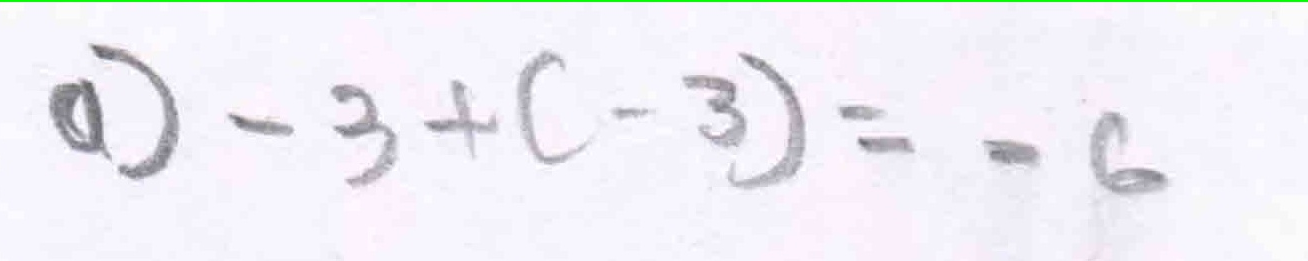
\includegraphics[width=3cm]{Q56_D117135_Math.png}}
    \end{minipage}
    \vspace{10pt}

    % Image: Q56_D117151_Math.png - Scaled height: 3.65mm
    \begin{minipage}{\linewidth}
    \RaggedRight\textbf{\tiny \highgreen{Karnika R [A]}} \\ 
    \vspace{4.00pt}\fcolorbox{blue}{white}{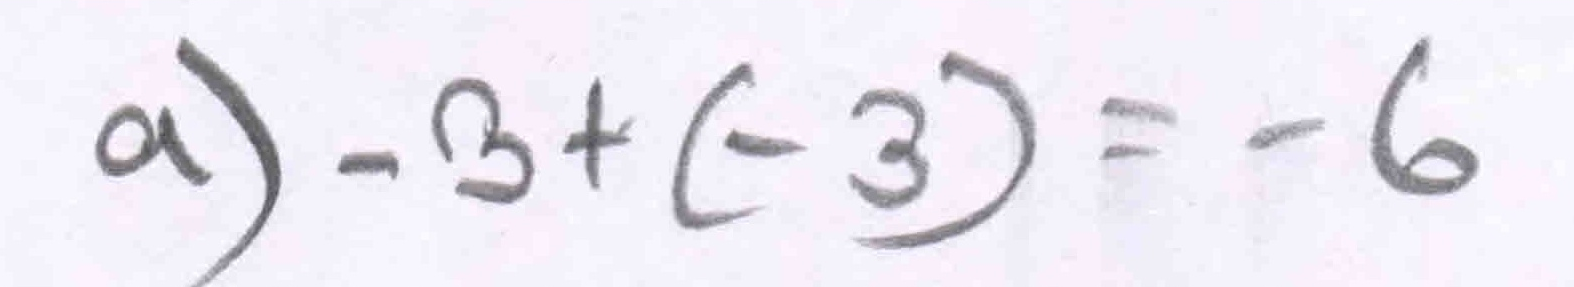
\includegraphics[width=3cm]{Q56_D117151_Math.png}}
    \end{minipage}
    \vspace{10pt}

    % Image: Q56_D117153_Math.png - Scaled height: 4.41mm
    \begin{minipage}{\linewidth}
    \RaggedRight\textbf{\tiny \highred{Priyadharshini S A [C]}} \\ 
    \vspace{4.00pt}\fcolorbox{blue}{white}{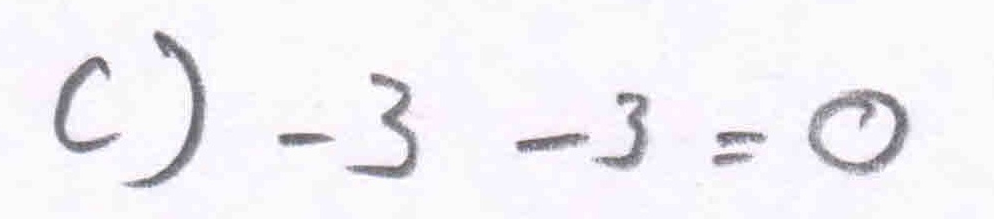
\includegraphics[width=3cm]{Q56_D117153_Math.png}}
    \end{minipage}
    \vspace{10pt}

    % Image: Q56_D117157_Math.png - Scaled height: 3.06mm
    \begin{minipage}{\linewidth}
    \RaggedRight\textbf{\tiny \highgreen{Aswin P [A]}} \\ 
    \vspace{4.00pt}\fcolorbox{blue}{white}{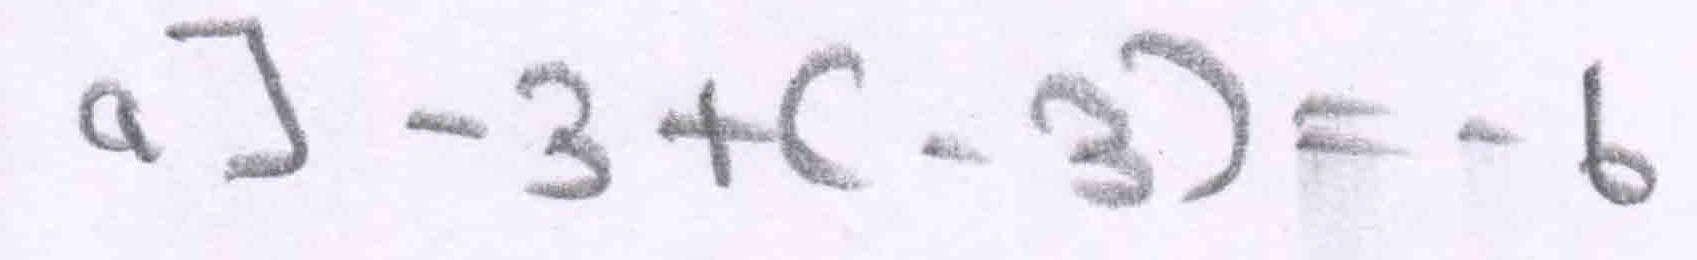
\includegraphics[width=3cm]{Q56_D117157_Math.png}}
    \end{minipage}
    \vspace{10pt}

    % Image: Q56_D117163_Math.png - Scaled height: 2.97mm
    \begin{minipage}{\linewidth}
    \RaggedRight\textbf{\tiny \highgreen{Manjunath A [A]}} \\ 
    \vspace{4.00pt}\fcolorbox{blue}{white}{
\includegraphics[width=3cm]{Q56_D117163_Math.png}}
    \end{minipage}
    \vspace{10pt}

    \end{multicols}
\end{frame}




\begin{frame}[shrink=0.1,label=QPC6QC6M06 - DT - Q10]{Q8 [7. Fractions]}
\vspace{-0.2cm}
\mcqtextbottomOneFour{
questionnumber={8}, 
questionTag={C6M06 - DT - Q10}, 
questiontext={Add:  {{$\dfrac{2}{15}$}} + {{$\dfrac{1}{5}$}}.},
optionA={ {{$\dfrac{3}{20}$}} },
optionB={ {{$\dfrac{5}{15}$}} },
optionC={ {{$\dfrac{1}{5}$}} },
optionD={ {{$\dfrac{21}{5}$}} },
correctoption={B},
}

\begin{minipage}{\linewidth}
\hspace{1cm}
\centering
\tiny
\renewcommand{\arraystretch}{1.25}
\begin{tabular}{|M{1.2cm}|M{0.8cm}|M{0.8cm}|M{0.8cm}|M{0.8cm}|M{0.8cm}|}
\hline
Option & A (\ding{55}) & \cellcolor{cellgreen} B (\ding{51}) & C (\ding{55}) & D (\ding{55}) & E \\ 
\hline
6 A & \highno{7\%} & \highgreen{80\%} & \highno{13\%} & \highno{0\%} & \highno{0\%} \\ 
 \hline 
6 B & \highno{42\%} & \highno{53\%} & \highno{5\%} & \highno{0\%} & \highno{0\%} \\ \hline
\end{tabular}
\end{minipage}

\end{frame}
\begin{frame}{Q8 - My Answer Responses}
    \vspace{-0.6cm}
    \begin{multicols}{4}

    % Image: Q8_D117146_Math.png - Scaled height: 4.13mm
    \begin{minipage}{\linewidth}
    \RaggedRight\textbf{\tiny \highgreen{Aashinisri G [B]}} \\ 
    \vspace{4.00pt}\fcolorbox{blue}{white}{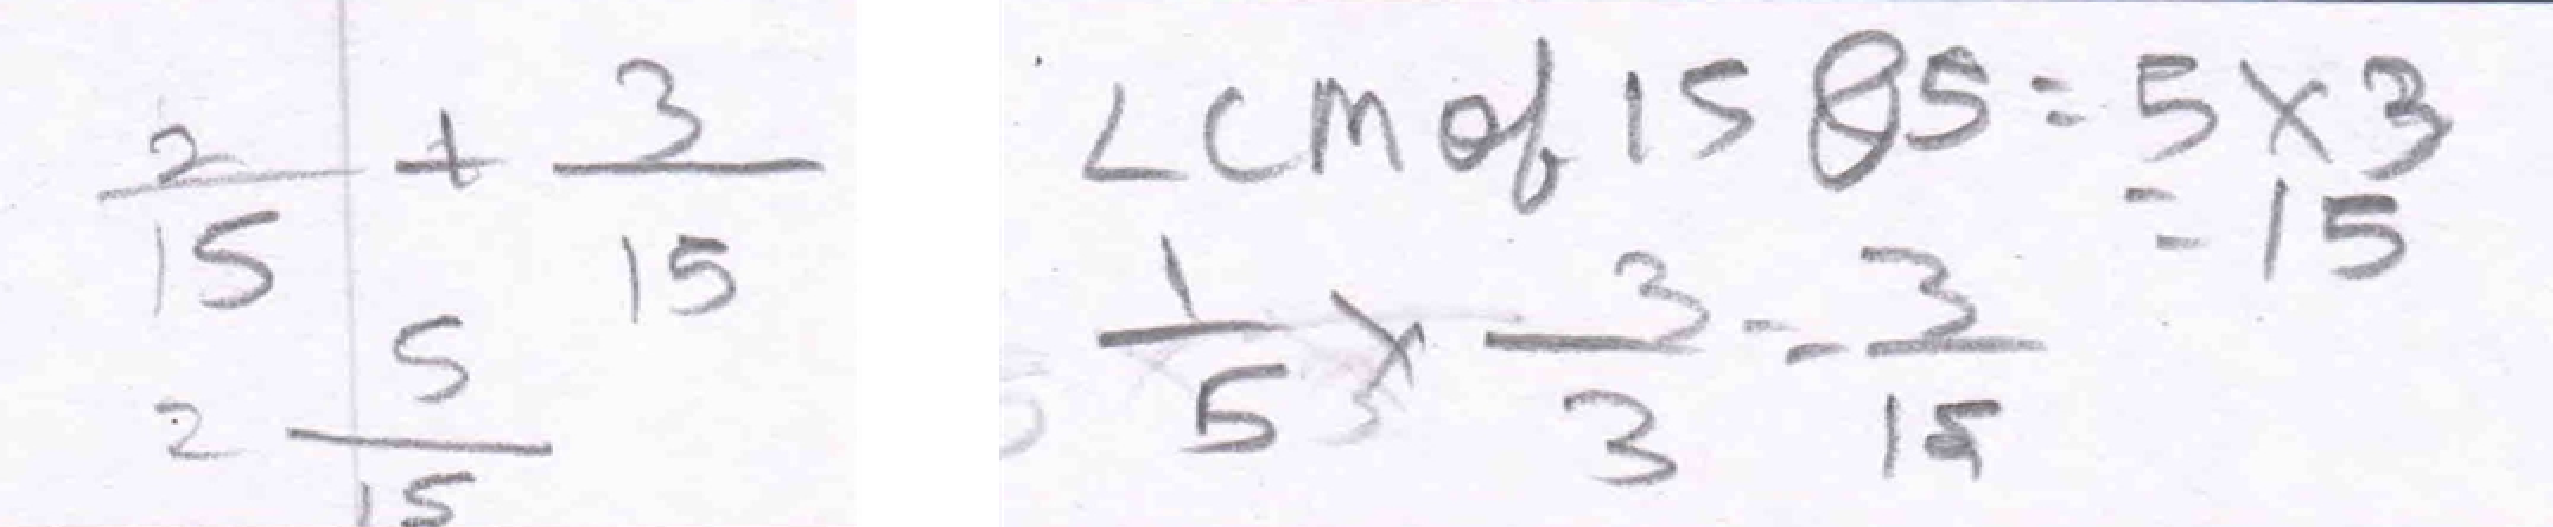
\includegraphics[width=3cm]{Q8_D117146_Math.png}}
    \end{minipage}
    \vspace{10pt}

    % Image: Q8_D117147_Math.png - Scaled height: 2.30mm
    \begin{minipage}{\linewidth}
    \RaggedRight\textbf{\tiny \highgreen{Anusika M [B]}} \\ 
    \vspace{4.00pt}\fcolorbox{blue}{white}{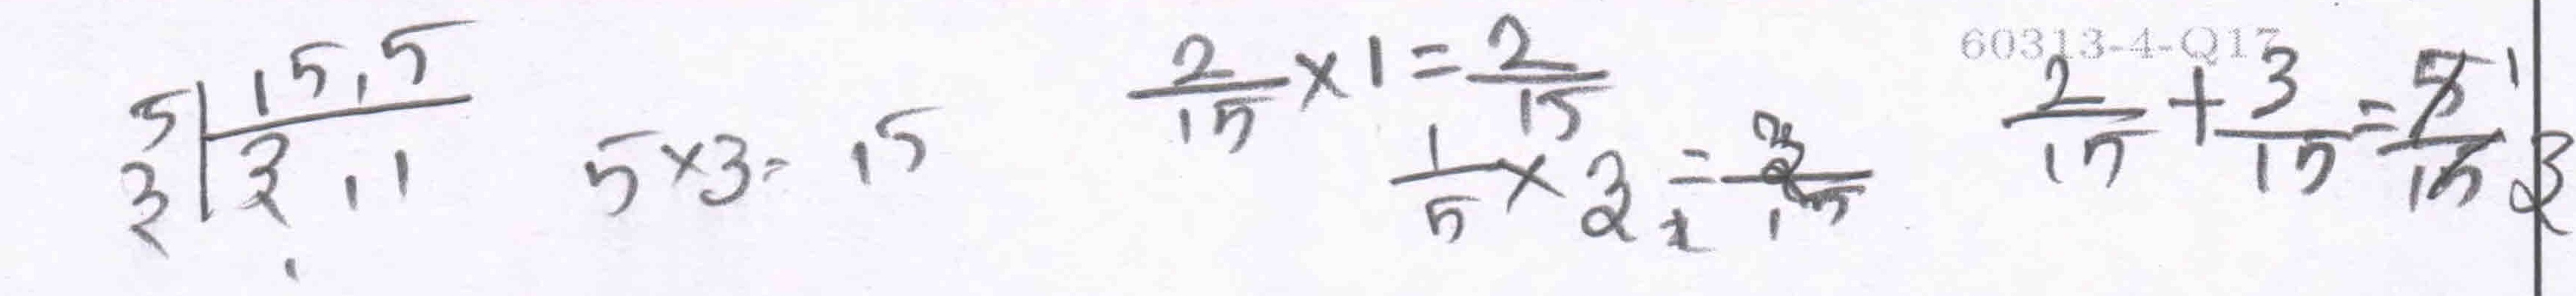
\includegraphics[width=3cm]{Q8_D117147_Math.png}}
    \end{minipage}
    \vspace{10pt}

    % Image: Q8_D117151_Math.png - Scaled height: 16.01mm
    \begin{minipage}{\linewidth}
    \RaggedRight\textbf{\tiny \highred{Karnika R [C]}} \\ 
    \vspace{4.00pt}\fcolorbox{blue}{white}{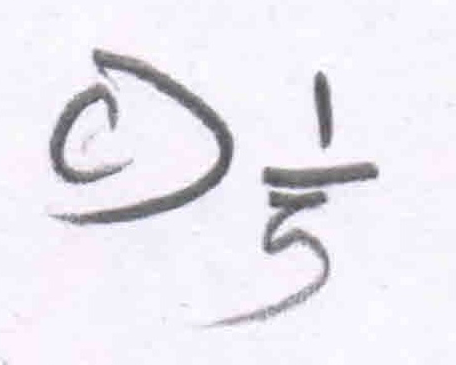
\includegraphics[width=1cm]{Q8_D117151_Math.png}}
    \end{minipage}
    \vspace{10pt}

    % Image: Q8_D117153_Math.png - Scaled height: 19.11mm
    \begin{minipage}{\linewidth}
    \RaggedRight\textbf{\tiny \highgreen{Priyadharshini S A [B]}} \\ 
    \vspace{4.00pt}\fcolorbox{blue}{white}{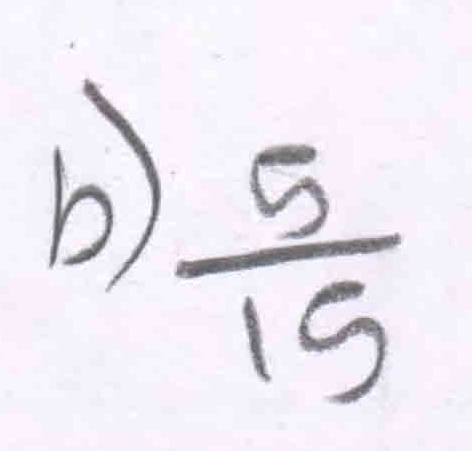
\includegraphics[width=1cm]{Q8_D117153_Math.png}}
    \end{minipage}
    \vspace{10pt}

    % Image: Q8_D117157_Math.png - Scaled height: 3.38mm
    \begin{minipage}{\linewidth}
    \RaggedRight\textbf{\tiny \highgreen{Aswin P [B]}} \\ 
    \vspace{4.00pt}\fcolorbox{blue}{white}{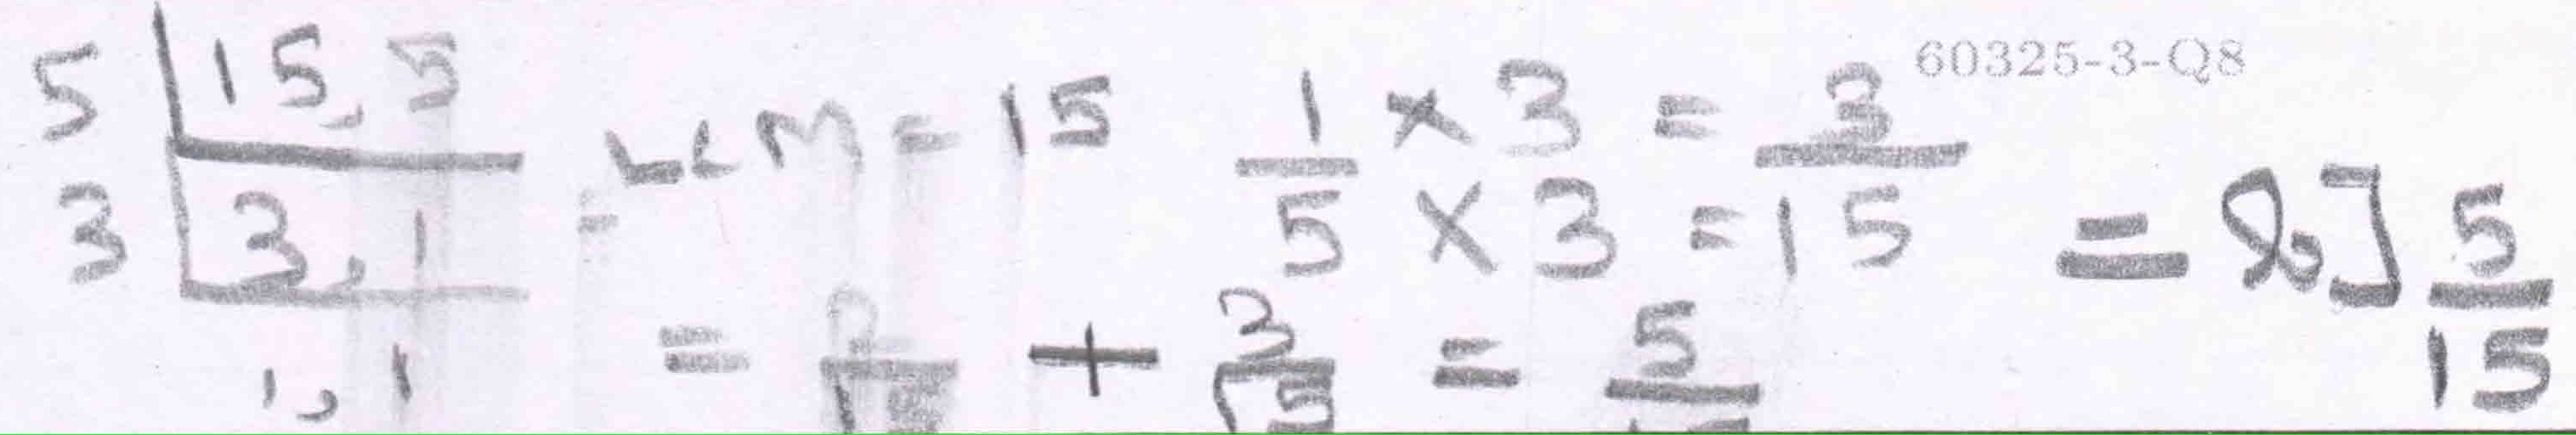
\includegraphics[width=3cm]{Q8_D117157_Math.png}}
    \end{minipage}
    \vspace{10pt}

    % Image: Q8_D117159_Math.png - Scaled height: 14.37mm
    \begin{minipage}{\linewidth}
    \RaggedRight\textbf{\tiny \highred{Gurunathan K R [A]}} \\ 
    \vspace{4.00pt}\fcolorbox{blue}{white}{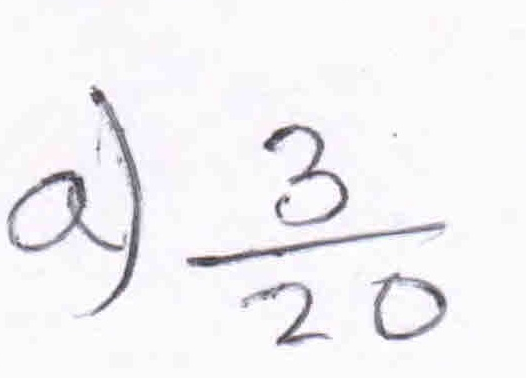
\includegraphics[width=2cm]{Q8_D117159_Math.png}}
    \end{minipage}
    \vspace{10pt}

    % Image: Q8_D117161_Math.png - Scaled height: 13.33mm
    \begin{minipage}{\linewidth}
    \RaggedRight\textbf{\tiny \highred{Kiruthik D [A]}} \\ 
    \vspace{4.00pt}\fcolorbox{blue}{white}{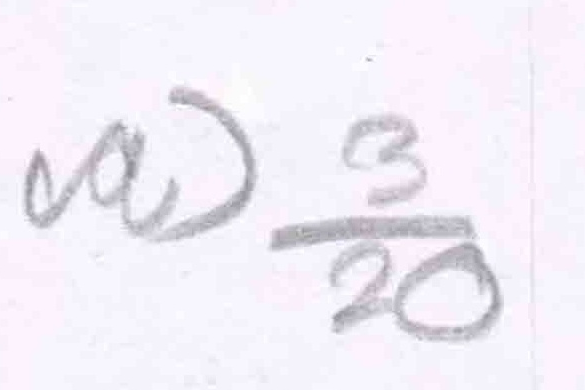
\includegraphics[width=2cm]{Q8_D117161_Math.png}}
    \end{minipage}
    \vspace{10pt}

    % Image: Q8_D117163_Math.png - Scaled height: 9.52mm
    \begin{minipage}{\linewidth}
    \RaggedRight\textbf{\tiny \highgreen{Manjunath A [B]}} \\ 
    \vspace{4.00pt}\fcolorbox{blue}{white}{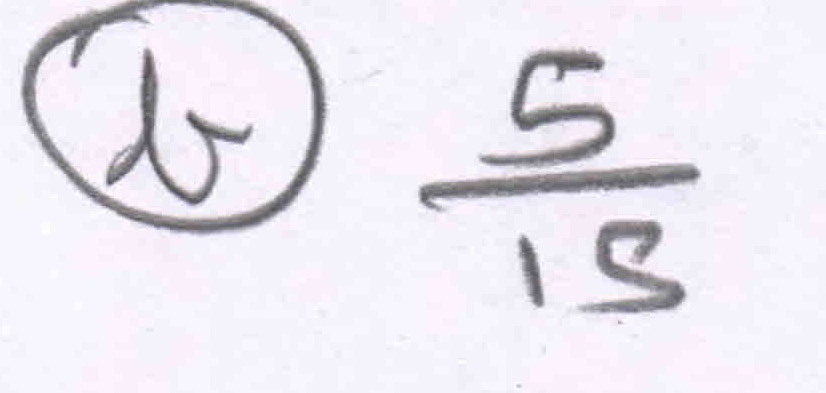
\includegraphics[width=2cm]{Q8_D117163_Math.png}}
    \end{minipage}
    \vspace{10pt}

    % Image: Q8_D117164_Math.png - Scaled height: 11.70mm
    \begin{minipage}{\linewidth}
    \RaggedRight\textbf{\tiny \highred{Nithin N [A]}} \\ 
    \vspace{4.00pt}\fcolorbox{blue}{white}{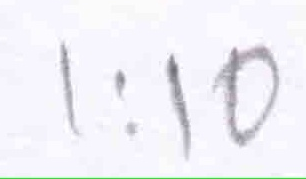
\includegraphics[width=2cm]{Q8_D117164_Math.png}}
    \end{minipage}
    \vspace{10pt}

    % Image: Q8_D117167_Math.png - Scaled height: 2.92mm
    \begin{minipage}{\linewidth}
    \RaggedRight\textbf{\tiny \highgreen{Sriram Karthikeyan V [B]}} \\ 
    \vspace{4.00pt}\fcolorbox{blue}{white}{\includegraphics[width=3cm]{Q8_D117167_Math.png}}
    \end{minipage}
    \vspace{10pt}

    \end{multicols}
\end{frame}




\begin{frame}[shrink=0.1,label=QPC6QC6M06 - DT - Q4]{Q30 [7. Fractions]}
\vspace{-0.2cm}
\mcqtextbottomTwoTwo{
questionnumber={30}, 
questionTag={C6M06 - DT - Q4}, 
questiontext={Find the correct representation of {{$\dfrac{3}{5}$}} in the given number lines.},
optionA={\tikzset{every picture/.style={line width=0.75pt,scale=\scalefactor}} 
\begin{tikzpicture}[x=0.75pt,y=0.75pt,yscale=-1,xscale=1]
\draw    (112,72) -- (398,72) (150,63.5) -- (150,80.5)(188,63.5) -- (188,80.5)(226,63.5) -- (226,80.5)(264,63.5) -- (264,80.5)(302,63.5) -- (302,80.5)(340,63.5) -- (340,80.5)(378,63.5) -- (378,80.5) ;
\draw [shift={(400,72)}, rotate = 180] [color={rgb, 255:red, 0; green, 0; blue, 0 }  ][line width=0.75]    (10.93,-4.9) .. controls (6.95,-2.3) and (3.31,-0.67) .. (0,0) .. controls (3.31,0.67) and (6.95,2.3) .. (10.93,4.9)   ;
\draw [shift={(110,72)}, rotate = 0] [color={rgb, 255:red, 0; green, 0; blue, 0 }  ][line width=0.75]    (10.93,-4.9) .. controls (6.95,-2.3) and (3.31,-0.67) .. (0,0) .. controls (3.31,0.67) and (6.95,2.3) .. (10.93,4.9)   ;
\draw (180,84) node [anchor=north west][inner sep=0.75pt]   [align=left] {{{$\dfrac{3}{5}$}}};
\draw (373,84) node [anchor=north west][inner sep=0.75pt]   [align=left] {1};
\draw (145.24,84) node [anchor=north west][inner sep=0.75pt]   [align=left] {0};
\end{tikzpicture} },
optionB={\tikzset{every picture/.style={line width=0.75pt,scale=\scalefactor}} 
\begin{tikzpicture}[x=0.75pt,y=0.75pt,yscale=-1,xscale=1]
\draw    (112,72) -- (398,72) (150,63.5) -- (150,80.5)(188,63.5) -- (188,80.5)(226,63.5) -- (226,80.5)(264,63.5) -- (264,80.5)(302,63.5) -- (302,80.5)(340,63.5) -- (340,80.5)(378,63.5) -- (378,80.5) ;
\draw [shift={(400,72)}, rotate = 180] [color={rgb, 255:red, 0; green, 0; blue, 0 }  ][line width=0.75]    (10.93,-4.9) .. controls (6.95,-2.3) and (3.31,-0.67) .. (0,0) .. controls (3.31,0.67) and (6.95,2.3) .. (10.93,4.9)   ;
\draw [shift={(110,72)}, rotate = 0] [color={rgb, 255:red, 0; green, 0; blue, 0 }  ][line width=0.75]    (10.93,-4.9) .. controls (6.95,-2.3) and (3.31,-0.67) .. (0,0) .. controls (3.31,0.67) and (6.95,2.3) .. (10.93,4.9)   ;
\draw (335,84) node [anchor=north west][inner sep=0.75pt]   [align=left] {{{$\dfrac{3}{5}$}}};
\draw (145.24,84) node [anchor=north west][inner sep=0.75pt]   [align=left] {0};
\draw (373,84) node [anchor=north west][inner sep=0.75pt]   [align=left] {1};
\end{tikzpicture}},
optionC={\tikzset{every picture/.style={line width=0.75pt,scale=\scalefactor}} 
\begin{tikzpicture}[x=0.75pt,y=0.75pt,yscale=-1,xscale=1]
\draw    (112,72) -- (398,72) (150,63.5) -- (150,80.5)(188,63.5) -- (188,80.5)(226,63.5) -- (226,80.5)(264,63.5) -- (264,80.5)(302,63.5) -- (302,80.5)(340,63.5) -- (340,80.5)(378,63.5) -- (378,80.5) ;
\draw [shift={(400,72)}, rotate = 180] [color={rgb, 255:red, 0; green, 0; blue, 0 }  ][line width=0.75]    (10.93,-4.9) .. controls (6.95,-2.3) and (3.31,-0.67) .. (0,0) .. controls (3.31,0.67) and (6.95,2.3) .. (10.93,4.9)   ;
\draw [shift={(110,72)}, rotate = 0] [color={rgb, 255:red, 0; green, 0; blue, 0 }  ][line width=0.75]    (10.93,-4.9) .. controls (6.95,-2.3) and (3.31,-0.67) .. (0,0) .. controls (3.31,0.67) and (6.95,2.3) .. (10.93,4.9)   ;
\draw (218,84) node [anchor=north west][inner sep=0.75pt]   [align=left] {{{$\dfrac{3}{5}$}}};
\draw (180,84) node [anchor=north west][inner sep=0.75pt]   [align=left] {0};
\draw (373,84) node [anchor=north west][inner sep=0.75pt]   [align=left] {1};
\end{tikzpicture}},
optionD={
\tikzset{every picture/.style={line width=0.75pt,scale=\scalefactor}} 
\begin{tikzpicture}[x=0.75pt,y=0.75pt,yscale=-1,xscale=1]
\draw    (112,72) -- (398,72) (150,63.5) -- (150,80.5)(188,63.5) -- (188,80.5)(226,63.5) -- (226,80.5)(264,63.5) -- (264,80.5)(302,63.5) -- (302,80.5)(340,63.5) -- (340,80.5)(378,63.5) -- (378,80.5) ;
\draw [shift={(400,72)}, rotate = 180] [color={rgb, 255:red, 0; green, 0; blue, 0 }  ][line width=0.75]    (10.93,-4.9) .. controls (6.95,-2.3) and (3.31,-0.67) .. (0,0) .. controls (3.31,0.67) and (6.95,2.3) .. (10.93,4.9)   ;
\draw [shift={(110,72)}, rotate = 0] [color={rgb, 255:red, 0; green, 0; blue, 0 }  ][line width=0.75]    (10.93,-4.9) .. controls (6.95,-2.3) and (3.31,-0.67) .. (0,0) .. controls (3.31,0.67) and (6.95,2.3) .. (10.93,4.9)   ;
\draw (258,84) node [anchor=north west][inner sep=0.75pt]   [align=left] {{{$\dfrac{3}{5}$}}};
\draw (145.24,84) node [anchor=north west][inner sep=0.75pt]   [align=left] {0};
\draw (333,84) node [anchor=north west][inner sep=0.75pt]   [align=left] {1};
\end{tikzpicture} },
correctoption={D},
}

\begin{minipage}{\linewidth}
\hspace{1cm}
\centering
\tiny
\renewcommand{\arraystretch}{1.25}
\begin{tabular}{|M{1.2cm}|M{0.8cm}|M{0.8cm}|M{0.8cm}|M{0.8cm}|M{0.8cm}|}
\hline
Option & A (\ding{55}) & B (\ding{55}) & C (\ding{55}) & \cellcolor{cellgreen} D (\ding{51}) & E \\ 
\hline
6 A & \highno{7\%} & \highno{33\%} & \highno{0\%} & \highno{60\%} & \highno{0\%} \\ 
 \hline 
6 B & \highno{5\%} & \highno{11\%} & \highno{21\%} & \highno{63\%} & \highno{0\%} \\ \hline
\end{tabular}
\end{minipage}

\end{frame}
% \input{4. PPT/6. My Answer/Math/C6/117_C6M - Q30}


\begin{frame}[shrink=0.1,label=QPC6QC6M06 - DT - Q11]{Q32 [7. Fractions]}
\vspace{-0.2cm}
\mcqtextsideFourOne{
questionnumber={32}, 
questionTag={C6M06 - DT - Q11}, 
questiontext={\\ \medskip
Shalu said {{$\dfrac{2}{5}$}} $-$ {{$\dfrac{1}{5}$}}  is {{$\dfrac{1}{5}$}} \\ \smallskip
Ramu said {{$\dfrac{5}{4}$}} $-$ {{$\dfrac{1}{2}$}} is {{$\dfrac{3}{4}$}} \\ \smallskip
Find whose statement is correct.},
optionA={Shalu’s statement},
optionB={Ramu's statement},
optionC={Both statements are true},
optionD={None of the above},
correctoption={C},
leftmini = {0.5},
rightmini = {0.4},
}

\begin{minipage}{\linewidth}
\hspace{1cm}
\centering
\tiny
\renewcommand{\arraystretch}{1.25}
\begin{tabular}{|M{1.2cm}|M{0.8cm}|M{0.8cm}|M{0.8cm}|M{0.8cm}|M{0.8cm}|}
\hline
Option & A (\ding{55}) & B (\ding{55}) & \cellcolor{cellgreen} C (\ding{51}) & D (\ding{55}) & E \\ 
\hline
6 A & \highno{33\%} & \highno{13\%} & \highno{53\%} & \highno{0\%} & \highno{0\%} \\ 
 \hline 
6 B & \highno{37\%} & \highno{16\%} & \highred{32\%} & \highno{11\%} & \highno{5\%} \\ \hline
\end{tabular}
\end{minipage}

\end{frame}
\begin{frame}{Q32 - My Answer Responses}
    \vspace{-0.6cm}
    \begin{multicols}{3}

    % Image: Q32_D117135_Math.png - Scaled height: 3.86mm
    \begin{minipage}{\linewidth}
    \RaggedRight\textbf{\tiny \highgreen{Dheeresh J A [C]}} \\ 
    \vspace{4.00pt}\fcolorbox{blue}{white}{\includegraphics[width=4cm]{Q32_D117135_Math.png}}
    \end{minipage}
    \vspace{10pt}

    % Image: Q32_D117151_Math.png - Scaled height: 10.70mm
    \begin{minipage}{\linewidth}
    \RaggedRight\textbf{\tiny \highgreen{Karnika R [C]}} \\ 
    \vspace{4.00pt}\fcolorbox{blue}{white}{\includegraphics[width=4cm]{Q32_D117151_Math.png}}
    \end{minipage}
    \vspace{10pt}

    % Image: Q32_D117153_Math.png - Scaled height: 9.02mm
    \begin{minipage}{\linewidth}
    \RaggedRight\textbf{\tiny \highred{Priyadharshini S A [A]}} \\ 
    \vspace{4.00pt}\fcolorbox{blue}{white}{\includegraphics[width=4cm]{Q32_D117153_Math.png}}
    \end{minipage}
    \vspace{10pt}

    % Image: Q32_D117157_Math.png - Scaled height: 7.83mm
    \begin{minipage}{\linewidth}
    \RaggedRight\textbf{\tiny \highgreen{Aswin P [C]}} \\ 
    \vspace{4.00pt}\fcolorbox{blue}{white}{\includegraphics[width=4cm]{Q32_D117157_Math.png}}
    \end{minipage}
    \vspace{10pt}

    % Image: Q32_D117162_Math.png - Scaled height: 4.31mm
    \begin{minipage}{\linewidth}
    \RaggedRight\textbf{\tiny \highgreen{Koushic Ram R N [C]}} \\ 
    \vspace{4.00pt}\fcolorbox{blue}{white}{\includegraphics[width=4cm]{Q32_D117162_Math.png}}
    \end{minipage}
    \vspace{10pt}

    % Image: Q32_D117163_Math.png - Scaled height: 3.37mm
    \begin{minipage}{\linewidth}
    \RaggedRight\textbf{\tiny \highred{Manjunath A [A]}} \\ 
    \vspace{4.00pt}\fcolorbox{blue}{white}{\includegraphics[width=4cm]{Q32_D117163_Math.png}}
    \end{minipage}
    \vspace{10pt}

    % Image: Q32_D117167_Math.png - Scaled height: 4.16mm
    \begin{minipage}{\linewidth}
    \RaggedRight\textbf{\tiny \highgreen{Sriram Karthikeyan V [C]}} \\ 
    \vspace{4.00pt}\fcolorbox{blue}{white}{\includegraphics[width=4cm]{Q32_D117167_Math.png}}
    \end{minipage}
    \vspace{10pt}

    \end{multicols}
\end{frame}




\begin{frame}[shrink=0.1,label=QPC6QC6M06 - DT - Q9]{Q38 [7. Fractions]}
\vspace{-0.2cm}

\mcqimgleftFourOne{
questionnumber={38}, 
questiontext={Compare the fractions of the remaining pizza slices.},
imgtabletikz = { 
\tikzset{every picture/.style={line width=0.75pt,scale=\scalefactor}} 
\begin{tikzpicture}[x=0.75pt,y=0.75pt,yscale=-1,xscale=1]
\draw (221.5,75.5) node  {\adjustbox{scale=\scalefactor}{\includegraphics[width=75.75pt,height=75.75pt]{C6M06 - DT - Q9ii.png}}};
\draw   (306,62) -- (339,62) -- (339,95) -- (306,95) -- cycle ;
\draw (419.5,75.5) node  {\adjustbox{scale=\scalefactor}{\includegraphics[width=85pt,height=73pt]{C6M06 - DT - Q9i.png}}};
\end{tikzpicture}
},
optionA={$>$},
optionB={$=$},
optionC={$<$},
optionD={Undefined},
questionTag={C6M06 – DT – Q9}, 
leftmini={0.5},
rightmini={0.4}, 
correctoption={C},
}

\begin{minipage}{\linewidth}
\hspace{1cm}
\centering
\tiny
\renewcommand{\arraystretch}{1.25}
\begin{tabular}{|M{1.2cm}|M{0.8cm}|M{0.8cm}|M{0.8cm}|M{0.8cm}|M{0.8cm}|}
\hline
Option & A (\ding{55}) & B (\ding{55}) & \cellcolor{cellgreen} C (\ding{51}) & D (\ding{55}) & E \\ 
\hline
6 A & \highno{13\%} & \highno{13\%} & \highno{67\%} & \highno{7\%} & \highno{0\%} \\ 
 \hline 
6 B & \highno{16\%} & \highno{21\%} & \highred{37\%} & \highno{26\%} & \highno{0\%} \\ \hline
\end{tabular}
\end{minipage}

\end{frame}
% \input{4. PPT/6. My Answer/Math/C6/117_C6M - Q38}


\begin{frame}[shrink=0.1,label=QPC6QC6M06 - DT - Q17]{Q41 [7. Fractions]}
\vspace{-0.2cm}
\mcqtextbottomOneFour{
questionnumber={41}, 
questionTag={C6M06 - DT - Q17}, 
questiontext={ {{$\dfrac{5}{4}$}}, {{$\dfrac{5}{7}$}}  are \rule{40pt}{0.5pt} fractions.},
optionA={Unlike fractions},
optionB={Like fractions},
optionC={Equivalent fractions},
optionD={Mixed fractions},
correctoption={A},
}

\begin{minipage}{\linewidth}
\hspace{1cm}
\centering
\tiny
\renewcommand{\arraystretch}{1.25}
\begin{tabular}{|M{1.2cm}|M{0.8cm}|M{0.8cm}|M{0.8cm}|M{0.8cm}|M{0.8cm}|}
\hline
Option & \cellcolor{cellgreen} A (\ding{51}) & B (\ding{55}) & C (\ding{55}) & D (\ding{55}) & E \\ 
\hline
6 A & \highno{60\%} & \highno{33\%} & \highno{7\%} & \highno{0\%} & \highno{0\%} \\ 
 \hline 
6 B & \highno{53\%} & \highno{16\%} & \highno{16\%} & \highno{16\%} & \highno{0\%} \\ \hline
\end{tabular}
\end{minipage}

\end{frame}
% \input{4. PPT/6. My Answer/Math/C6/117_C6M - Q41}


\begin{frame}[shrink=0.1,label=QPC6QC6M06 - DT - Q8]{Q45 [7. Fractions]}
\vspace{-0.2cm}
\mcqtextbottomOneFour{
questionnumber={45}, 
questionTag={C6M06 - DT - Q8}, 
questiontext={Identify the equivalent fraction of  {{$\dfrac{3}{6}$}}.},
optionA={ {{$\dfrac{2}{4}$}} },
optionB={ {{$\dfrac{5}{15}$}} },
optionC={ {{$\dfrac{2}{100}$}} },
optionD={ {{$\dfrac{1}{5}$}} },
correctoption={A},
}

\begin{minipage}{\linewidth}
\hspace{1cm}
\centering
\tiny
\renewcommand{\arraystretch}{1.25}
\begin{tabular}{|M{1.2cm}|M{0.8cm}|M{0.8cm}|M{0.8cm}|M{0.8cm}|M{0.8cm}|}
\hline
Option & \cellcolor{cellgreen} A (\ding{51}) & B (\ding{55}) & C (\ding{55}) & D (\ding{55}) & E \\ 
\hline
6 A & \highno{60\%} & \highno{7\%} & \highno{0\%} & \highno{27\%} & \highno{7\%} \\ 
 \hline 
6 B & \highred{37\%} & \highno{21\%} & \highno{5\%} & \highno{26\%} & \highno{11\%} \\ \hline
\end{tabular}
\end{minipage}

\end{frame}
\begin{frame}{Q45 - My Answer Responses}
    \vspace{-0.6cm}
    \begin{multicols}{4}

    % Image: Q45_D117135_Math.png - Scaled height: 17.12mm
    \begin{minipage}{\linewidth}
    \RaggedRight\textbf{\tiny \highgreen{Dheeresh J A [A]}} \\ 
    \vspace{4.00pt}\fcolorbox{blue}{white}{\includegraphics[width=2cm]{Q45_D117135_Math.png}}
    \end{minipage}
    \vspace{10pt}

    % Image: Q45_D117151_Math.png - Scaled height: 18.35mm
    \begin{minipage}{\linewidth}
    \RaggedRight\textbf{\tiny \highred{Karnika R [D]}} \\ 
    \vspace{4.00pt}\fcolorbox{blue}{white}{\includegraphics[width=2cm]{Q45_D117151_Math.png}}
    \end{minipage}
    \vspace{10pt}

    % Image: Q45_D117153_Math.png - Scaled height: 13.99mm
    \begin{minipage}{\linewidth}
    \RaggedRight\textbf{\tiny \highred{Priyadharshini S A [B]}} \\ 
    \vspace{4.00pt}\fcolorbox{blue}{white}{\includegraphics[width=2cm]{Q45_D117153_Math.png}}
    \end{minipage}
    \vspace{10pt}

    % Image: Q45_D117157_Math.png - Scaled height: 10.11mm
    \begin{minipage}{\linewidth}
    \RaggedRight\textbf{\tiny \highgreen{Aswin P [A]}} \\ 
    \vspace{4.00pt}\fcolorbox{blue}{white}{\includegraphics[width=2cm]{Q45_D117157_Math.png}}
    \end{minipage}
    \vspace{10pt}

    % Image: Q45_D117159_Math.png - Scaled height: 13.75mm
    \begin{minipage}{\linewidth}
    \RaggedRight\textbf{\tiny \highred{Gurunathan K R [D]}} \\ 
    \vspace{4.00pt}\fcolorbox{blue}{white}{\includegraphics[width=2cm]{Q45_D117159_Math.png}}
    \end{minipage}
    \vspace{10pt}

    % Image: Q45_D117163_Math.png - Scaled height: 11.12mm
    \begin{minipage}{\linewidth}
    \RaggedRight\textbf{\tiny \highred{Manjunath A [C]}} \\ 
    \vspace{4.00pt}\fcolorbox{blue}{white}{\includegraphics[width=2cm]{Q45_D117163_Math.png}}
    \end{minipage}
    \vspace{10pt}

    \end{multicols}
\end{frame}




\begin{frame}[shrink=0.1,label=QPC6QC6M06 - DT - Q19]{Q48 [7. Fractions]}
\vspace{-0.2cm}
\mcqtextbottomOneFour{
questionnumber={48}, 
questionTag={C6M06 - DT - Q19}, 
questiontext={ Find the fraction of the apple from the given fruits.\\
\hspace{3cm}
\adjustbox{scale=\scalefactor}{\includegraphics[height=1.75cm, width=12cm]{C6M06 - DT - Q19.png}}
},
optionA={$\frac{5}{2}$},
optionB={$\frac{2}{5}$},
optionC={$\frac{1}{7}$},
optionD={$\frac{5}{7}$},
correctoption={D},
}

\begin{minipage}{\linewidth}
\hspace{1cm}
\centering
\tiny
\renewcommand{\arraystretch}{1.25}
\begin{tabular}{|M{1.2cm}|M{0.8cm}|M{0.8cm}|M{0.8cm}|M{0.8cm}|M{0.8cm}|}
\hline
Option & A (\ding{55}) & B (\ding{55}) & C (\ding{55}) & \cellcolor{cellgreen} D (\ding{51}) & E \\ 
\hline
6 A & \highno{7\%} & \highno{13\%} & \highno{0\%} & \highno{73\%} & \highno{7\%} \\ 
 \hline 
6 B & \highno{5\%} & \highno{16\%} & \highno{0\%} & \highgreen{79\%} & \highno{0\%} \\ \hline
\end{tabular}
\end{minipage}

\end{frame}
% \input{4. PPT/6. My Answer/Math/C6/117_C6M - Q48}


\begin{frame}[shrink=0.1,label=QPC6QC6M06 - DT - Q6]{Q49 [7. Fractions]}
\vspace{-0.2cm}
\mcqtextbottomOneFour{
questionnumber={49}, 
questionTag={C6M06 - DT - Q6}, 
questiontext={Rita wants to find the simplest form {{$\dfrac{25}{175}$}}. Help Rita to find it.},
optionA={ {{$\dfrac{1}{5}$}} },
optionB={ {{$\dfrac{5}{35}$}} },
optionC={ {{$\dfrac{1}{7}$}} },
optionD={ {{$\dfrac{2}{1}$}} },
correctoption={C},
}

\begin{minipage}{\linewidth}
\hspace{1cm}
\centering
\tiny
\renewcommand{\arraystretch}{1.25}
\begin{tabular}{|M{1.2cm}|M{0.8cm}|M{0.8cm}|M{0.8cm}|M{0.8cm}|M{0.8cm}|}
\hline
Option & A (\ding{55}) & B (\ding{55}) & \cellcolor{cellgreen} C (\ding{51}) & D (\ding{55}) & E \\ 
\hline
6 A & \highno{20\%} & \highno{13\%} & \highno{67\%} & \highno{0\%} & \highno{0\%} \\ 
 \hline 
6 B & \highno{5\%} & \highno{32\%} & \highno{58\%} & \highno{0\%} & \highno{5\%} \\ \hline
\end{tabular}
\end{minipage}

\end{frame}
\begin{frame}{Q49 - My Answer Responses}
    \vspace{-0.6cm}
    \begin{multicols}{4}

    % Image: Q49_D117135_Math.png - Scaled height: 16.82mm
    \begin{minipage}{\linewidth}
    \RaggedRight\textbf{\tiny \highgreen{Dheeresh J A [C]}} \\ 
    \vspace{4.00pt}\fcolorbox{blue}{white}{\includegraphics[width=2cm]{Q49_D117135_Math.png}}
    \end{minipage}
    \vspace{10pt}

    % Image: Q49_D117140_Math.png - Scaled height: 13.60mm
    \begin{minipage}{\linewidth}
    \RaggedRight\textbf{\tiny \highred{Sabarish B [A]}} \\ 
    \vspace{4.00pt}\fcolorbox{blue}{white}{\includegraphics[width=2cm]{Q49_D117140_Math.png}}
    \end{minipage}
    \vspace{10pt}

    % Image: Q49_D117146_Math.png - Scaled height: 10.76mm
    \begin{minipage}{\linewidth}
    \RaggedRight\textbf{\tiny \highgreen{Aashinisri G [C]}} \\ 
    \vspace{4.00pt}\fcolorbox{blue}{white}{\includegraphics[width=2cm]{Q49_D117146_Math.png}}
    \end{minipage}
    \vspace{10pt}

    % Image: Q49_D117151_Math.png - Scaled height: 25.17mm
    \begin{minipage}{\linewidth}
    \RaggedRight\textbf{\tiny \highgreen{Karnika R [C]}} \\ 
    \vspace{4.00pt}\fcolorbox{blue}{white}{\includegraphics[width=2cm]{Q49_D117151_Math.png}}
    \end{minipage}
    \vspace{10pt}

    % Image: Q49_D117152_Math.png - Scaled height: 21.53mm
    \begin{minipage}{\linewidth}
    \RaggedRight\textbf{\tiny \highgreen{Preethi T [C]}} \\ 
    \vspace{4.00pt}\fcolorbox{blue}{white}{\includegraphics[width=2cm]{Q49_D117152_Math.png}}
    \end{minipage}
    \vspace{10pt}

    % Image: Q49_D117153_Math.png - Scaled height: 23.97mm
    \begin{minipage}{\linewidth}
    \RaggedRight\textbf{\tiny \highred{Priyadharshini S A [B]}} \\ 
    \vspace{4.00pt}\fcolorbox{blue}{white}{\includegraphics[width=2cm]{Q49_D117153_Math.png}}
    \end{minipage}
    \vspace{10pt}

    % Image: Q49_D117157_Math.png - Scaled height: 10.08mm
    \begin{minipage}{\linewidth}
    \RaggedRight\textbf{\tiny \highgreen{Aswin P [C]}} \\ 
    \vspace{4.00pt}\fcolorbox{blue}{white}{\includegraphics[width=2cm]{Q49_D117157_Math.png}}
    \end{minipage}
    \vspace{10pt}

    % Image: Q49_D117171_Math.png - Scaled height: 9.46mm
    \begin{minipage}{\linewidth}
    \RaggedRight\textbf{\tiny \highgreen{Elakyaa N [C]}} \\ 
    \vspace{4.00pt}\fcolorbox{blue}{white}{\includegraphics[width=2cm]{Q49_D117171_Math.png}}
    \end{minipage}
    \vspace{10pt}

    \end{multicols}
\end{frame}




\begin{frame}[shrink=0.1,label=QPC6QC6M06 - DT - Q18]{Q53 [7. Fractions]}
\vspace{-0.2cm}
\mcqtextbottomOneFour{
questionnumber={53}, 
questionTag={C6M06 - DT - Q18}, 
questiontext={ Find the denominator of the fraction. {{$\dfrac{35}{29}$}}.},
optionA={35},
optionB={29},
optionC={35 and 29},
optionD={None of these},
correctoption={B},
}

\begin{minipage}{\linewidth}
\hspace{1cm}
\centering
\tiny
\renewcommand{\arraystretch}{1.25}
\begin{tabular}{|M{1.2cm}|M{0.8cm}|M{0.8cm}|M{0.8cm}|M{0.8cm}|M{0.8cm}|}
\hline
Option & A (\ding{55}) & \cellcolor{cellgreen} B (\ding{51}) & C (\ding{55}) & D (\ding{55}) & E \\ 
\hline
6 A & \highno{0\%} & \highgreen{87\%} & \highno{7\%} & \highno{7\%} & \highno{0\%} \\ 
 \hline 
6 B & \highno{5\%} & \highno{58\%} & \highno{26\%} & \highno{5\%} & \highno{5\%} \\ \hline
\end{tabular}
\end{minipage}

\end{frame}
% \input{4. PPT/6. My Answer/Math/C6/117_C6M - Q53}


\begin{frame}[shrink=0.1,label=QPC6QC6M07 - DT - Q3]{Q31 [8. Decimals]}
\vspace{-0.2cm}
\mcqtextbottomOneFour{
questionnumber={31}, 
questionTag={C6M07 - DT - Q3}, 
questiontext={Convert the following numbers.\\ \smallskip
\qquad i. 1.2 into fraction. \qquad ii. {{$\dfrac{1}{10}$}} into decimals.},
optionA={i. {{$\dfrac{12}{10}$}}, ii. 1.0},
optionB={i. {{$\dfrac{12}{10}$}}, ii. 0.1},
optionC={i. {{$\dfrac{1.2}{10}$}}, ii. 1.0},
optionD={i. {{$\dfrac{2}{10}$}}, ii. 0.1},
correctoption={B},
}

\begin{minipage}{\linewidth}
\hspace{1cm}
\centering
\tiny
\renewcommand{\arraystretch}{1.25}
\begin{tabular}{|M{1.2cm}|M{0.8cm}|M{0.8cm}|M{0.8cm}|M{0.8cm}|M{0.8cm}|}
\hline
Option & A (\ding{55}) & \cellcolor{cellgreen} B (\ding{51}) & C (\ding{55}) & D (\ding{55}) & E \\ 
\hline
6 A & \highno{20\%} & \highno{67\%} & \highno{7\%} & \highno{7\%} & \highno{0\%} \\ 
 \hline 
6 B & \highno{16\%} & \highno{58\%} & \highno{11\%} & \highno{16\%} & \highno{0\%} \\ \hline
\end{tabular}
\end{minipage}

\end{frame}
% \input{4. PPT/6. My Answer/Math/C6/117_C6M - Q31}


\begin{frame}[shrink=0.1,label=QPC6QC6M07 - DT - Q9]{Q33 [8. Decimals]}
\vspace{-0.2cm}
\mcqtextbottomOneFour{
questionnumber={33}, 
questionTag={C6M07 - DT - Q9}, 
questiontext={Subtract 34.007 from 67.07},
optionA={33.077},
optionB={33},
optionC={33.063},
optionD={101.077},
correctoption={C},
}

\begin{minipage}{\linewidth}
\hspace{1cm}
\centering
\tiny
\renewcommand{\arraystretch}{1.25}
\begin{tabular}{|M{1.2cm}|M{0.8cm}|M{0.8cm}|M{0.8cm}|M{0.8cm}|M{0.8cm}|}
\hline
Option & A (\ding{55}) & B (\ding{55}) & \cellcolor{cellgreen} C (\ding{51}) & D (\ding{55}) & E \\ 
\hline
6 A & \highno{27\%} & \highno{7\%} & \highno{67\%} & \highno{0\%} & \highno{0\%} \\ 
 \hline 
6 B & \highno{42\%} & \highno{16\%} & \highred{26\%} & \highno{5\%} & \highno{11\%} \\ \hline
\end{tabular}
\end{minipage}

\end{frame}
\begin{frame}{Q33 - My Answer Responses}
    \vspace{-0.6cm}
    \begin{multicols}{4}

    % Image: Q33_D117135_Math.png - Scaled height: 13.51mm
    \begin{minipage}{\linewidth}
    \RaggedRight\textbf{\tiny \highgreen{Dheeresh J A [C]}} \\ 
    \vspace{4.00pt}\fcolorbox{blue}{white}{\includegraphics[width=2cm]{Q33_D117135_Math.png}}
    \end{minipage}
    \vspace{10pt}

    % Image: Q33_D117140_Math.png - Scaled height: 17.20mm
    \begin{minipage}{\linewidth}
    \RaggedRight\textbf{\tiny \highgreen{Sabarish B [C]}} \\ 
    \vspace{4.00pt}\fcolorbox{blue}{white}{\includegraphics[width=1.8cm]{Q33_D117140_Math.png}}
    \end{minipage}
    \vspace{10pt}

    % Image: Q33_D117144_Math.png - Scaled height: 10.82mm
    \begin{minipage}{\linewidth}
    \RaggedRight\textbf{\tiny \highgreen{Varshanth K [C]}} \\ 
    \vspace{4.00pt}\fcolorbox{blue}{white}{\includegraphics[width=1.9cm]{Q33_D117144_Math.png}}
    \end{minipage}
    \vspace{10pt}

    % Image: Q33_D117146_Math.png - Scaled height: 11.65mm
    \begin{minipage}{\linewidth}
    \RaggedRight\textbf{\tiny \highred{Aashinisri G [A]}} \\ 
    \vspace{4.00pt}\fcolorbox{blue}{white}{\includegraphics[width=2cm]{Q33_D117146_Math.png}}
    \end{minipage}
    \vspace{10pt}

    % Image: Q33_D117151_Math.png - Scaled height: 10.00mm
    \begin{minipage}{\linewidth}
    \RaggedRight\textbf{\tiny \highgreen{Karnika R [C]}} \\ 
    \vspace{4.00pt}\fcolorbox{blue}{white}{\includegraphics[width=2cm]{Q33_D117151_Math.png}}
    \end{minipage}
    \vspace{10pt}

    % Image: Q33_D117153_Math.png - Scaled height: 12.14mm
    \begin{minipage}{\linewidth}
    \RaggedRight\textbf{\tiny \highred{Priyadharshini S A [A]}} \\ 
    \vspace{4.00pt}\fcolorbox{blue}{white}{\includegraphics[width=2cm]{Q33_D117153_Math.png}}
    \end{minipage}
    \vspace{10pt}

    % Image: Q33_D117157_Math.png - Scaled height: 8.58mm
    \begin{minipage}{\linewidth}
    \RaggedRight\textbf{\tiny \highred{Aswin P [D]}} \\ 
    \vspace{4.00pt}\fcolorbox{blue}{white}{\includegraphics[width=2cm]{Q33_D117157_Math.png}}
    \end{minipage}
    \vspace{10pt}

    % Image: Q33_D117161_Math.png - Scaled height: 8.63mm
    \begin{minipage}{\linewidth}
    \RaggedRight\textbf{\tiny \highred{Kiruthik D [A]}} \\ 
    \vspace{4.00pt}\fcolorbox{blue}{white}{\includegraphics[width=2cm]{Q33_D117161_Math.png}}
    \end{minipage}
    \vspace{10pt}

    % Image: Q33_D117162_Math.png - Scaled height: 12.23mm
    \begin{minipage}{\linewidth}
    \RaggedRight\textbf{\tiny \highgreen{Koushic Ram R N [C]}} \\ 
    \vspace{4.00pt}\fcolorbox{blue}{white}{\includegraphics[width=2cm]{Q33_D117162_Math.png}}
    \end{minipage}
    \vspace{10pt}

    % Image: Q33_D117171_Math.png - Scaled height: 8.56mm
    \begin{minipage}{\linewidth}
    \RaggedRight\textbf{\tiny \highred{Elakyaa N [E]}} \\ 
    \vspace{4.00pt}\fcolorbox{blue}{white}{\includegraphics[width=2cm]{Q33_D117171_Math.png}}
    \end{minipage}
    \vspace{10pt}

    % Image: Q33_D117172_Math.png - Scaled height: 8.43mm
    \begin{minipage}{\linewidth}
    \RaggedRight\textbf{\tiny \highred{Raksha Nivasini K S [A]}} \\ 
    \vspace{4.00pt}\fcolorbox{blue}{white}{\includegraphics[width=2cm]{Q33_D117172_Math.png}}
    \end{minipage}
    \vspace{10pt}

    % Image: Q33_D117251_Math.png - Scaled height: 10.94mm
    \begin{minipage}{\linewidth}
    \RaggedRight\textbf{\tiny \highred{Saraneesh S S [B]}} \\ 
    \vspace{4.00pt}\fcolorbox{blue}{white}{\includegraphics[width=2cm]{Q33_D117251_Math.png}}
    \end{minipage}
    \vspace{10pt}

    \end{multicols}
\end{frame}




\begin{frame}[shrink=0.1,label=QPC6QC6M07 - DT - Q4]{Q36 [8. Decimals]}
\vspace{-0.2cm}
\mcqimgleftFourOne{
questionnumber={36}, 
questionTag={C6M07 - DT - Q4},
questiontext={Find the height of the man in cm.},
imgtabletikz  = { 
\tikzset{every picture/.style={line width=0.75pt,scale=\scalefactor}} 
\begin{tikzpicture}[x=0.75pt,y=0.75pt,yscale=-1,xscale=1]
\draw    (158.17,20.61) -- (158.71,122.62) ;
\draw [shift={(158.73,125.62)}, rotate = 269.69] [fill={rgb, 255:red, 0; green, 0; blue, 0 }  ][line width=0.08]  [draw opacity=0] (8.93,-4.29) -- (0,0) -- (8.93,4.29) -- cycle    ;
\draw [shift={(158.15,17.61)}, rotate = 89.69] [fill={rgb, 255:red, 0; green, 0; blue, 0 }  ][line width=0.08]  [draw opacity=0] (8.93,-4.29) -- (0,0) -- (8.93,4.29) -- cycle    ;
\draw (129.64,73.42) node  {\adjustbox{scale=\scalefactor}{\includegraphics[width=27.96pt,height=87.57pt]{C6M07 - DT - Q4.png}}};
\draw (159.49,62.28) node [anchor=north west][inner sep=0.75pt]   [align=left] {\textbf{1.5 m}};
\end{tikzpicture} },
optionA={1.5 cm},
optionB={15 cm},
optionC={150 cm},
optionD={5100 cm},
correctoption={C},
leftmini={0.65},
rightmini={0.35},
}

\begin{minipage}{\linewidth}
\hspace{1cm}
\centering
\tiny
\renewcommand{\arraystretch}{1.25}
\begin{tabular}{|M{1.2cm}|M{0.8cm}|M{0.8cm}|M{0.8cm}|M{0.8cm}|M{0.8cm}|}
\hline
Option & A (\ding{55}) & B (\ding{55}) & \cellcolor{cellgreen} C (\ding{51}) & D (\ding{55}) & E \\ 
\hline
6 A & \highno{33\%} & \highno{7\%} & \highno{60\%} & \highno{0\%} & \highno{0\%} \\ 
 \hline 
6 B & \highno{0\%} & \highno{21\%} & \highno{74\%} & \highno{5\%} & \highno{0\%} \\ \hline
\end{tabular}
\end{minipage}

\end{frame}
% \input{4. PPT/6. My Answer/Math/C6/117_C6M - Q36}


\begin{frame}[shrink=0.1,label=QPC6QC6M07 - DT - Q5]{Q39 [8. Decimals]}
\vspace{-0.2cm}
\mcqtextbottomOneFour{
questionnumber={39}, 
questionTag={C6M07 - DT - Q5}, 
questiontext={Add: $0.1 + 2.55$},
optionA={2.551},
optionB={3.55},
optionC={2.56},
optionD={2.65},
correctoption={D},
}

\begin{minipage}{\linewidth}
\hspace{1cm}
\centering
\tiny
\renewcommand{\arraystretch}{1.25}
\begin{tabular}{|M{1.2cm}|M{0.8cm}|M{0.8cm}|M{0.8cm}|M{0.8cm}|M{0.8cm}|}
\hline
Option & A (\ding{55}) & B (\ding{55}) & C (\ding{55}) & \cellcolor{cellgreen} D (\ding{51}) & E \\ 
\hline
6 A & \highno{0\%} & \highno{0\%} & \highno{20\%} & \highgreen{80\%} & \highno{0\%} \\ 
 \hline 
6 B & \highno{11\%} & \highno{11\%} & \highno{21\%} & \highno{58\%} & \highno{0\%} \\ \hline
\end{tabular}
\end{minipage}

\end{frame}
% \input{4. PPT/6. My Answer/Math/C6/117_C6M - Q39}


\begin{frame}[shrink=0.1,label=QPC6QC6M07 - DT - Q2]{Q47 [8. Decimals]}
\vspace{-0.2cm}
\mcqimgleftFourOne{
questionnumber={47}, 
questionTag={C6M07 - DT - Q2}, 
questiontext={ To elevate the child in the seesaw above, how much weight should be placed on his opposite side?},
imgtabletikz = { 
\adjustbox{scale=\scalefactor}{\includegraphics[width=9cm, height=3cm]{C6M07 - DT - Q2.png}}   },
optionA={20.25 kg},
optionB={20.05 kg},
optionC={20.75 kg},
optionD={20.100 kg},
correctoption={C},
leftmini={0.6},
rightmini={0.8},
}

\begin{minipage}{\linewidth}
\hspace{1cm}
\centering
\tiny
\renewcommand{\arraystretch}{1.25}
\begin{tabular}{|M{1.2cm}|M{0.8cm}|M{0.8cm}|M{0.8cm}|M{0.8cm}|M{0.8cm}|}
\hline
Option & A (\ding{55}) & B (\ding{55}) & \cellcolor{cellgreen} C (\ding{51}) & D (\ding{55}) & E \\ 
\hline
6 A & \highno{20\%} & \highno{0\%} & \highno{67\%} & \highno{13\%} & \highno{0\%} \\ 
 \hline 
6 B & \highno{5\%} & \highno{11\%} & \highno{68\%} & \highno{16\%} & \highno{0\%} \\ \hline
\end{tabular}
\end{minipage}

\end{frame}
% \input{4. PPT/6. My Answer/Math/C6/117_C6M - Q47}


\begin{frame}[shrink=0.1,label=QPC6QC6M07 - DT - Q1]{Q54 [8. Decimals]}
\vspace{-0.2cm}
\mcqtextbottomOneFour{
questionnumber={54}, 
questionTag={C6M07 - DT - Q1}, 
questiontext={Complete the table using the place value chart of decimals.\\ \medskip
\hspace{2cm}
\renewcommand{\arraystretch}{1.25}
\begin{tabular}{|>{\centering\arraybackslash}p{2cm}|>{\centering\arraybackslash}p{2cm}|>{\centering\arraybackslash}p{2cm}|>{\centering\arraybackslash}p{3cm}|>{\centering\arraybackslash}p{3cm}|}
\hline
  Tens & Ones & $\boldsymbol{\cdot}$& \rule{80pt}{0.5pt} & Hundredth \\
  \hline
\end{tabular} },
optionA={Tens},
optionB={Oneth},
optionC={Thousandth},
optionD={Tenth},
correctoption={D},
}

\begin{minipage}{\linewidth}
\hspace{1cm}
\centering
\tiny
\renewcommand{\arraystretch}{1.25}
\begin{tabular}{|M{1.2cm}|M{0.8cm}|M{0.8cm}|M{0.8cm}|M{0.8cm}|M{0.8cm}|}
\hline
Option & A (\ding{55}) & B (\ding{55}) & C (\ding{55}) & \cellcolor{cellgreen} D (\ding{51}) & E \\ 
\hline
6 A & \highno{0\%} & \highno{13\%} & \highno{33\%} & \highno{53\%} & \highno{0\%} \\ 
 \hline 
6 B & \highno{0\%} & \highno{0\%} & \highno{26\%} & \highno{74\%} & \highno{0\%} \\ \hline
\end{tabular}
\end{minipage}

\end{frame}
% \input{4. PPT/6. My Answer/Math/C6/117_C6M - Q54}


\begin{frame}[shrink=0.1,label=QPC6QC6M17 - DT - Q7]{Q14 [9. Data Handling]}
\vspace{-0.2cm}
\mcqimgleftFourOne{
questionnumber={14}, 
questionTag={C6M17 – DT – Q7}, 
questiontext={Observe the given pictograph and find the total number of torch lights sold on Tuesday and Thursday.},
imgtabletikz  = {
\renewcommand{\arraystretch}{1.25}
\begin{tabular}{|c|c|}
\hline
  Days & Number of torch lights sold ($\infty$  = 2 torch lights) \\
  \hline
  Monday& $\infty$ \hspace{0.2cm} $\infty$ \hspace{0.2cm} $\infty$ \hspace{0.2cm} $\infty$ \hspace{0.2cm} $\infty$ \hspace{0.2cm} $\infty$  \hspace{0.2cm} $\infty$  \\
  \hline
  Tuesday  & $\infty$ \hspace{0.2cm} $\infty$ \hspace{0.2cm} $\infty$ \hspace{0.2cm}$\infty$ \hspace{0.2cm} $\infty$  \\
  \hline
  Wednesday & $\infty$ \hspace{0.2cm} $\infty$ \hspace{0.2cm} $\infty$ \hspace{0.2cm} $\infty$ \hspace{0.2cm} $\infty$ \hspace{0.2cm} $\infty$ \hspace{0.2cm} $\infty$ \hspace{0.2cm} $\infty$ \hspace{0.2cm} $\infty$ \\
  \hline
  Thursday & $\infty$ \hspace{0.2cm} $\infty$ \hspace{0.2cm} $\infty$ \hspace{0.2cm} $\infty$ \\
  \hline
\end{tabular}  },
optionA={9},
optionB={10},
optionC={18},
optionD={2},
leftmini={0.5},
rightmini={0.3},
correctoption={C},
}

\begin{minipage}{\linewidth}
\hspace{1cm}
\centering
\tiny
\renewcommand{\arraystretch}{1.25}
\begin{tabular}{|M{1.2cm}|M{0.8cm}|M{0.8cm}|M{0.8cm}|M{0.8cm}|M{0.8cm}|}
\hline
Option & A (\ding{55}) & B (\ding{55}) & \cellcolor{cellgreen} C (\ding{51}) & D (\ding{55}) & E \\ 
\hline
6 A & \highno{0\%} & \highno{7\%} & \highgreen{93\%} & \highno{0\%} & \highno{0\%} \\ 
 \hline 
6 B & \highno{16\%} & \highno{5\%} & \highgreen{79\%} & \highno{0\%} & \highno{0\%} \\ \hline
\end{tabular}
\end{minipage}

\end{frame}
% \input{4. PPT/6. My Answer/Math/C6/117_C6M - Q14}


\begin{frame}[shrink=0.1,label=QPC6QC6M17 - DT - Q8]{Q28 [9. Data Handling]}
\vspace{-0.2cm}
\mcqimgleftFourOne{
questionnumber={28}, 
questionTag={C6M17 – DT – Q8}, 
questiontext={Find the day in which the least number of fruits are sold.},
imgtabletikz = { 
\adjustbox{scale=\scalefactor}{\includegraphics[width=13cm, height=6.5cm]{C6M17 - DT - Q3.png}}},
optionA={Monday},
optionB={Wednesday},
optionC={Friday},
optionD={Saturday},
leftmini={0.65},
rightmini={0.25},
correctoption={A},
}

\begin{minipage}{\linewidth}
\hspace{1cm}
\centering
\tiny
\renewcommand{\arraystretch}{1.25}
\begin{tabular}{|M{1.2cm}|M{0.8cm}|M{0.8cm}|M{0.8cm}|M{0.8cm}|M{0.8cm}|}
\hline
Option & \cellcolor{cellgreen} A (\ding{51}) & B (\ding{55}) & C (\ding{55}) & D (\ding{55}) & E \\ 
\hline
6 A & \highgreen{87\%} & \highno{0\%} & \highno{0\%} & \highno{13\%} & \highno{0\%} \\ 
 \hline 
6 B & \highgreen{84\%} & \highno{0\%} & \highno{0\%} & \highno{16\%} & \highno{0\%} \\ \hline
\end{tabular}
\end{minipage}

\end{frame}
% \input{4. PPT/6. My Answer/Math/C6/117_C6M - Q28}


\begin{frame}[shrink=0.1,label=QPC6QC6M17 - DT - Q1]{Q46 [9. Data Handling]}
\vspace{-0.2cm}
\mcqimgleftFourOne{
questionnumber={46}, 
questiontext={Represent the given number of ice creams in tallymarks.},
imgtabletikz = { 
\adjustbox{scale=\scalefactor}{\includegraphics[width=8cm, height=1.5cm]{C6M17 - DT - Q1.png}}},
optionA={
\tikzset{every picture/.style={line width=0.75pt,scale=\scalefactor}}  

\begin{tikzpicture}[x=0.75pt,y=0.75pt,yscale=-1,xscale=1]
\draw    (120.33,68.14) -- (120.33,90.39) ;
\draw    (132.28,68) -- (132.28,90.25) ;
\draw    (143.36,68.28) -- (143.36,90.53) ;
\draw    (155.31,68.42) -- (155.31,90.67) ;
\draw    (143.36,68.28) -- (120.33,90.39) ;
\end{tikzpicture}
},
optionB={ 
\tikzset{every picture/.style={line width=0.75pt,scale=\scalefactor}} 
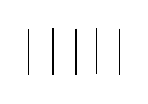
\begin{tikzpicture}[x=0.75pt,y=0.75pt,yscale=-1,xscale=1]
\draw    (100.31,116.42) -- (100.31,138.67) ;
\draw    (112.26,116) -- (112.26,138.25) ;
\draw    (123.33,116.14) -- (123.33,138.39) ;
\draw    (133.26,115.95) -- (133.26,138.19) ;
\draw    (144.33,116.09) -- (144.33,138.33) ;
\end{tikzpicture}
},
optionC={   
\tikzset{every picture/.style={line width=0.75pt,scale=\scalefactor}} 
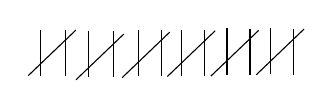
\begin{tikzpicture}[x=0.75pt,y=0.75pt,yscale=-1,xscale=1]
\draw    (276.33,114.14) -- (276.33,136.39) ;
\draw    (288.28,114) -- (288.28,136.25) ;
\draw    (299.36,114.28) -- (299.36,136.53) ;
\draw    (311.31,114.42) -- (311.31,136.67) ;
\draw    (293.28,114) -- (270.28,136) ;
\draw    (323.26,114) -- (323.26,136.25) ;
\draw    (334.33,114.14) -- (334.33,136.39) ;
\draw    (344.26,113.95) -- (344.26,136.19) ;
\draw    (355.33,114.09) -- (355.33,136.33) ;
\draw    (316.28,116) -- (293.28,138) ;
\draw    (338.48,115) -- (315.48,137) ;
\draw    (360.33,114.39) -- (337.33,136.39) ;
\draw    (366.06,113.2) -- (366.06,135.45) ;
\draw    (377.13,113.34) -- (377.13,135.59) ;
\draw    (387.06,113.15) -- (387.06,135.39) ;
\draw    (398.13,113.29) -- (398.13,135.53) ;
\draw    (381.28,114.2) -- (358.28,136.2) ;
\draw    (403.13,113.59) -- (380.13,135.59) ;
\end{tikzpicture}
},
optionD={
\tikzset{every picture/.style={line width=0.75pt,scale=\scalefactor}} 
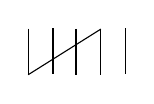
\begin{tikzpicture}[x=0.75pt,y=0.75pt,yscale=-1,xscale=1]
\draw    (98.33,161.14) -- (98.33,183.39) ;
\draw    (110.28,161) -- (110.28,183.25) ;
\draw    (121.36,161.28) -- (121.36,183.53) ;
\draw    (133.31,161.42) -- (133.31,183.67) ;
\draw    (133.31,161.42) -- (98.33,183.39) ;
\draw    (145.26,161) -- (145.26,183.25) ;
\end{tikzpicture}
},
questionTag={C6M17 – DT – Q1}, 
correctoption={D},
leftmini={0.5},
rightmini={0.4}
}

\begin{minipage}{\linewidth}
\hspace{1cm}
\centering
\tiny
\renewcommand{\arraystretch}{1.25}
\begin{tabular}{|M{1.2cm}|M{0.8cm}|M{0.8cm}|M{0.8cm}|M{0.8cm}|M{0.8cm}|}
\hline
Option & A (\ding{55}) & B (\ding{55}) & C (\ding{55}) & \cellcolor{cellgreen} D (\ding{51}) & E \\ 
\hline
6 A & \highno{0\%} & \highno{0\%} & \highno{7\%} & \highgreen{93\%} & \highno{0\%} \\ 
 \hline 
6 B & \highno{0\%} & \highno{0\%} & \highno{5\%} & \highgreen{89\%} & \highno{5\%} \\ \hline
\end{tabular}
\end{minipage}

\end{frame}
% \input{4. PPT/6. My Answer/Math/C6/117_C6M - Q46}


\begin{frame}[shrink=0.1,label=QPC6QC6M16 - DT - Q5]{Q13 [10. Mensuration]}
\vspace{-0.2cm}
\mcqtextbottomOneFour{
questionnumber={13}, 
questionTag={C6M16 - DT - Q5}, 
questiontext={Find the area of a square whose side is 65 m.},
optionA={ $65$ sq. cm},
optionB={$3925$ sq. m},
optionC={$6925$ sq. m},
optionD={$4225$ sq. m},
correctoption={D},
}

\begin{minipage}{\linewidth}
\hspace{1cm}
\centering
\tiny
\renewcommand{\arraystretch}{1.25}
\begin{tabular}{|M{1.2cm}|M{0.8cm}|M{0.8cm}|M{0.8cm}|M{0.8cm}|M{0.8cm}|}
\hline
Option & A (\ding{55}) & B (\ding{55}) & C (\ding{55}) & \cellcolor{cellgreen} D (\ding{51}) & E \\ 
\hline
6 A & \highno{7\%} & \highno{27\%} & \highno{7\%} & \highno{60\%} & \highno{0\%} \\ 
 \hline 
6 B & \highno{11\%} & \highno{16\%} & \highno{16\%} & \highno{58\%} & \highno{0\%} \\ \hline
\end{tabular}
\end{minipage}

\end{frame}
% \input{4. PPT/6. My Answer/Math/C6/117_C6M - Q13}


\begin{frame}[shrink=0.1,label=QPC6QC6M16 - DT - Q3]{Q16 [10. Mensuration]}
\vspace{-0.2cm}
\mcqimgleftFourOne{
questionnumber={16}, 
questionTag={C6M16 – DT – Q3},
questiontext={Which shape has the greater perimeter? },
imgtabletikz  = {\tikzset{every picture/.style={line width=0.75pt,scale=\scalefactor}} 
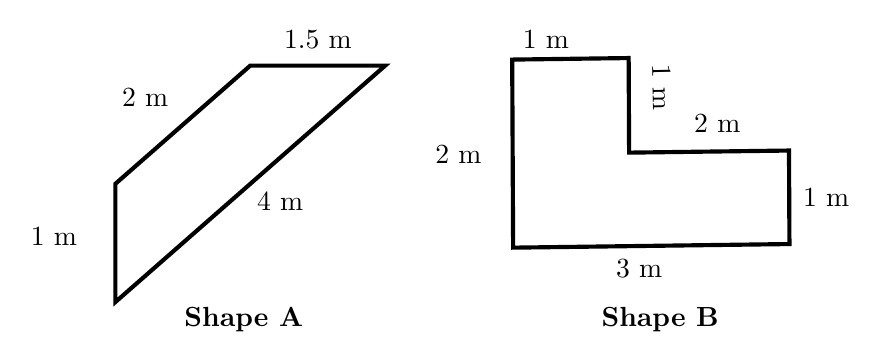
\begin{tikzpicture}[x=0.75pt,y=0.75pt,yscale=-1,xscale=1]

\draw  [line width=1.5]  (411.17,95.11) -- (467.28,94.37) -- (467.5,139.94) -- (544.53,138.93) -- (544.75,183.98) -- (411.62,185.72) -- cycle ;
\draw  [line width=1.5]  (285,98) -- (350,98) -- (220,211.92) -- (220,154.96) -- cycle ;
\draw (488.4,96.05) node [anchor=north west][inner sep=0.75pt]  [rotate=-88.86] [align=left] {1 m};
\draw (415,80) node [anchor=north west][inner sep=0.75pt]   [align=left] {1 m};
\draw (372.89,135.39) node [anchor=north west][inner sep=0.75pt]   [align=left] {2 m};
\draw (550.11,155.91) node [anchor=north west][inner sep=0.75pt]   [align=left] {1 m};
\draw (497.62,120.34) node [anchor=north west][inner sep=0.75pt]   [align=left] {2 m};
\draw (460,190) node [anchor=north west][inner sep=0.75pt]   [align=left] {3 m};
\draw (453,213) node [anchor=north west][inner sep=0.75pt]   [align=left] {\textbf{Shape B}};
\draw (178,175) node [anchor=north west][inner sep=0.75pt]   [align=left] {1 m};
\draw (222,108) node [anchor=north west][inner sep=0.75pt]   [align=left] {2 m};
\draw (300,80) node [anchor=north west][inner sep=0.75pt]   [align=left] {1.5 m};
\draw (287,157.96) node [anchor=north west][inner sep=0.75pt]   [align=left] {4 m};
\draw (252,213) node [anchor=north west][inner sep=0.75pt]   [align=left] {\textbf{Shape A}};
\end{tikzpicture}},
optionA={Shape A},
optionB={Shape B},
optionC={Both are equal},
optionD={Perimeter cannot be calculated},
correctoption={B},
leftmini={0.55},
rightmini={0.35},}

\begin{minipage}{\linewidth}
\hspace{1cm}
\centering
\tiny
\renewcommand{\arraystretch}{1.25}
\begin{tabular}{|M{1.2cm}|M{0.8cm}|M{0.8cm}|M{0.8cm}|M{0.8cm}|M{0.8cm}|}
\hline
Option & A (\ding{55}) & \cellcolor{cellgreen} B (\ding{51}) & C (\ding{55}) & D (\ding{55}) & E \\ 
\hline
6 A & \highno{33\%} & \highno{67\%} & \highno{0\%} & \highno{0\%} & \highno{0\%} \\ 
 \hline 
6 B & \highno{5\%} & \highgreen{95\%} & \highno{0\%} & \highno{0\%} & \highno{0\%} \\ \hline
\end{tabular}
\end{minipage}

\end{frame}
% \input{4. PPT/6. My Answer/Math/C6/117_C6M - Q16}


\begin{frame}[shrink=0.1,label=QPC6QC6M16 - DT - Q6]{Q21 [10. Mensuration]}
\vspace{-0.2cm}
\mcqimgleftFourOne{
questionnumber={21}, 
questionTag={C6M16 - DT - Q6},
questiontext={Find the area of the given shape.},
imgtabletikz  = {

\tikzset{every picture/.style={line width=0.75pt,scale=\scalefactor}} 
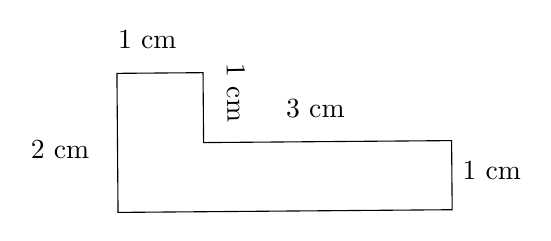
\begin{tikzpicture}[x=0.75pt,y=0.75pt,yscale=-1,xscale=1]
\draw   (119.74,86.74) -- (161.22,86.41) -- (161.49,120.1) -- (280.98,119.14) -- (281.25,152.44) -- (120.27,153.74) -- cycle ;
\draw (200,98) node [anchor=north west][inner sep=0.75pt]   [align=left] {3 cm};
\draw (285,128) node [anchor=north west][inner sep=0.75pt]   [align=left] {1 cm};
\draw (77,118) node [anchor=north west][inner sep=0.75pt]   [align=left] {2 cm};
\draw (119,65) node [anchor=north west][inner sep=0.75pt]   [align=left] {1 cm};
\draw (182.38,80.74) node [anchor=north west][inner sep=0.75pt]  [rotate=-88.86] [align=left] {1 cm};
\end{tikzpicture}},
optionA={17 sq. cm},
optionB={8 sq. cm},
optionC={5 sq. cm},
optionD={4 sq. m},
correctoption={C},
leftmini={0.5},
rightmini={0.4},
}

\begin{minipage}{\linewidth}
\hspace{1cm}
\centering
\tiny
\renewcommand{\arraystretch}{1.25}
\begin{tabular}{|M{1.2cm}|M{0.8cm}|M{0.8cm}|M{0.8cm}|M{0.8cm}|M{0.8cm}|}
\hline
Option & A (\ding{55}) & B (\ding{55}) & \cellcolor{cellgreen} C (\ding{51}) & D (\ding{55}) & E \\ 
\hline
6 A & \highno{0\%} & \highno{87\%} & \highred{7\%} & \highno{0\%} & \highno{7\%} \\ 
 \hline 
6 B & \highno{11\%} & \highno{63\%} & \highred{26\%} & \highno{0\%} & \highno{0\%} \\ \hline
\end{tabular}
\end{minipage}

\end{frame}
\begin{frame}{Q21 - My Answer Responses}
    \vspace{-0.6cm}
    \begin{multicols}{3}

    % Image: Q21_D117140_Math.png - Scaled height: 3.36mm
    \begin{minipage}{\linewidth}
    \RaggedRight\textbf{\tiny \highred{Sabarish B [B]}} \\ 
    \vspace{4.00pt}\fcolorbox{blue}{white}{\includegraphics[width=3cm]{Q21_D117140_Math.png}}
    \end{minipage}
    \vspace{10pt}

    % Image: Q21_D117146_Math.png - Scaled height: 3.84mm
    \begin{minipage}{\linewidth}
    \RaggedRight\textbf{\tiny \highred{Aashinisri G [B]}} \\ 
    \vspace{4.00pt}\fcolorbox{blue}{white}{\includegraphics[width=3cm]{Q21_D117146_Math.png}}
    \end{minipage}
    \vspace{10pt}

    % Image: Q21_D117151_Math.png - Scaled height: 5.40mm
    \begin{minipage}{\linewidth}
    \RaggedRight\textbf{\tiny \highred{Karnika R [B]}} \\ 
    \vspace{4.00pt}\fcolorbox{blue}{white}{\includegraphics[width=3cm]{Q21_D117151_Math.png}}
    \end{minipage}
    \vspace{10pt}

    % Image: Q21_D117153_Math.png - Scaled height: 7.20mm
    \begin{minipage}{\linewidth}
    \RaggedRight\textbf{\tiny \highred{Priyadharshini S A [B]}} \\ 
    \vspace{4.00pt}\fcolorbox{blue}{white}{\includegraphics[width=3cm]{Q21_D117153_Math.png}}
    \end{minipage}
    \vspace{10pt}

    % Image: Q21_D117157_Math.png - Scaled height: 4.54mm
    \begin{minipage}{\linewidth}
    \RaggedRight\textbf{\tiny \highred{Aswin P [B]}} \\ 
    \vspace{4.00pt}\fcolorbox{blue}{white}{\includegraphics[width=3cm]{Q21_D117157_Math.png}}
    \end{minipage}
    \vspace{10pt}

    % Image: Q21_D117161_Math.png - Scaled height: 5.64mm
    \begin{minipage}{\linewidth}
    \RaggedRight\textbf{\tiny \highred{Kiruthik D [B]}} \\ 
    \vspace{4.00pt}\fcolorbox{blue}{white}{\includegraphics[width=3cm]{Q21_D117161_Math.png}}
    \end{minipage}
    \vspace{10pt}

    % Image: Q21_D117163_Math.png - Scaled height: 7.33mm
    \begin{minipage}{\linewidth}
    \RaggedRight\textbf{\tiny \highred{Manjunath A [B]}} \\ 
    \vspace{4.00pt}\fcolorbox{blue}{white}{\includegraphics[width=3cm]{Q21_D117163_Math.png}}
    \end{minipage}
    \vspace{10pt}

    % Image: Q21_D117167_Math.png - Scaled height: 3.90mm
    \begin{minipage}{\linewidth}
    \RaggedRight\textbf{\tiny \highgreen{Sriram Karthikeyan V [C]}} \\ 
    \vspace{4.00pt}\fcolorbox{blue}{white}{\includegraphics[width=3cm]{Q21_D117167_Math.png}}
    \end{minipage}
    \vspace{10pt}

    % Image: Q21_D117172_Math.png - Scaled height: 4.59mm
    \begin{minipage}{\linewidth}
    \RaggedRight\textbf{\tiny \highred{Raksha Nivasini K S [B]}} \\ 
    \vspace{4.00pt}\fcolorbox{blue}{white}{\includegraphics[width=3cm]{Q21_D117172_Math.png}}
    \end{minipage}
    \vspace{10pt}

    \end{multicols}
\end{frame}




\begin{frame}[shrink=0.1,label=QPC6QC6M16 - DT - Q4]{Q40 [10. Mensuration]}
\vspace{-0.2cm}
\mcqimgleftFourOne{
questionnumber={40}, 
questionTag={C6M16 - DT - Q4}, 
questiontext={Find the area of the given rectangular notebook.},
imgtabletikz  = {
\tikzset{every picture/.style={line width=0.75pt,scale=\scalefactor}} 
\begin{tikzpicture}[x=0.75pt,y=0.75pt,yscale=-1,xscale=1]
\draw (244.25,113.49) node  {\adjustbox{scale=\scalefactor}{\includegraphics[width=81.38pt,height=95.24pt]{C6M16 - DT - Q4.png}}};
\draw [line width=1.5]    (303.41,66.12) -- (302.75,165.15) ;
\draw [shift={(302.73,169.15)}, rotate = 270.38] [fill={rgb, 255:red, 0; green, 0; blue, 0 }  ][line width=0.08]  [draw opacity=0] (11.61,-5.58) -- (0,0) -- (11.61,5.58) -- cycle    ;
\draw [shift={(303.43,62.12)}, rotate = 90.38] [fill={rgb, 255:red, 0; green, 0; blue, 0 }  ][line width=0.08]  [draw opacity=0] (11.61,-5.58) -- (0,0) -- (11.61,5.58) -- cycle    ;
\draw [line width=1.5]    (288.16,183.81) -- (208.8,183.17) ;
\draw [shift={(204.8,183.14)}, rotate = 0.46] [fill={rgb, 255:red, 0; green, 0; blue, 0 }  ][line width=0.08]  [draw opacity=0] (11.61,-5.58) -- (0,0) -- (11.61,5.58) -- cycle    ;
\draw [shift={(292.16,183.84)}, rotate = 180.46] [fill={rgb, 255:red, 0; green, 0; blue, 0 }  ][line width=0.08]  [draw opacity=0] (11.61,-5.58) -- (0,0) -- (11.61,5.58) -- cycle    ;
\draw (307.65,109.71) node [anchor=north west][inner sep=0.75pt]   [align=left] {45 cm};
\draw (224.51,190.15) node [anchor=north west][inner sep=0.75pt]   [align=left] {31 cm};
\end{tikzpicture} },
optionA={ $1395$ cm},
optionB={$2025$ cm},
optionC={$1395$ sq. cm},
optionD={$2025$ sq. cm},
correctoption={C},
leftmini={0.5},
rightmini={0.4},
}

\begin{minipage}{\linewidth}
\hspace{1cm}
\centering
\tiny
\renewcommand{\arraystretch}{1.25}
\begin{tabular}{|M{1.2cm}|M{0.8cm}|M{0.8cm}|M{0.8cm}|M{0.8cm}|M{0.8cm}|}
\hline
Option & A (\ding{55}) & B (\ding{55}) & \cellcolor{cellgreen} C (\ding{51}) & D (\ding{55}) & E \\ 
\hline
6 A & \highno{27\%} & \highno{0\%} & \highno{67\%} & \highno{7\%} & \highno{0\%} \\ 
 \hline 
6 B & \highno{21\%} & \highno{11\%} & \highno{63\%} & \highno{0\%} & \highno{5\%} \\ \hline
\end{tabular}
\end{minipage}

\end{frame}
% \input{4. PPT/6. My Answer/Math/C6/117_C6M - Q40}


\begin{frame}[shrink=0.1,label=QPC6QC6M16 - DT - Q9]{Q57 [10. Mensuration]}
\vspace{-0.2cm}
\mcqimgleftFourOne{
questionnumber={57}, 
questionTag={C6M16 - DT - Q9},
questiontext={Ramu walks around the lake in the evening. The path he walked is to be considered as the \rule{80pt}{0.5pt}},
imgtabletikz = { \adjustbox{scale=\scalefactor}{\includegraphics[width=3cm, height=3.5cm]{C6M16 - DT - Q9.png}}},
optionA={Area},
optionB={Perimeter},
optionC={Volume},
optionD={Both a and b},
correctoption={B},
leftmini={0.4},
rightmini={0.5},
}

\begin{minipage}{\linewidth}
\hspace{1cm}
\centering
\tiny
\renewcommand{\arraystretch}{1.25}
\begin{tabular}{|M{1.2cm}|M{0.8cm}|M{0.8cm}|M{0.8cm}|M{0.8cm}|M{0.8cm}|}
\hline
Option & A (\ding{55}) & \cellcolor{cellgreen} B (\ding{51}) & C (\ding{55}) & D (\ding{55}) & E \\ 
\hline
6 A & \highno{27\%} & \highno{67\%} & \highno{0\%} & \highno{7\%} & \highno{0\%} \\ 
 \hline 
6 B & \highno{21\%} & \highno{58\%} & \highno{0\%} & \highno{21\%} & \highno{0\%} \\ \hline
\end{tabular}
\end{minipage}

\end{frame}
% \input{4. PPT/6. My Answer/Math/C6/117_C6M - Q57}


\begin{frame}[shrink=0.1,label=QPC6QC6M16 - CT - Q1]{Q60 [10. Mensuration]}
\vspace{-0.2cm}
\mcqtextbottomOneFour{
questionnumber={60 - Critical Thinking},
questionTag = {C6M16 - CT - Q1},
questiontext = {The length of one side of the square-shaped farm is 9 m. Rithu cycles around the farm twice a day, once in the morning and once in the evening. Find the unit digit of the distance covered by her in a day.},
optionA={6},
optionB={8},
optionC={2},
optionD={9},
correctoption = {C},
}

\begin{minipage}{\linewidth}
\hspace{1cm}
\centering
\tiny
\renewcommand{\arraystretch}{1.25}
\begin{tabular}{|M{1.2cm}|M{0.8cm}|M{0.8cm}|M{0.8cm}|M{0.8cm}|M{0.8cm}|}
\hline
Option & A (\ding{55}) & B (\ding{55}) & \cellcolor{cellgreen} C (\ding{51}) & D (\ding{55}) & E \\ 
\hline
6 A & \highno{13\%} & \highno{20\%} & \highred{27\%} & \highno{40\%} & \highno{0\%} \\ 
 \hline 
6 B & \highno{5\%} & \highno{37\%} & \highred{5\%} & \highno{47\%} & \highno{5\%} \\ \hline
\end{tabular}
\end{minipage}

\end{frame}
% \input{4. PPT/6. My Answer/Math/C6/117_C6M - Q60 - Critical Thinking}


\begin{frame}[shrink=0.1,label=QPC6QC6M09 - DT - Q2]{Q17 [11. Algebra]}
\vspace{-0.2cm}
\mcqimgleftFourOne{
questionnumber={17}, 
questionTag={C6M09 - DT - Q2}, 
questiontext={How many line segments are required to make $n$ number of the given shape?},
imgtabletikz  = {\tikzset{every picture/.style={line width=0.75pt,scale=\scalefactor}} 
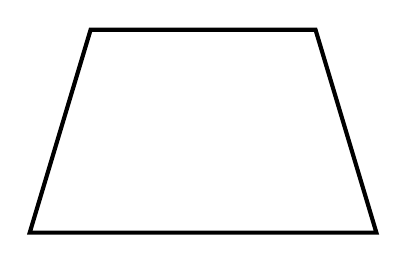
\begin{tikzpicture}[x=0.75pt,y=0.75pt,yscale=-1,xscale=1]
\draw  [line width=1.5]  (149,189.73) -- (178.32,92) -- (286.68,92) -- (316,189.73) -- cycle ;
\end{tikzpicture}},
optionA={$n$},
optionB={4},
optionC={4$n$},
optionD={$ n \times n $},
correctoption={C},
leftmini={0.4},
rightmini={0.5},
}

\begin{minipage}{\linewidth}
\hspace{1cm}
\centering
\tiny
\renewcommand{\arraystretch}{1.25}
\begin{tabular}{|M{1.2cm}|M{0.8cm}|M{0.8cm}|M{0.8cm}|M{0.8cm}|M{0.8cm}|}
\hline
Option & A (\ding{55}) & B (\ding{55}) & \cellcolor{cellgreen} C (\ding{51}) & D (\ding{55}) & E \\ 
\hline
6 A & \highno{0\%} & \highno{33\%} & \highno{53\%} & \highno{13\%} & \highno{0\%} \\ 
 \hline 
6 B & \highno{5\%} & \highno{16\%} & \highno{63\%} & \highno{16\%} & \highno{0\%} \\ \hline
\end{tabular}
\end{minipage}

\end{frame}
% \input{4. PPT/6. My Answer/Math/C6/117_C6M - Q17}


\begin{frame}[shrink=0.1,label=QPC6QC6M09 - DT - Q1]{Q18 [11. Algebra]}
\vspace{-0.2cm}
\mcqtextbottomOneFour{
questionnumber={18}, 
questionTag={C6M09 - DT - Q1}, 
questiontext={How many variables are present in the expression $5x + 4y - 3z+2x-y$?},
optionA={ 5},
optionB={ 3},
optionC={ 2},
optionD={ 4},
correctoption={B},
}

\begin{minipage}{\linewidth}
\hspace{1cm}
\centering
\tiny
\renewcommand{\arraystretch}{1.25}
\begin{tabular}{|M{1.2cm}|M{0.8cm}|M{0.8cm}|M{0.8cm}|M{0.8cm}|M{0.8cm}|}
\hline
Option & A (\ding{55}) & \cellcolor{cellgreen} B (\ding{51}) & C (\ding{55}) & D (\ding{55}) & E \\ 
\hline
6 A & \highno{40\%} & \highred{0\%} & \highno{0\%} & \highno{53\%} & \highno{7\%} \\ 
 \hline 
6 B & \highno{32\%} & \highred{11\%} & \highno{26\%} & \highno{32\%} & \highno{0\%} \\ \hline
\end{tabular}
\end{minipage}

\end{frame}
% \input{4. PPT/6. My Answer/Math/C6/117_C6M - Q18}


\begin{frame}[shrink=0.1,label=QPC6QC6M09 - DT - Q3]{Q51 [11. Algebra]}
\vspace{-0.2cm}
\mcqimgleftFourOne{
questionnumber={51}, 
questionTag={C6M09 - DT - Q3},
questiontext={Match the following.},
imgtabletikz  = { \begin{table}[H]
\centering
\renewcommand{\arraystretch}{1.25}
\begin{tabular}{|p{0.4cm}|p{4cm}|p{0.2cm}|p{0.4cm}|p{1cm}|}
\cline{1-5} 
\multicolumn{2}{|c|}{\textbf{Statement }} & 
\multirow{5}{*}{} &   
\multicolumn{2}{c|}{\textbf{Expression}} \\
\cline{1-2}\cline{4-5} i.  & 10 times of $y$ is added to 5
&   & a. & $-$10$y$ \\
\cline{1-2}\cline{4-5} ii. & 10 less than a number is 5
&   & b. &  10$y$$+$5\\
\cline{1-2}\cline{4-5} iii.  & 10 is multiplied by $-$$y$
&   & c. & $y$$-$10 = 5 \\
\hline
\end{tabular}
\end{table}},
optionA={i - c, ii - b, iii - a},
optionB={i - a, ii - b, iii - c},
optionC={i - a, ii - c, iii - b},
optionD={i - b, ii - c, iii - a},
correctoption={D},
leftmini={0.6},
rightmini={0.3},
}

\begin{minipage}{\linewidth}
\hspace{1cm}
\centering
\tiny
\renewcommand{\arraystretch}{1.25}
\begin{tabular}{|M{1.2cm}|M{0.8cm}|M{0.8cm}|M{0.8cm}|M{0.8cm}|M{0.8cm}|}
\hline
Option & A (\ding{55}) & B (\ding{55}) & C (\ding{55}) & \cellcolor{cellgreen} D (\ding{51}) & E \\ 
\hline
6 A & \highno{0\%} & \highno{13\%} & \highno{7\%} & \highgreen{80\%} & \highno{0\%} \\ 
 \hline 
6 B & \highno{11\%} & \highno{5\%} & \highno{5\%} & \highgreen{79\%} & \highno{0\%} \\ \hline
\end{tabular}
\end{minipage}

\end{frame}
% \input{4. PPT/6. My Answer/Math/C6/117_C6M - Q51}


\begin{frame}[shrink=0.1,label=QPC6QC6M10 - DT - Q6]{Q15 [12. Ratio and Proportion]}
\vspace{-0.2cm}
\mcqtextbottomOneFour{
questionnumber={15}, 
questionTag={C6M10 - DT - Q6}, 
questiontext={If one milkshake costs Rs. 35, how many milkshakes can you buy for Rs. 140?},
optionA={ 4},
optionB={ 8 },
optionC={5},
optionD={ 10},
correctoption={A},
}

\begin{minipage}{\linewidth}
\hspace{1cm}
\centering
\tiny
\renewcommand{\arraystretch}{1.25}
\begin{tabular}{|M{1.2cm}|M{0.8cm}|M{0.8cm}|M{0.8cm}|M{0.8cm}|M{0.8cm}|}
\hline
Option & \cellcolor{cellgreen} A (\ding{51}) & B (\ding{55}) & C (\ding{55}) & D (\ding{55}) & E \\ 
\hline
6 A & \highgreen{93\%} & \highno{0\%} & \highno{0\%} & \highno{0\%} & \highno{7\%} \\ 
 \hline 
6 B & \highno{74\%} & \highno{5\%} & \highno{11\%} & \highno{11\%} & \highno{0\%} \\ \hline
\end{tabular}
\end{minipage}

\end{frame}
% \input{4. PPT/6. My Answer/Math/C6/117_C6M - Q15}


\begin{frame}[shrink=0.1,label=QPC6QC6M10 - DT - Q5]{Q19 [12. Ratio and Proportion]}
\vspace{-0.2cm}
\mcqtextbottomOneFour{
questionnumber={19}, 
questionTag={C6M10 - DT - Q5}, 
questiontext={Find the value of $x$ in the following proportion.\quad 10 : 8 : : $x$ : 24},
optionA={ 30},
optionB={ 35 },
optionC={100},
optionD={ 50},
correctoption={A},
}

\begin{minipage}{\linewidth}
\hspace{1cm}
\centering
\tiny
\renewcommand{\arraystretch}{1.25}
\begin{tabular}{|M{1.2cm}|M{0.8cm}|M{0.8cm}|M{0.8cm}|M{0.8cm}|M{0.8cm}|}
\hline
Option & \cellcolor{cellgreen} A (\ding{51}) & B (\ding{55}) & C (\ding{55}) & D (\ding{55}) & E \\ 
\hline
6 A & \highno{60\%} & \highno{13\%} & \highno{27\%} & \highno{0\%} & \highno{0\%} \\ 
 \hline 
6 B & \highno{53\%} & \highno{32\%} & \highno{11\%} & \highno{5\%} & \highno{0\%} \\ \hline
\end{tabular}
\end{minipage}

\end{frame}
% \input{4. PPT/6. My Answer/Math/C6/117_C6M - Q19}


\begin{frame}[shrink=0.1,label=QPC6QC6M10 - DT - Q1]{Q43 [12. Ratio and Proportion]}
\vspace{-0.2cm}
\mcqtextbottomOneFour{
questionnumber={43}, 
questionTag={C6M10 - DT - Q1}, 
questiontext={Write {{$\dfrac{1}{10}$}} in the form of ratio. },
optionA={ 1 : 1},
optionB={10 : 1},
optionC={1 : 10},
optionD={1 : 1, 10 : 10},
correctoption={C},
}

\begin{minipage}{\linewidth}
\hspace{1cm}
\centering
\tiny
\renewcommand{\arraystretch}{1.25}
\begin{tabular}{|M{1.2cm}|M{0.8cm}|M{0.8cm}|M{0.8cm}|M{0.8cm}|M{0.8cm}|}
\hline
Option & A (\ding{55}) & B (\ding{55}) & \cellcolor{cellgreen} C (\ding{51}) & D (\ding{55}) & E \\ 
\hline
6 A & \highno{13\%} & \highno{20\%} & \highno{67\%} & \highno{0\%} & \highno{0\%} \\ 
 \hline 
6 B & \highno{5\%} & \highno{11\%} & \highgreen{79\%} & \highno{5\%} & \highno{0\%} \\ \hline
\end{tabular}
\end{minipage}

\end{frame}
% \input{4. PPT/6. My Answer/Math/C6/117_C6M - Q43}


\begin{frame}[shrink=0.1,label=QPC6QC6M10 - DT - Q7]{Q44 [12. Ratio and Proportion]}
\vspace{-0.2cm}
\mcqtextbottomOneFour{
questionnumber={44}, 
questionTag={C6M10 - DT - Q7}, 
questiontext={Anu and Abi ate chocolates in the ratio 4 : 9. If Abi ate 36 chocolates, find the number of chocolates eaten by Anu.},
optionA={ 16 chocolates},
optionB={ 81 chocolates },
optionC={ 72 chocolates},
optionD={ 56 chocolates},
correctoption={A},
}

\begin{minipage}{\linewidth}
\hspace{1cm}
\centering
\tiny
\renewcommand{\arraystretch}{1.25}
\begin{tabular}{|M{1.2cm}|M{0.8cm}|M{0.8cm}|M{0.8cm}|M{0.8cm}|M{0.8cm}|}
\hline
Option & \cellcolor{cellgreen} A (\ding{51}) & B (\ding{55}) & C (\ding{55}) & D (\ding{55}) & E \\ 
\hline
6 A & \highno{47\%} & \highno{20\%} & \highno{7\%} & \highno{20\%} & \highno{7\%} \\ 
 \hline 
6 B & \highno{42\%} & \highno{11\%} & \highno{21\%} & \highno{16\%} & \highno{11\%} \\ \hline
\end{tabular}
\end{minipage}

\end{frame}
% \input{4. PPT/6. My Answer/Math/C6/117_C6M - Q44}


\begin{frame}[shrink=0.1,label=QPC6QC6M10 - DT - Q9]{Q55 [12. Ratio and Proportion]}
\vspace{-0.2cm}
\mcqtextbottomOneFour{
questionnumber={55}, 
questionTag={C6M10 - DT - Q9},
questiontext={If one quantity in the ratio is 8 g, the unit of the other quantity should be in \rule{80pt}{0.5pt}, to compare them. },
optionA={gram},
optionB={kilogram},
optionC={liter},
optionD={Either a and b},
correctoption={A},
}

\begin{minipage}{\linewidth}
\hspace{1cm}
\centering
\tiny
\renewcommand{\arraystretch}{1.25}
\begin{tabular}{|M{1.2cm}|M{0.8cm}|M{0.8cm}|M{0.8cm}|M{0.8cm}|M{0.8cm}|}
\hline
Option & \cellcolor{cellgreen} A (\ding{51}) & B (\ding{55}) & C (\ding{55}) & D (\ding{55}) & E \\ 
\hline
6 A & \highno{40\%} & \highno{27\%} & \highno{7\%} & \highno{20\%} & \highno{7\%} \\ 
 \hline 
6 B & \highno{58\%} & \highno{26\%} & \highno{0\%} & \highno{11\%} & \highno{5\%} \\ \hline
\end{tabular}
\end{minipage}

\end{frame}
% \input{4. PPT/6. My Answer/Math/C6/117_C6M - Q55}

%

    